%%% Master-File f"ur Diplomarbeit
%%% Time-stamp: <1999-03-05 11:51:53 ralf>
%
%\documentclass[12pt,german,a4paper,draft]{book}
% draft ausschalten, um Bilder anzuzeigen
\documentclass[12pt,german,a4paper]{book}
% brauche ich immer
\usepackage{babel,latexsym,amsmath,amssymb}
% zum Einbinden von .eps files
\usepackage[dvips]{graphicx}
% sch?ne headings
\usepackage{fancyhdr}
% Rotieren von Objekten
\usepackage{rotating,lscape,rotfloat}
% narrow floating figures and tables
\usepackage{floatflt}
% erm?glicht eqnarrays mit allen tabular Befehlen
\usepackage{eqnarray}
% Mehr Kontrolle ?ber floats
\usepackage{afterpage,float}

% floating equation, rotierbar
\newfloat{floateq}{tpbh}{feq}[chapter]
\floatname{floateq}{Gleichung}
% \setcounter{floateq}{\value{equation}}
% macht Numerierung Einheitlich zu equations
\newenvironment{floateqnum}{\setcounter{floateq}{\value{equation}}\begin{floateq}}{\end{floateq}}
\newenvironment{sidewaysfloateqnum}{\setcounter{floateq}{\value{equation}}\begin{sidewaysfloateq}}{\end{sidewaysfloateq}}

% mathe.tex
% Time-stamp: <1999-09-23 19:34:49 ralf>
%
% Mathematisches allerlei
%
\DeclareMathAlphabet{\mathsfbf}{T1}{cmss}{bx}{n}
\DeclareMathAlphabet{\mathcalbf}{U}{eus}{b}{n}
%
% mathematische Objekte
%
\newcommand{\Matrix}[1]{\ensuremath{#1}}
% Operator (ohne Hut)
\newcommand{\op}[1]{\ensuremath{\protect #1}}
\newcommand{\vecop}[1]{\ensuremath{\mathbf{\protect #1}}}
\newcommand{\grvecop}[1]{\mbox{\mathversion{bold}$\protect #1$}}
%
\newcommand{\menge}[1]{\ensuremath{\mathcal{#1}}}
\newcommand{\raum}[1]{\ensuremath{\mathsf{#1}}}
\renewcommand{\vec}[1]{\ensuremath{\mathbf{#1}}}
\newcommand{\grvec}[1]{\mbox{\mathversion{bold}$#1$}}
% Einheitsvectoren
\newcommand{\ex}{\ensuremath{\vec{\protect\hat e}_{x}}}
\newcommand{\ey}{\ensuremath{\vec{\protect\hat e}_{y}}}
\newcommand{\ez}{\ensuremath{\vec{\protect\hat e}_{z}}}
%
% Operationen/Operatoren
%
% hermitesch konjugiert, transponiert, komplex konjugiert
\newcommand{\hc}[1]{\ensuremath{#1^{\dagger}}}
\newcommand{\transp}[1]{\ensuremath{#1^{\mathsf{T}}}}
\newcommand{\cc}[1]{\ensuremath{#1^{\ast}}}
% Skalarprodukt <#1, #2> und vec.vec 
\newcommand{\scp}[2]{\ensuremath{\left\langle {#1}, {#2} \right\rangle}}
\newcommand{\sprod}[2]{\ensuremath{\vec{#1} \cdot \vec{#2} }}
% Kommutator [#1, #2]
\newcommand{\kom}[2]{\ensuremath{\left [\, {#1}, {#2} \, \right] }}
% Antikommutator {#1, #2}
\newcommand{\akom}[2]{\ensuremath{\left \{\, {#1}, {#2} \, \right \}}}
% Poissonklammern
\newcommand{\poisson}[2]{\akom{#1}{#2}}
% Ableitungen etc.
\newcommand{\dx}[1]{d#1\,}
\newcommand{\vdx}[1]{d^{3}\!\!\: #1\,}
\newcommand{\ddx}[1]{\frac{d}{d#1}}
\newcommand{\pdx}[1]{\frac{\partial}{\partial#1}}
% Benannte mathem. Objekte
\newcommand{\kronecker}[2]{\ensuremath{\delta_{#1\,#2}}}
\newcommand{\Rn}[1]{\ensuremath{\real^{#1}}}
% Konstanten
\newcommand{\eins}{\ensuremath{\mathsf{1}}}
\newcommand{\halb}{\ensuremath{\frac{1}{2}}}
\newcommand{\veps}{\varepsilon}
\newcommand{\vphi}{\varphi}
\newcommand{\element}{\,\in\,}
% bra und ket etc...
\newcommand{\bra}[1]{\ensuremath{\langle {#1}|}}
\newcommand{\ket}[1]{\ensuremath{| {#1} \rangle}}
\newcommand{\braket}[2]{\ensuremath{\langle {#1} | {#2} \rangle}}
\newcommand{\matrixel}[3]{\ensuremath{\langle {#1} | {#2} | {#3} \rangle}}
\newcommand{\expect}[1]{\ensuremath{\langle {#1} \rangle}}
% f�r gro�e Eintr�ge
\newcommand{\Bra}[1]{\ensuremath{\left\langle {#1} \right|}}
\newcommand{\Ket}[1]{\ensuremath{\left| {#1} \right\rangle}}
\newcommand{\BraKet}[2]{\ensuremath{\left\langle {#1} | {#2} \right\rangle}}
\newcommand{\Matrixel}[3]{\ensuremath{\left\langle {#1}%
\left| {#2} \right| {#3} \right\rangle}}
\newcommand{\Expect}[1]{\ensuremath{\left\langle {#1} \right\rangle}}

%%%%%%%%%%%%%%%%%%%%%%%%%%%%%%%%%%%%%%%%%%%%%%%%%%%%%%
% von Roland 

%  %  \newcommand {\arc}{\mbox{$\rm <\hspace{-0.6em}
%  %               \raise0.3ex\hbox{$\scriptscriptstyle )$}$}}

\newcommand{\vektor}[1]{\ensuremath{\underline{\bf #1}}}
%\newcommand {\PSI}{\ensuremath{\mathbf{\underline{\psi}}}}
%\newcommand {\Matrix}[1]{\ensuremath{\underline{\underline{\bf #1}}}}
%\newcommand {\ableit}{\ensuremath{\frac{1}{i}\partial_z}}
\newcommand{\kdotp}{\ensuremath{\bf k \cdot p}}
\newcommand{\kreuz}{\ensuremath{\times}}
\newcommand{\eps}{\ensuremath{\varepsilon}}
% waum gibt es hier fehler???
%  \newcommand{\epsfett}[0][]{\mbox{\mathversion{bold}$#1 \varepsilon$}}
%  \newcommand{\pifett}[0][]{\mbox{\mathversion{bold}$#1 \pi$}}
%  \newcommand{\sigmafett}[0][]{\mbox{\mathversion{bold}$#1 \sigma$}}
%  \newcommand{\rhofett}[0][]{\mbox{\mathversion{bold}$#1 \sigmapi$}}
\newcommand{\BETA}[2]{\ensuremath{\displaystyle \frac{\hbar^2 #1}{2 m #2}}}
\newcommand{\spur}{{\mbox{tr}\hspace{0.3ex}}}
\newcommand{\kk}{\ensuremath{{\bf k}}}
\newcommand{\pp}{\ensuremath{{\bf p}}}
\newcommand{\rr}{\ensuremath{{\bf r}}}
\newcommand{\Qq}{\ensuremath{{\bf Q}}}
\newcommand{\dd}{{\rm d}}
\newcommand{\Ee}{\ensuremath{\mathcal E}}
\newcommand{\EE}{\mbox{\mathversion{bold}$\mathcal E$}}
\newcommand{\EEk}{\mbox{\small\mathversion{bold}$\cal E$}}
\newcommand{\ee}{{\rm e}}

\newcommand{\natur}{\mbox{\rm I\hspace{-0.12em}N}}
\newcommand{\real}{\mbox{\rm I\hspace{-0.12em}R}}
\newcommand{\komplex}{\mbox{\rm%
\hspace{0.7ex}\rule[0.15ex]{0.10ex}{1.35ex}\hspace{-0.7ex}C}}

\newcommand{\rational}{\mbox{\rm%
\hspace{0.7ex}\rule[0.15ex]{0.10ex}{1.35ex}\hspace{-0.7ex}Q}}

\newcommand{\indizes}[1]{{\mbox{\scriptsize #1}}}

\newcommand{\Ds}{\displaystyle}
\newcommand{\Ts}{\textstyle}
\newcommand{\Ss}{\scriptstyle}
\newcommand{\SSs}{\scriptscriptstyle}

% \newcommand {\bkopf}[1]{\refstepcounter{figure}\label{#1}Fig.\ \ref{#1}:}

% \newcounter{eintrag}
% \newenvironment{liste}[1]{\begin{list}{#1}{\usecounter{eintrag}%
%    \labelwidth1em \leftmargin1.5em \labelsep0.5em \itemsep0ex
%    \rightmargin0pt \topsep-\parskip \addtolength{\topsep}{1ex}%
%    \partopsep1ex \parsep0.6ex}}{\end{list}}

% \newenvironment{einrueck}[1]{\begin{list}{}{%
%    \settowidth{\labelwidth}{#1}%              Argument=Textstring
%    \setlength{\leftmargin}{\labelwidth}%
%    \addtolength{\leftmargin}{\labelsep}%
%    \parsep0.5ex plus0.2ex minus 0.2ex
%    \itemsep0.3ex
%    \renewcommand{\makelabel}[1]{##1\hfill}}}{\end{list}}

% \newenvironment{Einrueck}[1]{\begin{list}{}{%
%    \labelwidth#1%                              Argument=Massangabe
%    \labelsep1em
%    \setlength{\leftmargin}{\labelwidth}%
%    \addtolength{\leftmargin}{\labelsep}%
%    \parsep0.5ex plus0.2ex minus 0.2ex
%    \itemsep0.3ex
%    \renewcommand{\makelabel}[1]{##1\hfill}}}{\end{list}}

%%%%%%%%%%%%%%%%%%%%%%%%%%%%%%%%%%%%%%%%%%%%%%%%%%%%%%%%%%%%%%%%%

% \def\lesssim{\raisebox{0pt}[1pt][0pt]{$
%    \begin{array}{c}{<}\\[-1.6ex]{\sim}\end{array}$}}
% \def\gtrsim{\raisebox{0pt}[1pt][0pt]{$
%    \begin{array}{c}{>}\\[-1.6ex]{\sim}\end{array}$}}

% % \newcolumntype {s}[1]{@{\hspace{#1}}}
% \def\openone{\leavevmode\hbox{\small1\kern-0.8ex\normalsize1}}

% \endinput

%%% Local Variables: 
%%% mode: latex
%%% TeX-master: t
%%% End: 

%%% Definitionen f�r Diplomarbeit
%%% Time-stamp: <1999-06-01 17:11:35 ralf>

% primed 
\newcommand{\pri}[1]{\ensuremath{#1^{\prime}}}
% k in aBZ
\newcommand{\ak}{\grvec{\kappa}}
\newcommand{\akb}{\ensuremath{\kappa}}
% k in nBZ
\newcommand{\nk}{\vec{k}}
\newcommand{\nkb}{\ensuremath{k}}
% Set an k-punkten
%\newcommand{\set}{\vec{K}}
\newcommand{\set}{\ensuremath{\mathcalbf{K}}}
% reziproke Gittervektoren
\newcommand{\aG}{\ensuremath{\mathcalbf{G}_{\mathnormal{m}}}}
\newcommand{\paG}{\ensuremath{\mathcalbf{G}_{\mathnormal{\pri{m}}}}}
\newcommand{\nG}{\ensuremath{\vec{G}_{\mathnormal{m}}}}
\newcommand{\pnG}{\ensuremath{\vec{G}_{\mathnormal{\pri{m}}}}}
% Basisfunktionen
\newcommand{\altebasis}{\ensuremath{\phi_{n \ak}}}
\newcommand{\paltebasis}{\ensuremath{\phi_{\pri{n} \ak}}}
\newcommand{\basis}{\ensuremath{\chi^{\set}_{n\nk}}}
\newcommand{\varbasis}{\ensuremath{n\,\nk\,\set}}
\newcommand{\pbasis}{\ensuremath{\chi^{\pri{\set}}_{\pri{n}\pri{\nk}}}}
\newcommand{\pvarbasis}{\ensuremath{\pri{n}\,\pri{\nk}\,\pri{\set}}}
%\newcommand{\ccbasis}{\ensuremath{\chi^{\set\ast}_{n\vec{k}}}}
% Integral mit text drunter
\newcommand{\bzint}[1]{\ensuremath{\int\limits_{\scriptscriptstyle \text{#1}}}}
% Entwicklungskoeffizienten
%\newcommand{\BnnKK}[1]{\ensuremath{B_{\begin{array}{l}\Ss \!\! n\pri{n}\\\Ss \!\! \set\pri{\set}\end{array}}^{#1}}}
\newcommand{\BnnKK}[1]{\ensuremath{B_{\!\!\!{n\pri{n} \atop \set\pri{\set}}}^{#1}}}
\newcommand{\koeff}{\ensuremath{A^{\set}_{n} \! (\nk) \,}}
\newcommand{\pkoeff}{\ensuremath{A^{\pri{\set}}_{\pri{n}} \! (\pri{\nk}) \,}}
% Impuls- und Potential-Matrixelement
\newcommand{\pnn}{\ensuremath{\vec{p}_{\mathnormal{n\pri{n}}}}}
\newcommand{\pnnK}{\ensuremath{\vec{p}^{\set}_{\mathnormal{n\pri{n}}}}}
\newcommand{\VnnKK}{\ensuremath{V^{\set \pri{\set}}_{n \pri{n}}}}
% f�r 11, 21 und 22 Quadranten
\newcommand{\VnnKKee}{\ensuremath{V^{\set \set}_{n \pri{n}}}}
\newcommand{\VnnKKze}{\ensuremath{V^{\pri{\set} \set}_{n \pri{n}}}}
\newcommand{\VnnKKzz}{\ensuremath{V^{\pri{\set} \pri{\set}}_{n \pri{n}}}}

%% Symmetriebezeichnungen
% Gamma
\newcommand{\GCB}{\ensuremath{\Gamma_{1 \text{c}}}}
\newcommand{\GVBx}{\ensuremath{\Gamma^{x}_{5 \text{v}}}}
\newcommand{\GVBy}{\ensuremath{\Gamma^{y}_{5 \text{v}}}}
\newcommand{\GVBz}{\ensuremath{\Gamma^{z}_{5 \text{v}}}}
\newcommand{\GVB}{\ensuremath{\Gamma_{5 \text{v}}}}
% L
\newcommand{\LCB}{\ensuremath{\text{L}_{1 \text{c}}}}
\newcommand{\LVBx}{\ensuremath{\text{L}^{x}_{3 \text{v}}}}
\newcommand{\LVBy}{\ensuremath{\text{L}^{y}_{3 \text{v}}}}
\newcommand{\LVB}{\ensuremath{\text{L}_{3 \text{v}}}}
% Mit Strich dr�ber
\newcommand{\bGCB}{\ensuremath{\protect\bar \Gamma_{1 \text{c}}}}
\newcommand{\bGVBx}{\ensuremath{\protect\bar \Gamma^{x}_{3 \text{v}}}}
\newcommand{\bGVBy}{\ensuremath{\protect\bar \Gamma^{y}_{3 \text{v}}}}
\newcommand{\bGVB}[1]{\ensuremath{\protect\bar \Gamma_{#1 \text{v}}}}

% allgemeine IRREP
\newcommand{\IRREP}[1]{\ensuremath{\Gamma_{#1}}}

% Punktgruppen
\newcommand{\Td}{\ensuremath{T_{d}}}
\newcommand{\Cdv}{\ensuremath{C_{3v}}}

%% Impulsmatrixelemente
\newcommand{\PG}{\ensuremath{P_{\Gamma}}}
\newcommand{\PL}{\ensuremath{P_{\text{L}}}}

%% Potentialmatrixelemente
\newcommand{\V}[1]{\ensuremath{V_{#1}}}

%% Material
\newcommand{\GaInP}{\text{GaInP}\ensuremath{_{\! 2}}}
%\newcommand{\CuPt}{\text{CuPt}\ensuremath{_{\text{B}}}}
\newcommand{\CuPt}{\text{CuPt}}

%% array f�r Hamiltons
\newenvironment{widearray}[1]{\renewcommand{\arraystretch}{1.6}\begin{array}{#1}}{\end{array}\renewcommand{\arraystretch}{0.625}}
\newenvironment{normalarray}[1]{\renewcommand{\arraystretch}{0.625}\begin{array}{#1}}{\end{array}\renewcommand{\arraystretch}{1.6}}




%%% Local Variables: 
%%% mode: latex
%%% TeX-master: t
%%% End: 


% Headings Definitionen
\pagestyle{fancy}
\fancyhf{} %clear all
\fancyhead[LO]{\nouppercase{\leftmark}}
\fancyhead[RE]{\nouppercase{\rightmark}}
\fancyhead[LE,RO]{\thepage}
%\renewcommand{\chaptermark}[1]{\markboth{\chaptername\ \thechapter.\ #1}{}}
\renewcommand{\chaptermark}[1]{\markboth{#1}{}}
\renewcommand{\sectionmark}[1]{\markright{\thesection.\ #1}}

\setlength{\oddsidemargin}{1.6\oddsidemargin}
\setlength{\evensidemargin}{0.625\evensidemargin}


% L?ngenangabe f?r k.p-Matrix mit Text drinnen 
\newlength{\Matrixform}
\setlength{\Matrixform}{3cm}

%\includeonly{einleitung}

\begin{document}

%%%%%%%%%%%%%%%%%
\frontmatter
% Titelseite
%%% Titelseite
%%% Time-stamp: <1999-03-04 02:40:48 ralf>

\title{\bf Verallgemeinerung der \kdotp-Theorie f"ur periodische St"orungen\vspace{3cm}}

\author{Diplomarbeit\\[3ex]
  von\\[3ex]
  Ralf Stubner\vspace{3cm}}

\date{Lehrstuhl f"ur Theoretische Festk"orperphysik\\
  Institut f"ur Technische Physik III\\
  Friedrich-Alexander-Universit"at Erlangen-N"urnberg\\[1cm]
  M"arz 1999}

\maketitle



%%% Local Variables: 
%%% mode: latex
%%% TeX-master: "diplom"
%%% End: 


% TOC
\tableofcontents

%%%%%%%%%%%%%%%%%
\mainmatter
% Einleitung
%%% Einleitungskapitel f�r Diplomarbeit
%%% Time-stamp: <1999-03-04 03:05:50 ralf>


\chapter{Einleitung}
\label{cha:ein}

Bei der Beschreibung der Eigenschaften von Festk"orpern stehen wir vor der
Schwierigkeit, da"s es sich dabei um ein wechselwirkendes Vielteilchensystem
handelt. Oft wird daher die N"aherung verwendet, dieses Vielteilchenproblem
auf ein effektives Einteilchenproblem abzubilden und die Einteilchenzust"ande
zu betrachten, die sich daraus ergeben. In Halbleitern werden die wesentlichen
Eigenschaften von jenen effektiven Einteilchenzust"ande bestimmt, die in der
N"ahe der Bandkanten liegen. Die \kdotp-Theorie \cite{kane:66} beschreibt
diese Zust"ande gut, weshalb sie sehr erfolgreich bei der Erkl"arung vieler
Effekte in Halbleitern ist und breite Anwendung findet, insbesondere in
Verbindung mit der Envelopefunktionsn"aherung \cite{luko:55}.
 
Allerdings ergeben sich Schwierigkeiten, wenn das betrachtete System sich auf
einer der Gitterkonstante vergleichbaren L"angenskala periodisch
"andert. Beispiele f"ur Systeme in denen dies untersucht wurde sind
Halbleiterlegierungen in denen spontane Ordnung auftritt \cite{fwz:95} und
kurzperiodische "Ubergitter \cite{wozu:96}. Diese Schwierigkeiten k"onnen wir
so verstehen, da"s die \kdotp-Theorie Bereiche der Brillouin-Zone schlecht
beschreibt, die im reziproken Raum einen gro"sen Abstand von den
Bandkantenzust"anden haben. Doch es sind diese weit entfernten Zust"ande, die
in Systemen mit kurzperiodischer St"orung entscheidend beitragen. 

Aus diesem Grund konnten solche Systeme meist nur mit
All-Elektronen-Rechnungen behandelt werden. Die Ergebnisse solch einer
Rechnung sind aber schwieriger zu interpretieren, als Ergebnisse von
Rechnungen mit \kdotp-Theorie. Deshalb wollen wir hier zeigen, wie sich die
\kdotp-Theorie so erweitern l"a"st, da"s periodische St"orungen effektiv
beschrieben werden k"onnen.
Als Beispiel f"ur eine Anwendung dieser Verallgemeinerung soll die
Ordnungsabh"angigkeit der effektiven Masse im Leitungsband von spontan
geordnetem \GaInP\ untersucht werden.


\newpage
Diese Arbeit gliedert sich wie folgt. 

Im zweiten Kapitel werden wir die Standard \kdotp-Theorie
skizzieren und die notwendigen Verallgemeinerungen f"ur die Behandlung
periodischer St"orungen durchf"uhren.

Das dritte Kapitel enth"alt eine Einf"uhrung in wichtige Eigenschaften des
Materialsystems \GaInP. Danach zeigen wir mit welchem Hamilton-Operator die
effektive Masse des Leitungsbandes in diesem Material beschrieben werden kann.

Im vierten Kapitel l"osen wir diesen Hamilton-Operator und pr"asentieren die
Ergebnisse dieser Rechnung. 

Das letzte Kapitel enth"alt eine Zusammenfassung und einen kurzen Ausblick auf
k"unftige Weiterentwicklungen.

%%% Local Variables: 
%%% mode: latex
%%% TeX-master: "diplom"
%%% End: 


% k.p f?r periodische St?rung
%%% Kapitel "uber Erweiterung der EFA auf periodische St"orungen
%   Time-stamp: <1999-03-04 11:28:40 ralf>

%%%%%%%%%%%%%%%%%%%%%%%%%%%%%%%%%%%%%%%%%%%%%%%%%%%%%%%%%%%%%%%%%%%%%%%
%%%%%%%%%%%%%%%%%%%%%%%%%%%%%%%%%%%%%%%%%%%%%%%%%%%%%%%%%%%%%%%%%%%%%%%
%%%
%%%[Periodische St"orungen mit \kdotp]
\chapter{Periodische St"orungen im Rahmen der \kdotp-Theorie}
\label{cha:period-stoer}

In diesem Kapitel soll die allgemeine Theorie f"ur die Verallgemeinerung der
\kdotp-Theorie auf periodische St"orungen vorgestellt werden. Dazu wollen wir
zun"achst die Standard \kdotp-Theorie skizzieren, wie sie etwa bei Kane
\cite{kane:66} zu finden ist, und danach die n"otigen Verallgemeinerungen
vornehmen. 

%%%%%%%%%%%%%%%%%%%%%%%%%%%%%%%%%%
\section{Standard \kdotp-Theorie}
\label{sec:standard-k.p}

Im Rahmen der \kdotp-Theorie wird normalerweise das Problem eines Elektrons in
einem periodischen Potential behandelt, d.~h.\ die station"are
Schr"odinger-Gleichung mit dem Hamilton-Operator
%
\begin{displaymath}
  \op{H_{0}} = \frac{\vecop{p}^{2}}{2m} + \op{V_{0}}(\vecop{r}).
\end{displaymath}
%
Dabei ist \vecop{p} der Impulsoperator, $\op{V_{0}}(\vecop{r})$ das
ortsabh"angige Kristallpotential und $m$ die Masse des freien Elektrons.
Gesucht sind dann die Eigenfunktionen $\psi_{n}$ und Energieeigenwerte
$\veps_{n}$ des Eigenwertproblems 
%
\begin{equation}
  \label{eq:standard-SG}
  \op{H_{0}} \psi_{n} =  \left[ \frac{\vecop{p}^{2}}{2m} +
  \op{V_{0}}(\vecop{r}) \right] \psi_{n} = \veps_{n} \psi_{n} .
\end{equation}
%
Das Bloch-Theorem besagt, da"s sich $\psi_{n}$ als
%
\begin{equation}
  \label{eq:bloch}
  \psi_{n} \equiv  \psi_{n\ak}(\vec{r}) = e^{i\sprod{\ak}{r}}
  u_{n\ak}(\vec{r}) 
\end{equation}
%
schreiben l"a"st, wobei $u_{n\ak}(\vec{r})$ die selbe Periodizit"at wie
$\op{V_{0}}(\vecop{r})$ hat und \ak\ ein Wellenvektor aus der ersten
Brillouin-Zone ist. Betrachten wir die Zust"ande mit verschiedenem Bandindex
$n$ aber \emph{einem} $\ak_{0}$ aus der ersten Brillouin-Zone, so bilden sie
eine vollst"andige Basis. Luttinger und Kohn \cite{luko:55} haben gezeigt,
da"s auch 
%
\begin{equation}
  \label{eq:altebasis}
  \altebasis = e^{i\sprod{\ak}{r}} e^{i\sprod{\ak_{0}}{r}} u_{n\ak_{0}}(\vec{r})
\end{equation}
%
eine orthonormale und vollst"andige Basis bilden. Wir k"onnen also die
gesuchte L"osung $\psi_{n}$ in die \altebasis\ zu einem $\ak_{0}$ entwickeln
%
\begin{equation}
  \label{eq:standard-entwicklung}
  \psi_{n} = \sum_{\pri{n}} \int \vdx{\akb} c_{n\pri{n}}(\ak) \paltebasis .
\end{equation}

Setzen wir nun die Entwicklung \eqref{eq:standard-entwicklung} in die
station"are Schr"odinger-Glei"-chung \eqref{eq:standard-SG} ein, so stellen wir
fest, da"s sich die Energieeigenwerte $\veps_{n}$ mit dem Wellenvektor \ak\ 
charakterisieren lassen. Dies war auf Grund des Bloch-Theorems auch zu
erwarten, und wir erhalten die bekannte \kdotp-Gleichung
%
\begin{equation}
  \label{eq:standard-k.p}
   \left( \veps_{n}(\ak_{0}) + \frac{\hbar^{2}}{2m}\akb^{2} \right) c_{nn}(\ak)
  + \sum_{\pri{n}} \frac{\hbar}{m} \sprod{\ak}{\pnn} c_{n\pri{n}}(\ak)
  = \veps_{n}(\ak) c_{nn}(\ak)
\end{equation}
%
mit den Impulsmatrixelementen
%
\begin{equation}
  \label{eq:pnn}
  \pnn := {\frac{(2\pi)}{\Omega_{0}}}^{3} \int \vdx{r}
  e^{-i\sprod{\ak_{0}}{r}} \cc{u_{n\ak_{0}}} \, \op{\vec{p}} \,
  e^{i\sprod{\ak_{0}}{r}} u_{\pri{n}\ak_{0}}.
\end{equation}
%
Dabei geht das Integral "uber die Einheitszelle mit Volumen
$\Omega_{0}$.\footnote{Kane \cite{kane:66} definiert die Impulsmatrixelemente
  zwischen den gitterperiodischen Anteilen der Bloch-Zust"ande, Luttinger und
  Kohn \cite{luko:55} zwischen den Bloch-Zust"anden selbst. Wir folgen
  letzterem Beispiel.}

Gl.~\eqref{eq:standard-k.p} ist "aquivalent zur Schr"odinger-Gleichung
\eqref{eq:standard-SG}, von der wir ausgegangen sind. Um nun
Gl.~\eqref{eq:standard-k.p} zu l"osen, ben"otigen wir alle Eigenenergie
$\veps_{n}(\ak_{0})$ am Entwicklungspunkt $\ak_{0}$, sowie alle
Impulsmatrixelemente \pnn\ zwischen diesen Zust"anden. Wir haben es dabei aber
mit einem unendlich-dimensionalen Gleichungssystem zu tun, weshalb
normalerweise Gl.~\eqref{eq:standard-k.p} f"ur kleine Werte von \akb\ 
st"orungstheoretisch behandelt wird. Das bekannteste Ergebnis solch
einer Rechnung, die Gleichung f"ur die efffektive Masse der Elektronen,
erhalten wir, wenn wir f"ur ein nichtentartetes Band an einem Extremum der
Energiedispersion bis zur zweiten Ordnung in \akb\ entwickeln:
%
\begin{equation}
  \label{eq:standard-m*}
  E(\ak) = \veps_{n}(\ak_{0}) + \frac{\hbar^{2}}{2m}\akb^{2} + 
  \left(\frac{\hbar}{m}\right)^{2} \sum_{\pri{n}}
  \frac{|\sprod{\ak}{\pnn}|^{2}}{\veps_{n}(\ak_{0})-\veps_{\pri{n}}(\ak_{0})}
\end{equation}

Oft reicht es nicht aus, sich wie in Gl.~\eqref{eq:standard-m*} nur auf ein
nichtentartetes Band zu beschr"anken. Eine systematische M"oglichkeit die
au"serdiagonalen St"orungen in Gl.~\eqref{eq:standard-k.p} zu ber"ucksichtigen
bietet die L"owdin St"orungstheorie \cite{lowd:51}.
% Diese erlaubt es, in einer systematischen
%Art und Weise den Einfl"u"s energetisch weit entfernter B"ander auf die
%Zust"ande, die genauer untersucht werden sollen, zu ber"ucksichtigen. 
Dieses Verfahren k"onnen wir uns so vorstellen, da"s die 
Schritte, die normalerweise bei einer (pseudo-)entarten St"orungstheorie in
der Quanten-Mechanik durchgef"uhrt werden m"ussen, in umgekehrter Reihenfolge
durchgef"uhrt werden. Es werden
\emph{zun"achst} die Einfl"usse der energetisch weit entfernten Zust"ande
ber"ucksichtigt und erst dann die verbliebene Matrix f"ur den
(pseudo-)entarteten Unterraum diagonalisiert. Da die Reihenfolge der Schritte
umgekehrt wurde, f"uhrt der erste Schritt auch zu Ver"anderungen in den
Kopplungskonstanten, d.~h.\ in den Ausserdiagonaltermen der verbleibenden
Matrix, die bei normaler (pseudo-)"-entarteter St"orungstheorie nicht
auftreten.

Formal bedeutet dies, da"s die Zust"ande unseres Systems in zwei
Gruppen aufgeteilt werden. Die Zust"ande in Gruppe \raum{A} sind diejenigen,
die uns interessieren und deren Wechselwirkungen wir exakt behandeln wollen.
Die Zust"ande in Gruppe \raum{B} haben nur eine schwache Wechselwirkung mit
denen in \raum{A}. Diese Wechselwirkung wird in St"orungstheorie
ber"ucksichtigt.  Dabei wird die Wechselwirkungsmatrix $H_{i j}$ der Zust"ande
in \raum{A} wie folgt abge"andert:\footnote{Diese bez"uglich der Energienenner
  symmetrische Form ist z.~B.\ bei Bir und Pikus \cite{bipi:74} zu finden.}
%
\begin{displaymath}
%  \label{eq:lowd}
  \tilde{H}_{ij} = H_{ij} + \frac{1}{2} \sum_{\beta \in \raum{B}} H_{i \beta}
  H_{\beta j} \left( \frac{1}{E_{i}-E_{\beta}} + \frac{1}{E_{j}-E_{\beta}}
  \right) + \dots
\end{displaymath}
%
Dadurch erhalten wir ein endliches Gleichungssystem, das es uns erm"oglicht,
die Entwicklungskoeffizienten $c_{n\pri{n}}(\ak)$ mit $n \in \raum{A}$ zu
bestimmen und aus diesen dann die Entwicklungskoeffizienten f"ur $n \in
\raum{B}$ zu erhalten.

Sollen im Rahmen der Standard \kdotp-Theorie Valenzband-Zust"ande beschrieben
werden, so m"ussen wir meist die Spin-Bahn-Wechselwirkung
be"-r"ucksichtigen. Diese f"uhrt zu einem zus"atzlichen Term der Form 
%
\begin{equation}
  \label{eq:Spin-Bahn}
  \op{H_{\text{SO}}} = \frac{\hbar}{4m^{2}c^{2}} (\grvecop{\sigma} \times
  \nabla\op{V}) \cdot \vecop{p}
\end{equation}
%
im Hamilton-Operator. Dabei ist \grvecop{\sigma} der Vektor der
Pauli-Spin-Matrizen und \op{V} das Kristallpotential.

Dieser Term wird normalerweise st"orungstheoretisch so behandelt, da"s er im
Unterraum entarteter Zust"ande diagonalisiert wird. Dadurch erh"oht sich die
Anzahl der notwendigen Parameter nur um die jeweiligen Spin-Bahn-Aufspaltungen
\cite{kane:66}. F"ur die Wechselwirkung mit anderen Zust"anden m"ussen
wir nur von den \pnn\ zu $\grvec{\pi}_{\mathnormal{n\pri{n}}}$
"ubergehen, die sich in ihrer Definition darin unterscheiden, da"s in
Gl.~\eqref{eq:pnn} \vecop{p} durch $\vecop{p} +
\frac{\hbar}{4mc^{2}} (\grvecop{\sigma} \times \nabla\op{V})$ ersetzt
werden mu"s \cite{luko:55}. 

Verzerrungen auf Grund "au"seren Drucks lassen sich mit der
Invarianten-Theorie ber"ucksichtigen, wie sie Bir und Pikus \cite{bipi:74}
entwickelt haben. 

Bei St"orungen, die die Periodizit"at des Kristalls brechen, wie z.~B.\ flache
St"orstellen oder Magnetfelder, k"onnen wir zur Envelopfunktionsn"aherung
(EFA) \cite{luko:55} "ubergehen, und so eine gute Beschreibung der
auftretenden Ph"anomene finden. Die dabei erhaltenen Gleichungen sind nicht
mehr diagonal in \ak. Vielmehr kommt es zu Wechselwirkungen zwischen
Zust"anden in der Umgebung des Entwicklungspunktes $\ak_{0}$.

Wie wir gesehen haben, ist die Standard \kdotp-Theorie auf ein gro"se Anzahl
von Problemen anwendbar, oder aber es bestehen Erweiterungen wie die EFA. Dies
ist nicht der Fall f"ur periodischen und insbesondere kommensurable
St"orungen,\footnote{Ein periodisches St"orpotential hei"st dann kommensurabel
  zum urspr"unglichen Potential, wenn sich dessen primitive Gittervektoren als
  ganzzahlige Linearkombinationen der urspr"unglichen Gittervektoren schreiben
  lassen.}
wie wir sie hier betrachten wollen. 

%%%%%%%%%%%%%%%%%%%%%%%%%%%%%%%%%%%%%%%%%%%%%%%%%%%%%%%%%%%%%%%%%%%%%%%%%
%%%
%%% Wahl der Basis
%%%
\section{Wahl der Basis}
\label{sec:basis}

Zu unserm Gesamtproblem, d.~h.\ ungest"orter Kristall plus periodisches
St"or"-potential, geh"ort eine neue Einheitszelle (nEZ), die gr"o"ser als die 
alte Einheitszelle (aEZ) ist. Auf Grund der Kommensurabilit"at der St"orung,
lassen sich die Basisvektoren zur neuen Einheitszelle als ganzzahlige
Vielfache der alten Basisvektoren schreiben.

Im reziproken Raum drehen sich diese Verh"altnisse um. Die neue
Bril"-louin-Zone (nBZ) ist \emph{kleiner} als die alte Brillouin-Zone (aBZ),
und die alten Basisvektoren im reziproken Raum lassen sich als ganzzahlige
Linearkombination der neuen Basisvektoren darstellen.

Das bedeutet aber, da"s zu den reziproken Gitterpunkten $\{\aG\}$ unseres
ungest"orten Systems neue Vektoren hinzukommen. Unser Gesamtproblem besitzt
also reziproke Gittervektoren $\{\nG\}$, wobei
%die alten reziproken Gitterpunkten 
$\{\aG\}$ eine Teilmenge
%der neuen reziproken Gitterpunkten 
von $\{\nG\}$ ist.

Die neuen reziproken Gittervektoren f"uhren dazu, da"s an jedem Punkt der
neuen Brillouin-Zone Zust"ande zu finden sind, die von verschiedenen Punkten
der alten Brillouin-Zone kommen. Dieser Vorgang ist auch als (R"uck-) Faltung
von Zust"anden bekannt. Diese auf einen Punkt im reziproken Raum
zur"uckgefalteten Zust"ande werden i.~A.\ auch wechselwirken, und die sich
daraus ergebenden Effekte wollen wir untersuchen. Schwierigkeiten mit der
Standard \kdotp-Theorie ergeben sich, weil die r"uckgefalteten Zust"ande aus
der gesamten alten Brillouin-Zone stammen k"onnen. Es k"onnen also Zust"ande
wechselwirken, deren Abstand im reziproken Raum urspr"unglich vergleichbar zur
Gitterkonstante im reziproken Raum ist. Da wir aber in Standard \kdotp-Theorie
nur einen Punkt im reziproken Raum exakt beschreiben, die Umgebung dieses
Punktes aber in St"orungstheorie, ist unsere Beschreibung weit entfernter
Zust"ande schlecht. Dies k"onnten wir nur dadurch umgehen, da"s wir zu viele
B"ander umfassenden \kdotp-Modellen "ubergehen \cite{wazu:96}.

Wir wollen hier einen anderen Ansatz w"ahlen, indem wir von vornherein von
einer anderen Basis ausgehen, die dem hier betrachteten Problem besser
angepa"st ist.


Ausgangspunkt ist das ungest"ortes Problem
%
\begin{equation}
  \label{eq:ungestoert}
  \op{H_{0}}\psi_{n\ak}(\vec{r}) = \veps_{n}(\ak) \psi_{n\ak}(\vec{r}),
\end{equation}
%
dessen L"osungen $\psi_{n\ak}(\vec{r})$ mit Eigenenergien $\veps_{n}(\ak)$
bekannt seien. Dabei ist \ak\ aus der alten Brillouin-Zone, die durch die
reziproken Gittervektoren \{\aG\} definiert wird.

Dieses System werde nun durch ein periodisches Potential \op{H_{1}} gest"ort,
das kommensurabel zur Periodizit"at des ungest"orten Problems sein soll.
\op{H_{1}} l"a"st sich also als
%
\begin{equation}
  \label{eq:h1-Gm}
  \op{H_{1}} = \sum_{m} \rho_{m} e^{i\sprod{\nG}{r}}
\end{equation}
%
mit Entwicklungskoeffizienten $\rho_{m}$ schreiben, wobei die $\{\nG\}$ wie
oben beschrieben alle reziproken Gittervektoren des gest"orten Systems
umfassen.


Gesucht sind nun Eigenfunktionen $\psi$ und Energieeigenwerte $E$ zur
station"aren Schr"odingergleichung des gest"orten Sytems:
%
\begin{equation}
  \label{eq:h0+h1}
  \left( \op{H_{0}} + \op{H_{1}} \right) \psi = E \psi
\end{equation}

In Analogie zu Gl.~\eqref{eq:altebasis} w"ahlen wir
%
\begin{equation}
  \label{eq:basis}
  \basis(\vec{r}) = e^{i\sprod{\nk}{r}} \psi_{n\set}(\vec{r})
  = e^{i\sprod{\nk}{r}} e^{i\sprod{\set}{r}} u_{n\set}(\vec{r})
\end{equation}
%
als Basis. Dabei ist \nk\ ein Wellenvektor aus der \emph{neuen}
Brillouin-Zone, w"ah"-rend \{\set\} ein Satz von Wellenvektoren aus der
\emph{alten} Brillouin-Zone ist.

Wir verwenden also die L"osungen $\psi_{n\set}(\vec{r})$ der ungest"orten
Schr"odinger-Gleichung \eqref{eq:ungestoert} von \emph{mehreren} Punkten der
alten Brillouin-Zone als Basis. Welche Punkte wir ben"otigen, d.~h.\ welche
Punkte der alten Brillouin-Zone im Satz \{\set\} enthalten sein m"ussen,
h"angt davon ab, welchen Punkt der neuen Brillouin-Zone wir beschreiben
wollen. Wir wollen hier die Zust"ande im Zentrum der neuen Brillouin-Zone
untersuchen und m"ussen deshalb diejenigen reziproken Gittervektoren des
gest"orten Systems \{\nG\} verwenden, die innerhalb der alten ersten
Brillouin-Zone liegen.\footnote{W"urden wir uns f"ur einen anderen Punkt als
  den $\Gamma$-Punkt interessieren, m"u"sten wir zu den reziproken
  Gittervektoren erst noch den zu diesem Punkt geh"origen Vektor
  hinzuaddieren.}  
Es ist leicht zu sehen, da"s $e^{i\sprod{\set}{r}}$ mit diesem Satz von
Entwicklungspunkten \set\ periodisch bez"uglich der neuen Einheitszelle ist.

Abb.~\ref{fig:2d_bz} zeigt ein einfaches zweidimensionales Beispiel zur
Illustration der von uns gew"ahlten Basisfunktionen. 
%
\begin{figure}[htb]
  \begin{minipage}[b]{85mm}
  \caption{Zweidimensionales Beispiel, in dem
    auf Grund der Verdopplung der Periode in einer Richtung ein Punkt des
    reziproken Rau"-mes zur"uckfaltet. Der Satz \{\set\} besteht hier aus den
    beiden Punkten \vec{K} und \vec{\pri{K}}.}
  \label{fig:2d_bz}
  \end{minipage}
  \hfill
  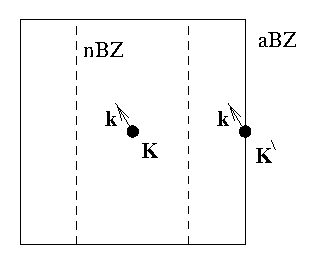
\includegraphics{2d_bz.2.eps}
\end{figure}
%


%%%
%%% Vollst"andigkeit und Orthogonalit"at der \basis 
%%%

Die Funktionen $\basis(\vec{r})$ stellen eine geeignete Basis dar,
da sie vollst"andig und orthonormal sind.

Um die Vollst"andigkeit zu zeigen, verwenden wir, da"s die Bloch-Zust"ande
(\ref{eq:bloch}) eine vollst"andige Basis bilden, d.~h.\ jede Funktion
$f(\vec{r})$ kann nach  Bloch-Zust"anden entwickelt werden 
%
\begin{eqnarray*}
  f(\vec{r}) & = & \sum_{n} \bzint{aBZ} \vdx{\akb} 
        g_{n}(\ak) e^{i\sprod{\ak}{r}} u_{n\ak}(\vec{r}) \\
  & = & \sum_{\set \,n} \: \bzint{nBZ} \vdx{\nkb}
  \underbrace{g_{n}(\nk+\set)}_{\Ts =: g_{n}^{\set}(\nk)} 
  e^{i\sprod{\nk}{r}} \underbrace{e^{i\sprod{\set}{r}}
  u_{n\vec{\nk+\set}}(\vec{r})}_{\mbox{periodisch in nEZ}}.
\end{eqnarray*}
%
Da die beiden letzten Terme periodisch in nEZ sind, k"onnen wir sie nach den
periodischen Funktionen $e^{i\sprod{\set}{r}} u_{n\vec{\set}}$
entwickeln
%
\begin{displaymath}
  e^{i\sprod{\set}{r}} u_{n \nk+\set} = \sum_{\pri{\set}\,\pri{n}}
  b^{\set \pri{\set}}_{n \pri{n}} \! (\nk) \,
  e^{i\sprod{\pri{\set}}{r}} u_{\pri{n} \vec{\pri{\set}}} ,
\end{displaymath}
%
mit den Entwicklungskoeffizienten $b^{\set \pri{\set}}_{n \pri{n}} \! (\nk)$. 
Damit ergibt sich:
%
\begin{displaymath}
  f(\vec{r}) = \sum_{\set \,n} \: \bzint{nBZ} \vdx{\nkb}
  \tilde{g}_{n}^{\set}(\nk) \basis 
  \qquad \mbox{mit} \quad
  \tilde{g}_{n}^{\set}(\nk) = \sum_{\pri{\set}\,\pri{n}}
  b^{\pri{\set} \set}_{\pri{n} n} \! (\nk) \,
  g_{\pri{n}}^{\pri{\set}}(\nk) 
\end{displaymath}
%
Wir sind also in der Lage jede beliebige Funktion $f(\vec{r})$ nach den
Basisfunktionen \basis\ zu entwickeln, was bedeutet, da"s diese vollst"andig
sind. 

Als n"achstes wollen wir die Orthonormalit"at der Basisfunktionen \basis\
zeigen, die durch die folgende Relation ausgedr"uckt wird:
%
\begin{equation}
  \label{eq:orth1}
  \bzint{Kristall}\!\!\!\! \vdx{r} \cc{{\basis}} \pbasis =
  \kronecker{\set}{\pri{\set}} \kronecker{n}{\pri{n}}
  \delta(\nk-\pri{\nk}) 
\end{equation}
%
Da"s dies erf"ullt ist, zeigt sich folgenderma"sen:
%
\begin{eqnarray}
  \label{eq:orth2}
  \bzint{Kristall}\!\!\!\! \vdx{r} \cc{{\basis}}\pbasis & = & 
  \bzint{Kristall}\!\!\!\! \vdx{r} e^{i\sprod{(\pri{k}-k)}{r}}
  \underbrace{e^{i\sprod{(\pri{\set}-\set)}{r}}
  \cc{u_{n\set}}u_{\pri{n}\pri{\set}}}_{\mbox{periodisch in nEZ}} \nonumber \\
  &=& (2\pi)^{3} \sum_{m} \BnnKK{m} \delta(\pri{\nk}-\nk-\nG) \nonumber \\
  &=& (2\pi)^{3} \BnnKK{0} \delta(\vec{\nk}-\nk)
\end{eqnarray}
%
Der letzte Schritt ist richtig, da \nk\ und \pri{\nk} aus der neuen
Brillouin-Zone sind, die durch die \{\nG\} definiert ist. Dabei haben wir eine
Fourier-Trans"-for"-mation durchgef"uhrt
%
\begin{equation}
  \label{eq:bloch-Gm}
  e^{i\sprod{(\pri{\set}-\set)}{r}} \cc{u_{n\set}}u_{\pri{n}\pri{\set}} = 
  \sum_{m} \BnnKK{m} e^{-i\sprod{\nG}{r}}
\end{equation}
%
deren Koeffizienten \BnnKK{m} durch
%
\begin{displaymath}
%  \label{eq:BnnKKm}
  \BnnKK{m} = \frac{1}{\Omega} \bzint{nEZ} \vdx{r}
  e^{i\sprod{\nG}{r}} e^{i\sprod{(\pri{\set}-\set)}{r}}
  \cc{u_{n\set}}u_{\pri{n}\pri{\set}} 
\end{displaymath}
%
gegeben sind, wenn $\Omega$ das Volumen der neuen Einheitszelle ist.
F"ur den Spezialfall $m=0$ gilt
%
\begin{equation}
  \label{eq:BnnKK0}
  \BnnKK{0} = \frac{1}{\Omega} \bzint{nEZ} \vdx{r}
  e^{i\sprod{(\pri{\set}-\set)}{r}} \cc{u_{n\set}}u_{\pri{n}\pri{\set}} =
  \frac{1}{(2\pi)^{3}} \kronecker{\set}{\pri{\set}}
  \kronecker{n}{\pri{n}}
\end{equation}
%
so da"s insgesamt Gl.~\eqref{eq:orth1} erf"ullt ist.

Gl.~\eqref{eq:BnnKK0} ist ein Spezialfall von
%
\begin{equation}
  \label{eq:K.period}
  \bzint{nEZ}e^{i\sprod{k}{r}}f(\vec{r})\vdx{r}=0
\end{equation}
%
f"ur Funktionen $f(\vec{r})$, die periodisch auf aEZ sind, und
$e^{i\sprod{k}{r}}$ periodisch auf nEZ aber nicht auf aEZ, d.~h.\  wenn
$\vec{k} \notin \{\aG\}$ gilt. 
Dies wiederum ist nur ein Spezialfall der allgemeinen Aussage, da"s
%
\begin{displaymath}
  \bzint{Kristall}e^{i\sprod{k}{r}}f(\vec{r})\vdx{r}=0 
\end{displaymath}
f"ur gitterperiodische Funktionen $f(\vec{r})$, wenn $\vec{k}$ kein reziproker
Gittervektor ist.

%%%%%%%%%%%%%%%%%%%%%%%%%%%%%%%%%%%%%%%%%%%%%%%%%%%%%%%%%%%%%%%%%%%%%%%
%%%
%%% Ansatz f"ur die Wellenfunktion
%%%
\section{Ansatz f"ur die Wellenfunktion}
\label{sec:ansatz}

Nachdem gezeigt wurde, da"s unsere Basisfunktionen \basis\ eine geeignete
Basis f"ur die Entwicklung der Eigenfunktionen 
$\psi$ in Gl.~\eqref{eq:h0+h1} sind, soll nun der Ansatz gemacht werden:
%
\begin{displaymath}
%  \label{eq:ansatz}
  \psi = \sum_{\pri{\set},\pri{n}} \bzint{nBZ} \vdx{\pri{\nkb}} \pkoeff
  \pbasis .
\end{displaymath}
%
Wenn wir dies in Gl.~\eqref{eq:h0+h1} einsetzen, so ergibt sich
%
\begin{equation}
  \label{eq:pre-SG}
  \sum_{\pri{\set},\pri{n}} \bzint{nBZ} \vdx{\pri{\nkb}}
  \matrixel{\varbasis}{\op{H_{0}}+\op{H_{1}}}{\pvarbasis} \pkoeff = E \koeff .
\end{equation}
%
Dabei steht \matrixel{\varbasis}{\op{H_{0}}+\op{H_{1}}}{\pvarbasis} f"ur
Matrixelemente bez"uglich der Basisfunktionen $\basis(\vec{r}) =
\braket{\vec{r}}{\varbasis}$. 

%%%%%%%%%%%%%%%%%%%%%%%%%%%%%%%%%%%%%
%%% Matrixelemente von $\op{H_0}$
\subsection{Matrixelemente von \op{H_0}}
\label{sec:h0}

Zun"achst sollen die Matrixelemente von \op{H_{0}} bez"uglich der
Basisfunktionen \basis\ untersucht werden.
%
\begin{equationarray*}{l}
  \matrixel{\varbasis}{\op{H_{0}}}{\pvarbasis}\\
%%%
  \;\; =\bzint{Kristall}\!\!\!\! \vdx{r} e^{-i\sprod{(\nk+\set)}{r}}
  \cc{u_{n\set}} \op{H_{0}} e^{i\sprod{(\pri{\nk}+\pri{\set})}{r}}
  u_{\pri{n}\pri{\set}}\\%[1.3ex]
%%%
  \;\; =\bzint{Kristall}\!\!\!\! \vdx{r} e^{i\sprod{(\pri{\nk}-\nk)}{r}}
  e^{-i\sprod{\set}{r}} \cc{u_{n\set}} 
  (\op{H_{0}} + \frac{\hbar^{2}}{2m} {\pri{\nkb}}^{2} 
  + \frac{\hbar}{m}\sprod{\pri{\nk}}{\op{p}}) e^{i\sprod{\pri{\set}}{r}}
  u_{\pri{n}\pri{\set}}\\%[1.3ex]
%%%
  \;\; =\bzint{Kristall}\!\!\!\! \vdx{r} e^{i\sprod{(\pri{\nk}-\nk)}{r}}
  \underbrace{e^{-i\sprod{\set}{r}} \cc{u_{n\set}} \left(
  \veps_{\pri{n}}(\pri{\set}) + \frac{\hbar^{2}}{2m} {\pri{\nkb}}^{2} +
  \frac{\hbar}{m} \sprod{\pri{\nk}}{\op{p}} \right)
  e^{i\sprod{\pri{\set}}{r}} u_{\pri{n}\pri{\set}}}_{\mbox{periodisch in nEZ}}.
\end{equationarray*}
%
Auf Grund der Periodizit"at in nEZ k"onnen wir "ahnlich wie beim Schritt von
Gl.~\eqref{eq:orth1} zu Gl.~\eqref{eq:orth2} vorgehen. Damit erhalten wir:
%
\begin{equationarray}{l}
\label{eq:preh0}
  \matrixel{\varbasis}{\op{H_{0}}}{\pvarbasis} \nonumber \\[1.5ex]
%%%%
  \;\; =\: \delta(\pri{\nk}-\nk) {\frac{(2\pi)}{\Omega}}^{3} \!\!\!
  \bzint{nEZ}\! \vdx{r} e^{-i\sprod{\set}{r}} \cc{u_{n\set}}
  \left( \veps_{\pri{n}}(\pri{\set}) + \frac{\hbar^{2}}{2m} {\nkb}^{2} +
  \frac{\hbar}{m} \sprod{\nk}{\op{p}} \right) 
  e^{i\sprod{\pri{\set}}{r}} u_{\pri{n}\pri{\set}} \nonumber \\%[1.3ex]
%%%%
  \;\; =\: \delta(\pri{\nk}-\nk) \bigg[ \kronecker{n}{\pri{n}}
  \kronecker{\set}{\pri{\set}} \left( \veps_{n}(\set) 
    + \frac{\hbar^{2}}{2m} \nkb^{2} \right) \nonumber \\%[1.3ex]
%%%%
  \qquad + \: {\frac{(2\pi)}{\Omega}}^{3} \frac{\hbar}{m}
  \bzint{nEZ} \vdx{r} 
  e^{-i\sprod{\set}{r}} \cc{u_{n\set}}  \sprod{\nk}{\op{p}}  
  e^{i\sprod{\pri{\set}}{r}} u_{\pri{n}\pri{\set}}   \bigg] 
\end{equationarray}
%
Der zweite Summand in Gl.~\eqref{eq:preh0} ergibt
%
\begin{equationarray*}{l}
  {\frac{(2\pi)}{\Omega}}^{3} \frac{\hbar}{m} \bzint{nEZ} \vdx{r}
  e^{-i\sprod{\set}{r}} \cc{u_{n\set}} \sprod{\nk}{\op{p}}  
  e^{i\sprod{\pri{\set}}{r}} u_{\pri{n}\pri{\set}} \\
%%%%
  \quad =\: \kronecker{n}{\pri{n}} \kronecker{\set}{\pri{\set}}
  \frac{\hbar}{m} \sprod{\nk}{\set} + {\frac{(2\pi)}{\Omega}}^{3}
  \frac{\hbar}{m} \bzint{nEZ} \vdx{r} e^{i\sprod{(\pri{\set}-\set)}{r}}
  \underbrace{\cc{u_{n\set}} \sprod{\nk}{\op{p}}
  u_{\pri{n}\pri{\set}}}_{\mbox{periodisch in  aEZ}}\\
%%%%
  \quad =\: \kronecker{\set}{\pri{\set}} \frac{\hbar}{m} 
  \left( \kronecker{n}{\pri{n}} \sprod{\nk}{\set} +
  {\frac{(2\pi)}{\Omega}}^{3} \bzint{nEZ}  
  \vdx{r}  \cc{u_{n\set}} \sprod{\nk}{\op{p}} u_{\pri{n}\set} \right) ,
\end{equationarray*}
%
wobei im letzten Schritt Gl.~\eqref{eq:K.period} angewendet wurde.

Es ergeben sich also keine Impulsmatrixelemente zwischen Zust"anden
verschiedener Entwicklungspunkte {\set}. In Anologie zu Gl.~\eqref{eq:pnn}
definieren wir nun:
%
\begin{equation}
  \label{eq:pnnK}
  \pnnK := {\frac{(2\pi)}{\Omega}}^{3} \bzint{nEZ} \vdx{r}
  e^{-i\sprod{\set}{r}} \cc{u_{n\set}} \, \op{\vec{p}}  \,
  e^{i\sprod{\set}{r}} u_{\pri{n}\set}
\end{equation}
%
Damit ergibt sich aus Gl.~\eqref{eq:preh0}:
%
\begin{equation}
  \label{eq:h0}
  \matrixel{\varbasis}{\op{H_{0}}}{\pvarbasis} 
  = \delta(\pri{\nk}-\nk) \kronecker{\set}{\pri{\set}} \left[
  \kronecker{n}{\pri{n}} \left( \veps_{n}(\set) + \frac{k^{2}}{2m}
  \right) + \frac{\sprod{k}{\pnnK}}{m} \right]
\end{equation}
%
Dies entspricht (nat"urlich) dem Ergebnis, das wir in Standard \kdotp-Theorie
f"ur den Punkt \set\ erhalten w"urden, wenn wir uns nur auf einen
Entwicklungspunkt im reziproken Raum beschr"ankt h"atten. Aus
Gl.~\eqref{eq:h0} l"a"st sich also direkt Gl.~\eqref{eq:standard-k.p} ableiten.
Dabei ist nicht nur die Form der Gleichung die selbe, sondern
auch die auftretenden Impulsmatrixelemente sind identisch, da das gr"o"sere
Normierungsvolumen $\Omega$ den Effekt des gr"o"seren Integrationsbereichs nEZ
wieder aufhebt.


%%%%%%%%%%%%%%%%%%%%%%%%%%%%%%%%%%%%%%%%
%%% Matrixelemente von \op{H_1}
\subsection{Matrixelemente von \op{H_1}}
\label{sec:h1}

Die Matrixelemente des St"orpotentials \op{H_{1}} bez"uglich der
Basisfunktionen \basis\ ergeben sich folgenderma"sen:
%
\begin{equation}
  \label{eq:h1mat}
  \matrixel{\varbasis}{\op{H_{1}}}{\pvarbasis} = 
  \bzint{Kristall}\!\!\!\! \vdx{r} e^{-i\sprod{(\nk+\set)}{r}}
  \cc{u_{n\set}} \op{H_{1}} e^{i\sprod{(\pri{\nk}+\pri{\set})}{r}}
  u_{\pri{n}\pri{\set}}
\end{equation}
%
Da \op{H_{1}} ein Potential und damit multiplikativ ist, vertauscht es mit
allen "ubrigen Faktoren innerhalb des Integrals \eqref{eq:h1mat}. Dadurch
ergibt sich der 
gleiche Faktor wie auf der linken Seite von Gl.~\eqref{eq:bloch-Gm}, so da"s
Gl.~\eqref{eq:h1mat} sich mit der Fourier-Entwicklung \eqref{eq:h1-Gm} als
%
\begin{eqnarray*}
%  \label{eq:preh1}
  \matrixel{\varbasis}{\op{H_{1}}}{\pvarbasis} 
  &=&  \sum_{m,\pri{m}} \BnnKK{m} \rho_{\pri{m}} 
  \bzint{Kristall}\!\!\!\! \vdx{r} e^{i\sprod{(\pri{\nk}-\nk)}{r}}
  e^{i\sprod{(\pnG-\nG)}{r}} \nonumber \\
  &=& (2\pi)^{3} \sum_{m,\pri{m}} \BnnKK{m} \rho_{\pri{m}} 
  \delta(\pnG - \pnG + \pri{\nk} - \nk) \nonumber \\
  &=& (2\pi)^{3}  \delta(\pri{\nk} - \nk) 
  \sum_{m,\pri{m}} \BnnKK{m} \rho_{\pri{m}} \kronecker{m}{\pri{m}}
\end{eqnarray*}
%
schreiben l"a"st. Der letzte Schritt ist m"oglich, da \nk\ und
\pri{\nk} aus nBZ sind, zu der die $\{\nG\}$ als reziproke
Gittervektoren geh"oren.
Hier bietet es sich an
%
\begin{eqnarray}
  \label{eq:VnnKK}
  \VnnKK &:=&  (2\pi)^{3} \sum_{m,\pri{m}} \BnnKK{m} \rho_{\pri{m}}
  \kronecker{m}{\pri{m}} \nonumber \\
  &=& {\frac{(2\pi)}{\Omega}}^{3} \bzint{nEZ} \vdx{r}
  e^{-i\sprod{\set}{r}} \cc{u_{n\set}} \op{H_{1}}  
  e^{i\sprod{\pri{\set}}{r}} u_{\pri{n}\pri{\set}}
\end{eqnarray}
%
zu definieren, so da"s wir insgesamt
%
\begin{equation}
  \label{eq:h1}
  \matrixel{\varbasis}{\op{H_{1}}}{\pvarbasis} = 
  \delta(\pri{\nk}-\nk) \VnnKK
\end{equation}
%
erhalten.

Setzen wir nun Gln.~\eqref{eq:h0} und \eqref{eq:h1} in Gl.~\eqref{eq:pre-SG}
ein, so erhalten wir als letztendlich zu l"osende Gleichung:
%
\begin{eqnarray}
  \label{eq:SG}
  \left( \veps_{n}(\set) + \frac{\hbar^{2}}{2m} \nkb^{2} \right) \koeff &+& 
  \frac{\hbar}{m} \sum_{\pri{n}} \sprod{\nk}{\pnnK} A^{\set}_{\pri{n}} \!
  (\nk) \,  \nonumber \\
%%%%
  &+& \sum_{\pri{n},\pri{\set}}  \VnnKK A^{\pri{\set}}_{\pri{n}} \!
  (\nk) \,  = E(\nk) \koeff
\end{eqnarray}
%

Es ist auffallend, da"s Gl.~\eqref{eq:SG} diagonal in \nk\ ist, weshalb sich
die Energieeigenwerte $E(\nk)$ wieder nach dem Kristallimpuls \nk\ 
klassifizieren lassen, d.~h.\ es ergibt sich wiederum eine Bandstruktur. Dies
unterscheidet sich von dem, was Luttinger und Kohn \cite{luko:55} bei der
Ableitung der EFA erhielten, die dieser Herleitung als Vorbild diente. Doch
ist dies einfach dadurch zu erkl"aren, da"s hier von einer periodischen
St"orung \eqref{eq:K.period} ausgegangen wurde und damit -- bei geeigneter
Wahl der Entwicklungspunkte im reziproken Raum -- auch ihre Matrixelemente
diagonal in \nk\ sind.\footnote{Die hier gezeigt Ableitung ist so allgemein
  gehalten, da"s sie auch f"ur nicht strengperiodische St"orungen anwendbar
  ist. So z.~B.\ St"orungen mit periodisch angeordneten Gau"s-Funktionen
  anstelle der Deltafunktionen als Fourier-Transformierte.}

%%%%%%%%%%%%%%%%%%%%%%%%%%%%%%%%%%%%%%%%%%%%%%%%%%%%%%%%%%%%%%%%%%%
%%%
%%% Diskussion
%%%
\section{Diskussion}
\label{sec:disk}

Als erstes ist festzustellen, da"s sich Gl.~\eqref{eq:SG} auf die
normale \kdotp-Gleichung \eqref{eq:standard-k.p} reduziert, wenn alle \VnnKK\ 
verschwinden und nur ein Entwicklungspunkt \set\ herangezogen wird. Schreiben
wir Gl.~\eqref{eq:SG} f"ur nichtverschwindende \VnnKK\ und zwei
Entwicklungspunkte in Matrixform, so erhalten wir eine Matrix der Form

\begin{displaymath}
\left(
  \begin{array}{c|c}
    \begin{minipage}[t][\Matrixform][c]{\Matrixform}
      \begin{center}
        Standard \kdotp-Matrix f"ur\\
        \set\ als Entwicklungspunkt + \VnnKKee
      \end{center}
    \end{minipage}&
    \begin{minipage}[t][\Matrixform][c]{\Matrixform}
      \begin{center}
        \VnnKK
      \end{center}
    \end{minipage}\\
    \hline
    \begin{minipage}[t][\Matrixform][c]{\Matrixform}
      \begin{center}
        \VnnKKze
      \end{center}
    \end{minipage}&
    \begin{minipage}[t][\Matrixform][c]{\Matrixform}
      \begin{center}
        Standard \kdotp-Matrix f"ur\\ 
        \pri\set\ als Entwicklungspunkt + \VnnKKzz
      \end{center}
    \end{minipage}
  \end{array}
\right)
\end{displaymath}
%
f"ur den Hamilton-Operator $\op{H_{0}}+\op{H_{1}}$ in der Basis der \basis.
Dabei stellt jeder der obigen Quadranten eine unendlich-dimensionale Matrix
dar, da es zu jedem Punkt im reziproken Raum unendlich viele L"osungen der
ungest"orten Schr"odingergleichung \eqref{eq:ungestoert} gibt, und damit auch
unendlich viele Basisfunktionen \basis\ zu jedem Entwicklungspunkt \set.

Insgesamt ist es also gelungen, die Differentialgleichung \eqref{eq:h0+h1} auf
die algebraische Gleichung \eqref{eq:SG} zur"uckzuf"uhren. Da hierf"ur ein
vollst"andiges Orthonormalsystem von Zust"anden verwendet wurde, ist
Gl.~\eqref{eq:SG} "aquivalent zu Gl.~\eqref{eq:h0+h1}. Dies ist vergleichbar
zu der in Kap.~\ref{sec:standard-k.p} gezeigten Situation in normaler
\kdotp-Theorie, wo auch ein differentielles Problem auf ein
unendlich-dimensionales algebraisches Problem zur"uckgef"uhrt wird
\cite{kane:66}.  Dieses unendlich dimensionale Problem k"onnen wir wieder mit
Hilfe der L"owdin-St"orungstheorie auf ein endlich-dimensionales Problem
reduzieren, wenn wir die Basisfunktionen \basis\ in zwei Gruppen zerlegen
k"onnen, wie in Kap.~\ref{sec:standard-k.p} skizziert.

%%%%%%%%%%%%%%%%%%%%%%%%%%%%%%%%%%%%
\subsection{M"ogliche Erweiterungen}
\label{sec:erweiterungen}

Da Gl.~\eqref{eq:SG} formal gro"se "Ahnlichkeit mit der Standard
\kdotp-Gleichung \eqref{eq:standard-k.p} aufweist, sind die in
Kap.~\ref{sec:standard-k.p} erw"ahnten Erweiterungen auch hier m"oglich.

So ist es sinnvoll, die Spin-Bahn-Wechselwirkung \eqref{eq:Spin-Bahn} als
zus"atzlichen Term im Hamilton-Operator zu ber"ucksichtigen, wenn die
Dispersion im Valenzband beschrieben weden soll. Es bietet sich an, diesen
Term wiederum st"orungstheoretisch zu behandeln, da sich dann die Anzahl der
notwendigen Impulsmatrixelemente \pnnK\ und Potentialmatrixelemente \VnnKK\ 
nicht erh"oht.  F"ur die Wechselwirkung mit anderen Zust"anden m"ussen wir
analog zu Kap.~\ref{sec:standard-k.p} von \pnnK\ zu
$\grvec{\pi}^{\set}_{\mathnormal{n\pri{n}}}$ "ubergehen, die sich in ihrer
Definition darin unterscheiden, da"s in Gl.~\eqref{eq:pnnK} \vecop{p} durch
$\vecop{p} + \frac{\hbar}{4mc^{2}} (\grvecop{\sigma} \times \nabla\op{V})$
ersetzt werden mu"s \cite{luko:55}.

Da in Gl.~\eqref{eq:Spin-Bahn} der Gradient des Kristallpotentials \op{V}
auftritt, stellt sich die Frage, ob das St"orpotential \op{H_{1}} hier
ber"ucksichtigt werden mu"s. Normalerweise ist dies nicht zu erwarten, da die
Spin-Bahn-Wechselwirkung auf Grund des St"orpotential \op{H_{1}} eine St"orung
h"oherer Ordnung darstellt. Falls die St"orung \op{H_{1}} aber (teilweise)
durch Relaxationen hervorgerufen wird, so ist es vorstellbar, da"s \op{H_{1}}
zwar klein ist, die Gradienten von \op{H_{1}} aber vergleichbar zu denen des
Kristallpotentials sind.

Weiterhin k"onnen auch die Methoden von Bir und Pikus \cite{bipi:74} zur
Ber"ucksichtigung von Verzerrungen durch externen Druck im Rahmen unserer
Theorie angewendet werden. Auch der Schritt von Standard \kdotp-Theorie zur
EFA l"a"st sich verallgemeinern, so da"s auch der Einflu"s flacher St"orstellen
oder Magnetfelder untersucht werden kann. Dabei k"onnen wir dem Vorgehen von
Luttinger und Kohn \cite{luko:55} folgen, da die von uns gew"ahlte Basis
\eqref{eq:basis} sehr "ahnlich zu der Basis ist, die sie verwendeten. F"ur
St"orstellen k"onnte es dabei m"oglich sein, nicht"aquivalente Einbaupl"atze
zu unterscheiden.

%%%%%%%%%%%%%%%%%%%%%%%%%%%%%%%%%%%%%%%%%%%%
\subsection{Vergleich mit anderen Methoden}
\label{sec:vergleich}

Eine "ahnliche Methode zur Ber"ucksichtigung der Mischung von Zust"anden von
verschiedenen Punkten des reziproken Raumes im Rahmen von \kdotp\ bzw.\ EFA
hat Foreman \cite{fore:98-2} vorgeschlagen. Er geht dabei unmittelbar von
einer gr"o"seren Einheitszelle aus, die der hier verwendeten nEZ entspricht.
Bez"uglich der mit dieser Einheitszelle verbundenen Brillouin-Zone geh"oren
alle Blochzust"ande, die hier zur Basis beitragen, zu \emph{einem} Punkt des
reziproken Raumes. Damit entf"allt der in Kap.~\ref{sec:basis} gef"uhrte
Beweis der Vollst"andigkeit und Orthonormalit"at und normale
\kdotp-Gleichungen k"onnen f"ur das ungest"orte Problem verwendet werden. F"ur
die durch das St"orpotential induzierten Wechselwirkungen -- bei Foreman das
Potential eines einzelnen Hetero"ubergangs zwischen AlAs und GaAs -- ergeben
sich dann Matrixelemente zwischen Blochzust"anden an \emph{einem} Punkt des
reziproken Gitters. 

Dieser Ansatz ist im wesentlichen "aquivalent zu dem hier
gew"ahlten.  Allerdings geht die Blockdiagonal-Form des Hamilton-Operators
bez"uglich der \kdotp-Wechselwirkung zun"achst verloren. Der
\kdotp-Hamilton-Operator f"ur die gr"o"sere Einheitszelle enth"alt zun"achst
Impulsmatrixelemente, deren Verschwinden erst aus einer zus"atzlichen
Betrachtung folgt. Vergleichbar zu den hier erhaltenen Ergebnissen w"urde sich
bei einer solchen Betrachtung auch ergeben, da"s die tats"achlich ben"otigten
Impulsmatrixelemente die gleichen sind, wie sie in einer \kdotp-Rechnung f"ur
den ungest"orten Kristalls in seiner primitiven Einheitszelle ben"otigt
werden, wenn alle \{\set\} unabh"angig voneinander als Entwicklungspunkte
verwendet werden. Dies ist deshalb von Vorteil, da der ungest"orte Kristall im
Allgemeinen eine h"ohere Symmetrie aufweist, so da"s aus gruppentheoretischen
Gr"unden insgesamt weniger unabh"angige Parameter zu ber"ucksichtigen sind.

Bei dem Problem der Mischung von Blochzust"anden wie es Foreman betrachtet,
spielt dies nur eine untergeordnete Rolle. Doch hier sollen auch
Energiedispersionen berechnet werden, und da ist diese Reduzierung der Anzahl
der unabh"angigen Paramter wichtig. 

Das f"ur die Berechnung der Energiedispersionen verwendete Verfahren weist
"Ahnlichkeiten mit Methoden auf, die auf Cardona zur"uckgehen \cite{card:63}.
Dabei werden die Impulsmatrixelemente in Halbleitern mit Zinkblende-Gitter auf
entsprechenden Matrixelemente isoelektrischer Halbleiter mit Diamant-Gitter
zur"uckgef"uhrt.\footnote{D.~h.  da"s z.~B.\ Impulsmatrixelemente f"ur GaAs
  auf die in Ge zur"uckgef"uhrt werden.}  Das inversions-asymmetrische
Potential, das den Unterschied zwischen Zinkblende- und Diamant-Struktur
beschreibt, wird dazu als St"orung eines zugrundeliegenden Diamant-Gitters
aufgefa"st.  Die Blochzust"ande der polaren Materialien k"onnen dadurch als
"Uberlagerung von Zu"-st"an"-den eines unpolaren Materials dargestellt werden.
Damit ergeben sich auch die Impulsmatrixelemente aus "Uberlagerungen der
Impulsmatrixelemente des unpolaren Materials. Im Diamant-Gitter gibt es aber
auf Grund der h"oheren Symmetrie weniger unabh"angige Parameter, so da"s auf
diesem Weg unbekannte Impulsmatrixelemente der Zinkblende-Struktur durch
bekannte Energieunterschiede und Impulsmatrixelemente des isoelektrischen
Diamant-Gitters ausgedr"uckt werden k"onnen. Der wesentliche Unterschied zu
dem hier behandelten Problem besteht darin, da"s das von Cardona verwendete
St"orpotential das Bravais-Gitter des Kristalls nicht "andert, so da"s keine
Mischung von Zust"anden verschiedener Punkte im \vec{k}-Raum auftritt. 
Zudem ist es in diesem Fall ausreichend, nur \emph{ein} Impulsmatrixelement und
\emph{ein} Potentialmatrixelement zu ber"ucksichtigen, was das Problem
deutlich vereinfacht.


%. Dadurch sind keine
%relativen Phasen zu beachtet, was nicht immer einfach ist, wie wir in
%Kap.~\ref{sec:phase} sehen werden. Wie dieses Problem sowie die nicht-triviale
%Bestimmung der \VnnKK behandelt werden kann, soll nun im n"achsten Kapitel
%gezeigt werden.

%%% local Variables: 
%%% mode: latex
%%% TeX-master: "diplom"
%%% End: 



% Anwendung auf GaInP
%%% Kapitel "uber die Anwendung 'meiner' k.p Methode auf geordnetes GaInP
%%% Time-stamp: <1999-03-04 11:50:00 ralf>

%%%%%%%%%%%%%%%%%%%%%%%%%%%%%%%%%%%%%%%%%%%%%%%%%%%%%%%%%%%%%%
%%%%%%%%%%%%%%%%%%%%%%%%%%%%%%%%%%%%%%%%%%%%%%%%%%%%%%%%%%%%%%
%%%%
%%%%
\chapter{Anwendung auf geordnetes \GaInP}
\label{cha:anwend}

In diesem Kapitel soll gezeigt werden, wie sich die in
Kap.~\ref{cha:period-stoer} abgeleitete Theorie auf ein konkretes Problem, die
effektive Masse der Elektronen im Leitungsband von (teil-)geordnetem \GaInP,
anwenden l"a"st.

%%%%%%%%%%%%%%%%%%%%%%%%%%%%%%%%%%%%%%%%%%%%%%%%%%%%%%%%%%%%%%
%%%%
\section{Allgemeines zum Materialsystem}
\label{sec:materialsystem}

Viele III--V-Halbleiterlegierungen $A_{x}B_{1-x}C$ mit Kationen $A$ und $B$
zeigen spontane, langreichweitige \CuPt-Ordnung, wenn sie mit
metallorganischer Gasphasen-Epitaxie [\emph{metalorganic vapour phase epitaxy}
(MOVPE)] auf $(001)$-orientierten Substraten gewachsen werden \cite{zuma:94}.
Die geordnete Phase besteht aus abwechselnden Monolagen
$A_{x+\eta/2}B_{1-x-\eta/2}C$ und $A_{x-\eta/2}B_{1-x+\eta/2}C$, die l"angs
der $[111]$-Richtung angeordnet sind. Dabei ist $0 \le \eta \le 1$ der
Ordnungsgrad. Die $[111]$-Richtung wird als Ordnungsrichtung
bezeichnet.\footnote{Im Prinzip w"are auch eine der drei Richtungen m"oglich,
  die zur $[111]$-Richtung "aquivalent sind. Doch hat dies hier keinerlei
  Auswirkungen, so da"s wir hier bei nur einer Richtung bleiben wollen.}

Ein prominentes Beispiel f"ur diese Materialien ist
Ga$_{x}$In$_{1-x}$P. Mit \GaInP\ wollen wir den Fall $x \approx 0.5$
bezeichnen, der gitterangepa"st auf GaAs Substraten aufgewachsen werden kann
\cite{kipp:97}. Ein Vergleich der mikroskopischen Struktur der ungeordneten
Zinkblende-Struktur und einem \CuPt-geordneten Material ist in
Abb.~\ref{fig:ZnS-CuPt} zu sehen.

\begin{figure}[hbtp]
  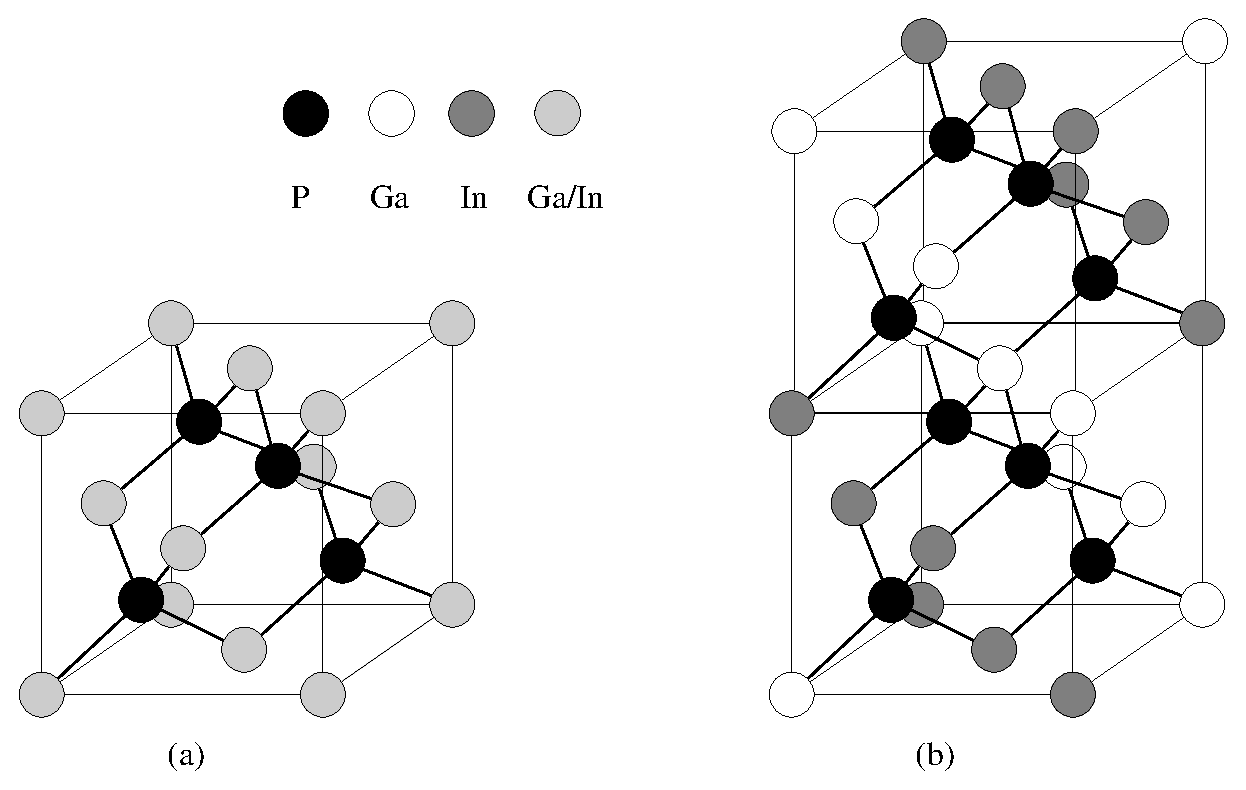
\includegraphics[width=\textwidth]{zns.eps}
  \caption{Vergleich der mikroskopischen Struktur in einem (a)
    Zinkblende-Gitter mit einem (b) vollst"andig \CuPt-geordneten Material.}
  \label{fig:ZnS-CuPt}
\end{figure}

Abb.~\ref{fig:ZnS-CuPt}(b) zeigt den Fall idealer Ordnung, d.~h.\
Ordnungsgrad $\eta=1$. Allerdings wurden im Experiment bisher nur teilgeordnete
Proben gefunden. Das bedeutet $\eta < 1$, so da"s auf  aufeinanderfolgenden
$(111)$-Ebenen die \emph{Wahrscheinlichkeit} abwechselnd erh"oht (erniedrigt)
und erniedrigt (erh"oht) ist, ein Ga (In) Atom zu finden. Dabei h"angt der
Ordnungsgrad von verschiedenen Wachstumsbedingungen wie Temperatur und
Substratorientierung ab.

%\begin{floatingfigure}{50mm}
%  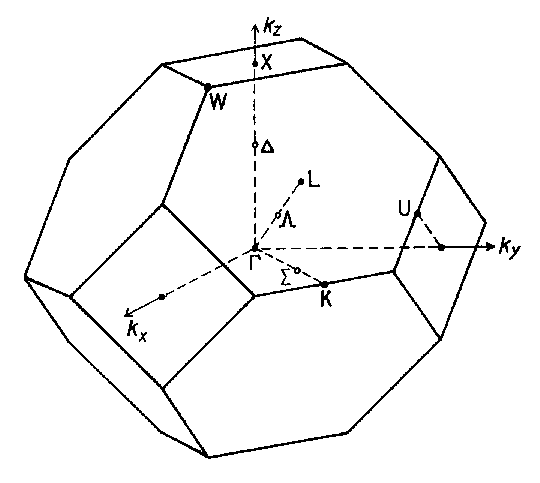
\includegraphics[width=40mm]{bz-fcc.eps}
%  \caption{Brillouin Zone eines Zinkblende Kristalls}
%  \label{fig:bz-fcc}
%\end{floatingfigure}


\begin{floatingfigure}{75mm}
  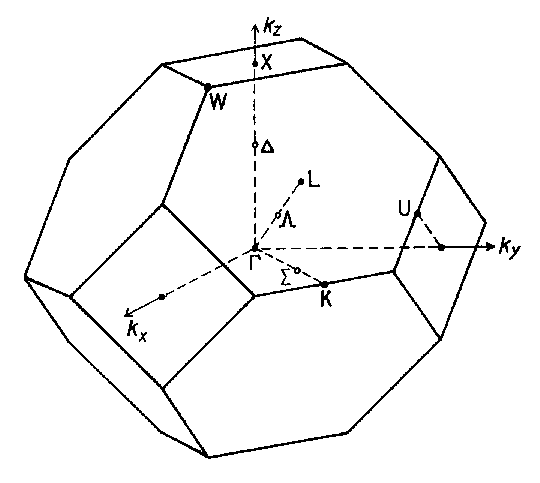
\includegraphics[width=65mm]{bz-fcc.eps}
  \caption{Brillouin Zone eines Kristalls mit Zinkblende-Struktur}
  \label{fig:bz-fcc}
\end{floatingfigure}


\sloppy 
Beim "Ubergang vom unge"-ordneten ($\eta=0$) Zinkblende-System zu einem
\CuPt-ge"-ordneten Kristall wird die Einheitszelle verdoppelt und damit die
Brillouin-Zone halbiert. Die Punktgruppe des Kristalls reduziert sich von \Td\ 
zu \Cdv.\footnote{Die Bezeichnungen von Punktgruppen und derer (irreduziblen)
  Darstellungen folgt der Notation von Koster \emph{et al.}  \cite{kdws:63}.}
Diese Verkleinerung der Brillouin-Zone bewirkt ein Zur"uckfalten von
Zust"anden. An jedem Punkt der neuen Brillouin-Zone finden sich Zust"ande, die
sich urspr"unglich an zwei verschiedenen Punkten der Brillouin-Zone des
Zinkblende-Gitters befanden. Die f"ur uns interessanten Zust"ande befinden
sich im Zentrum der neuen Brillouin-Zone.  Der eine Teil der dort zu findenden
Zust"ande war auch im Zinkblende-Gitter schon am $\Gamma$-Punkt. Der andere
Teil faltet von dem L-Punkt zur"uck, der in Ordnungsrichtung
liegt.\footnote{Den vier prinzipiell m"oglichen Ordnungsrichtungen entsprechen
  auch vier L-Punkte.}
%Der Satz \set\ an Punkten im reziproken Raum umfa"st hier also den $\Gamma$-
%und den L-Punkt.

\fussy

Dies f"uhrt zu einer ganzen Reihe von Effekten, von denen wir die wichtigsten
hier behandeln wollen. Zwei der auff"alligsten  
sind die Reduzierung der Bandl"ucke um $\Delta E_{\text{BGR}}$ und die
Kristallfeldaufspaltung $\Delta_{\text{CF}}$. Letzteres bedeutet, da"s das ohne
Spin-Bahn-Wechselwirkung dreifach entartete \GVB-Valenzband"-maximum in einen
zweifach entarteten $\bGVB{3} (\GVB)$-Zustand und einen einfach entarteten
$\bGVB{1} (\GVB)$-Zustand aufspaltet.\footnote{Bei der Notation der Zust"ande
  in der teilgeordneten Phase, folgen wir hier der z.~B.\ in
  Ref.~\cite{wfz:95} zu findenden. Dabei wird die Symmetrie eines Zustandes im
  \CuPt-geordneten Kristall mit einem Strich versehen, w"ahrend die Symmetrie
  desjenigen Zinkblende-Zustands der ma"sgeblich beitr"agt in Klammern
  angegeben wird. Die Zuordnung der Zinkblende-Zust"ande ist
  Abb.~\ref{fig:band-short} zu entnehmen.}

%\begin{figure}[htb]
%  \begin{minipage}[c]{50mm}
%    \caption{Brillouin-Zone eines Kristalls mit Zinkblende-Struktur}
%    \label{fig:bz-fcc}
%  \end{minipage}
%  \hfill
%  \begin{minipage}[c]{70mm}
%    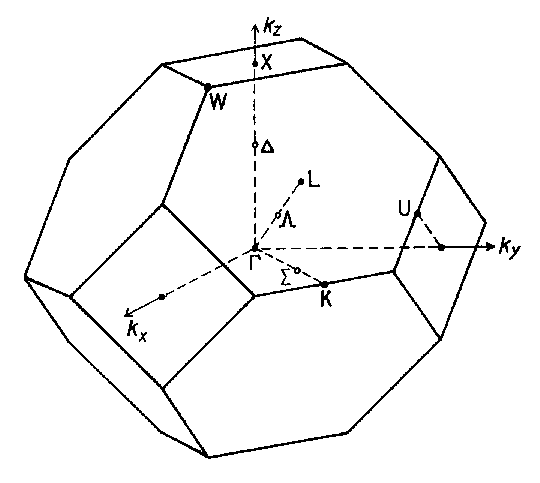
\includegraphics[width=70mm]{bz-fcc.eps}
%  \end{minipage}
%\end{figure}

Wird die Spin-Bahn-Wech"-sel"-wirkung ber"ucksichtigt, so zeigt sich die
Kristallfeldaufspaltung in einer Aufhebung der vierfachen Entartung des
$\Gamma_{\text{8v}}$ Valenzbandes. Die sich hier ergebende Aufspaltung
entspricht \emph{nicht} der Kristallfeldaufspaltung. Aus der
Valenzbandaufspaltung l"a"st sich aber die Kristallfeldaufspaltung berechnen,
wenn f"ur die Spin-Bahn-Wechselwirkung die quasikubische N"aherung gemacht
wird \cite{bipi:74}, bei der eine von der Symmetrie her m"ogliche Anisotropie
in der Spin-Bahn-Wechselwirkung vernachl"assigt wird. 

Theoretische Vorhersagen \cite{wezu:98} und Messungen \cite{fzcm:97,fgmz:98}
haben gezeigt, da"s zwischen Bandl"uckenreduzierung $\Delta E_{\text{BGR}}$ und
Kristallfeldaufspaltung $\Delta_{\text{CF}}$ eine vom Ordnungsgrad
unabh"angige Beziehung herrscht. F"ur \GaInP\ finden diese Autoren
%
\begin{equation}
  \label{eq:zeta}
  \zeta_{\text{theo}} = \frac{\Delta E_{\text{BGR}}}{\Delta_{\text{CF}}} = 2,69
  \quad \text{bzw.} \quad \zeta_{\text{exp}} \approx 2,65 .
\end{equation}
%

Weiterhin sind in (teil-)geordnetem \GaInP\ optische "Uberg"ange m"oglich, die
im ungeordneten Fall dipolverboten sind. Einer von diesen ist der "Ubergang
$\bGVB{3}(\GVB) \rightarrow \bGCB (\LCB)$, der vor kurzem genauer
untersucht wurde \cite{kksk:99}. Tr"agt man die "Ubergangsenergie als Funktion der
Bandl"uckenreduzierung auf, so ergibt sich eine Gerade mit Steigung
$\theta = 0,48$. Es besteht also ein eindeutiger Zusammenhang zwischen dem
Ordnungsgrad, repr"asentiert durch die Bandl"uckenreduzierung $\Delta
E_{\text{BGR}}$, und der "Anderung $\Delta E_{\Gamma \rightarrow \text{L}}$
der Energie des "Ubergang $\bGVB{3}(\GVB) \rightarrow \bGCB (\LCB)$, gegeben
durch 
%
\begin{equation}
  \label{eq:theta}
  \theta = \frac{\Delta E_{\Gamma \rightarrow \text{L}}}
  {\Delta E_{\text{BGR}}} = 0,48 .
\end{equation}
%
%Diese beiden Zahlen werden in Kap.~\ref{sec:betrag} wichtig sein,
%wenn es darum geht, den Betrag von Matrixelementen zu bestimmen.


%%%%%%%%%%%%%%%%%%%%%%%%%%%%%%%%%%%%%%%%%%%%%%%%%%%%%%%%%%%%%%
%%%%
\section{Beschreibung der effektiven Massen im Leitungsband}
\label{sec:k.p-m-CB}

Die bisher erw"ahnten Untersuchungen besch"aftigten sich nur mit den Energien
verschiedener Zust"ande in Abh"angigkeit vom Ordnungsgrad, d.~h.\ mit
statischen Eigenschaften. Eine wichtige Gr"o"se bei der Beschreibung
dynamischer Eigenschaften -- z.~B.\ Transportph"anomenen -- sind die
effektiven Massen der Elektronen im Valenz- und Leitungsband.
%\marginpar{Etwas "uber die Definition
%  der effektiven Masse???}

Als erste versuchten Raikh und Tsiper \cite{rats:94}, die effektive Masse im
Leitungsband "uber die Kopplung zwischen den B"andern \GCB\ und \LCB\ im
Rahmen einer Effektive-Massen-N"aherung zu beschreiben. Das unbekannte
Matrixelement f"ur diese Kopplung pa"sten sie dabei an beobachtete
Bandl"uckenreduzierungen an, da \LCB\ energetisch h"oher liegt als \GCB\ und
die Kopplung zu einer Absto"sung dieser Zust"ande f"uhrt. Au"serdem mischen
die Zust"ande auf Grund dieser Kopplung. Da die effektiven Massen von \LCB\ 
anisotrop und gr"o"ser als bei \GCB\ sind, ergibt sich mit diesem Modell die
Vorhersage eines Anstiegs der effektiven Masse im untersten Leitungsband als
Funktion des Ordnungsgrades.  Dabei sollte der Anstieg parallel zur
Ordnungsrichtung gr"o"ser sein als senkrecht zu ihr, also
$m^{\ast}_{\parallel} > m^{\ast}_{\perp} > m^{\ast}_{\text{c}}$. Hier
bezeichnet $m^{\ast}_{\text{c}}$ die isotrope effektive Masse von \GCB,
$m^{\ast}_{\parallel}$ die effektive Masse parallel zur Ordnungsrichtung und
$m^{\ast}_{\perp}$ die effektive Masse senkrecht zur Ordnungsrichtung.

Problematisch bei diesem Ansatz ist, da"s die Bandl"uckenreduzierung zu einer
Verst"arkung der Wechselwirkung zwischen Valenzbandmaximum und
Leitungsbandminimum f"uhrt, was eine \emph{Reduzierung} der effektiven Masse
im Leitungsband zur Folge hat. Dies wurde von Zhang und Mascarenhas
\cite{zhma:95} untersucht. Ausgehend von einem acht B"ander
($\Gamma_{\text{6c}}, \Gamma_{\text{8v}}, \Gamma_{\text{7v}}$) umfassenden
\kdotp-Hamilton-Operator f"ur den ungeordneten Kristall, ber"ucksichtigten sie
die Ordnungseffekte durch zwei Parameter, welche die Bandl"uckenreduzierung
und Kristallfeldaufspaltung beschreiben.\footnote{Tats"achlich f"uhren sie
  zun"achst mehr Parameter ein, deren Form sich aus Symmetrie"uberlegungen
  ergibt, vernachl"assigen dann aber die "Ubrigen.}  Sie erhielten damit eine
reduzierte effektive Masse im Leitungsband. Bedingt durch die
Kristallfeldaufspaltung im Valenzband fiel diese in Ordnungsrichtung
schw"acher aus, also $m^{\ast}_{\text{c}} > m^{\ast}_{\parallel} >
m^{\ast}_{\perp}$.

In diesem Ansatz fehlen aber die Effekte der $\Gamma$--L-Mischung, die
nicht vernachl"assigbar sind. Franceschetti, Wei und Zunger \cite{fwz:95}
zeigten dies, indem sie \emph{ab initio} Bandstruktur-Rechnungen
(Dichtefunktionaltheorie in lokaler Dichten"aherung) f"ur den ideal
geordneten Fall durchf"uhrten. Dabei fanden sie $m^{\ast}_{\parallel} >
m^{\ast}_{\perp}$, in "Ubereinstimmung mit obigen Rechnungen. Aber die
effektive Masse im ungeordneten Material befand sich zwischen diesen beiden
Werten, also $m^{\ast}_{\parallel} > m^{\ast}_{\text{c}} > m^{\ast}_{\perp}$.
Die Schlu"sfolgerung der Autoren war, da"s die effektive Masse der
Leitungsbandelektronen empfindlich davon abh"angt, in welchem Verh"altnis
$\Gamma$--L-Mischung und verst"arkte Kopplung zum Valenzband zueinander
stehen.

Sowohl die $\Gamma$--L-Mischung, als auch die verst"arkte Kopplung zum
Valenzband beruhen beide auf der Wechselwirkung zwischen Zinkblende
$\Gamma$- und L-Zust"anden. Ein Modell, das diese Wechselwirkung richtig
beschreibt, sollte deshalb auch in der Lage sein, die Ordnungsabh"angigkeit
der effektiven Masse im Leitungsband korrekt zu beschreiben. Ein solches
Modell ist mit der in Kap.~\ref{cha:period-stoer} abgeleiteten Theorie
m"oglich, und wir wollen sie nun auf dieses Problem anwenden.


%%%%%%%%%%%%%%%%%%%%%%%%%%%%%%%%%%%%%%%%
\subsection{Wahl der Basisfunktionen}
\label{sec:basiswahl}

Das ungest"orte Problem von dem wir ausgehen wollen ist der ungeordnete
Kristall, beschrieben durch den Hamilton-Operator \op{H_{0}}. F"ur diesen
ben"otigen wir als Parameter die Energieeigenwerte $\veps_{n}(\vec{k})$ und
die Impulsmatrixelemente \pnnK\ aus Gl.~\eqref{eq:h0}. Dazu f"uhren wir eine
Bandstruktur-Rechnung durch und beschreiben dabei den ungeordneten Kristall
mit der N"aherung eines virtuellen Kristalls [\emph{virtual crystal
  approximation} (VCA)]. F"ur diese Berechnung verwenden wir die Methode der
Linearkombination atomarer Orbitale [\emph{linear combination of atomic
  orbitals} (LCAO), oft auch \emph{tight-binding approximation} (TBA)
genannt]. Dabei bleibt die Spin-Bahn-Wechselwirkung unber"ucksichtigt. Die
Spin-Bahn-Aufspaltung ist mit einem Betrag von etwa 100~meV verglichen mit
einer Bandl"ucke von 1.97~eV nicht vernachl"assigbar, doch ist der Einflu"s
der Spin-Bahn-Aufspaltung auf die effektive Masse im Leitungsband sehr gering.
Auf Details dieser Rechnung werden wir in Anhang \ref{cha:lcao} eingehen.
Ergebnisse sind z.~B.\ in Abb.~\ref{fig:band-short} dargestellt.

\begin{figure}[htb]
  \includegraphics[width=\textwidth]{band-short.eps}
  \caption{Bandstruktur in ungeordnetem \GaInP}
  \label{fig:band-short}
\end{figure}


Die St"orung \op{H_{1}} entspricht dem Unterschied zwischen dem
Kristallpotential im (teil-)geordneten und ungeordneten Fall. Dieses
Ordnungspotential\footnote{Dieser Begriff wurde zuerst von Wei und Zunger
  \cite{wezu:89} eingef"uhrt.}  
hat nicht mehr die Symmetrie des Zinkblende-Gitters (Punktgruppe \Td) sondern
die der geordneten Phase, f"ur die \CuPt-Struktur also Punktgruppe \Cdv.
Deshalb ist es in der Lage, Zust"ande verschiedener Symmetrie im
Zinkblende-Gitter zu koppeln, wenn sie in der \CuPt-geordneten Struktur die
gleiche Symmetrie haben. Dabei wollen wir nur Kopplungen zwischen Zust"anden
ber"ucksichtigen, die zu verschiedenen \vec{k}-Punkten im Zinkblende-Kristall
geh"oren, aber nach der Faltung am gleichen \vec{k}-Punkt zu finden sind. Das
bedeutet, da"s in der Entwicklung \eqref{eq:h1-Gm} nur diejenigen
Koeffizienten $\rho_{m}$ ber"ucksichtigt werden, die zu \emph{neuen}
reziproken Gittervektoren \nG\ geh"oren, aber nicht die, die zu alten
reziproken Gittervektoren \aG\ geh"oren. Raikh und Tsiper
\cite{rats:94} haben gezeigt, da"s dies im Rahmen der VCA exakt gilt, wenn im
geordneten Kristall keine Relaxationen auftreten. Experimente, welche das Ma"s
an Relaxation untersuchten, wurden bisher nicht ver"offentlicht.  Theoretische
Untersuchungen \cite{wfz:95,ylcy:97} lassen keinen eindeutigen Schlu"s zu,
ob Relaxationen notwendig sind oder nicht, um beobachtete Gr"o"sen wie z.~B.\ 
die Kristallfeldaufspaltung zu erkl"aren. Allerdings stimmen sie darin
"uberein, da"s Relaxationen auch die Kopplung zwischen Zust"anden von
verschiedenen \vec{k}-Punkten der Zinkblende-Brillouin-Zone verst"arken
w"urden, so da"s es gerechtfertigt erscheint, die Matrixelemente zwischen
Zust"anden vom gleichen \vec{k}-Punkt zu vernachl"assigen. F"ur die in
Kap.~\ref{sec:disk} skizzierte Matrixform des Hamilton-Operators hei"st dies,
da"s die \VnnKKee\ und \VnnKKzz\ nicht ber"ucksichtigt werden.

Wie in Kap.~\ref{sec:basis} gezeigt, sind die Zust"ande von $\Gamma$- und
L-Punkt, die hier den Satz \{\set\} aus Kap.~\ref{sec:basis} bilden,
ein vollst"andiges Orthonormalsystem. Doch ist das sich daraus ergebende
unendlich-dimensionale Gleichungssystem f"ur praktische Rechnungen nicht
praktikabel, weshalb die Einschr"ankung auf eine geeignete Basis ein wichtiger
Schritt ist. Die kleinste Basis, die es noch erm"oglicht die
wesentlichen physikalischen Vorg"ange zu beschreiben, enth"alt die Zust"ande
\GCB, \GVB, \LCB\ und \LVB\ (siehe Abb.~\ref{fig:band-short}). Zwischen den
Leitungsbandzust"anden ist auf Grund des geringen Energieabstandes eine starke
Wechselwirkung zu erwarten. Die Mischung dieser Zust"ande beeinflu"st die
effektiven Massen im Leitungsband unmittelbar. Zus"atzlich reduziert sich noch
die Bandl"ucke, was die \kdotp-Wechselwirkung mit dem Valenzband verst"arkt.
Um dies zu beschreiben, reicht es aber nicht aus, nur die \GVB-Zust"ande zu
ber"ucksichtigen, da die Kristallfeldaufspaltung zu einer Anisotropie in der
\kdotp-Wechselwirkung zwischen Valenz- und Leitungsband f"uhrt. Die
Kristallfeldaufspaltung k"onnen wir aber nur "uber die Wechselwirkung zwischen
\GVB- und \LVB-Zust"anden erkl"aren, so da"s die \LVB-Zust"ande auch in die
Basis aufgenommen werden m"ussen.



%%%%%%%%%%%%%%%%%%%%%%%%%%%%%%%%%%%%%%%%
\subsection{Der \kdotp-Hamilton-Operator}
\label{sec:k.p-H}

Die Form des \kdotp-Hamilton-Operators, der zur Basis aus
Kap.~\ref{sec:basiswahl} geh"ort, l"a"st sich aus allgemeinen
gruppentheoretischen "Uberlegungen ableiten. Dabei wollen wir zun"achst die
Standard \kdotp\ Teile betrachten.

Der \kdotp-Hamilton-Operator f"ur \GCB\ und \GVB\ ist wohlbekannt.
Vernachl"assigen wir das Fehlen von Inversionssymmetrie und w"ahlen $x$, $y$
und $z$ entlang der kubischen Kristallachsen $[100]$, $[010]$ und $[001]$, so
ist er durch 
%Gl.~\eqref{eq:k.p-G} 
%
%\setcounter{floateq}{\value{equation}}
%\begin{floateq}
\vspace*{4ex}
\begin{equation}
\renewcommand{\arraystretch}{1.6}
\setlength{\arraycolsep}{0.5ex}
\label{eq:k.p-G}
\op{H_{\Gamma}} = 
\left(
\begin{array}{c|ccc}
  \raisebox{2.0em}[0ex][0ex]{\ket{\GCB}} 
& \raisebox{2.0em}[0ex][0ex]{\ket{\GVBx}} 
& \raisebox{2.0em}[0ex][0ex]{\ket{\GVBy}} 
& \raisebox{2.0em}[0ex][0ex]{\ket{\GVBz}} \\[-4ex]
%%%%%%%%%%% 
\begin{array}[c]{c}
 E_{\Gamma\text{c}} + \frac{\hbar^{2}}{2m} k^{2} \\ + \pri{A} k^{2}  
\end{array}
&  i\PG k_{x} 
&  i\PG k_{y} 
&  i\PG k_{z} \\
%%%%%%%%%%%
\hline
  -i\cc{\PG} k_{x} 
& \begin{array}[c]{c}
  \frac{\hbar^{2}}{2m} k^{2} + \pri{L} k_{x}^{2} \\ 
  + \pri{M} (k_{y}^{2}+k_{z}^{2})
\end{array}
& \pri{N} k_{x} k_{y} 
& \pri{N} k_{x} k_{z} \\
%%%%%%%%%%%
  -i\cc{\PG} k_{y} 
& \pri{N} k_{x} k_{y} 
& \begin{array}[c]{c}
  \frac{\hbar^{2}}{2m} k^{2} + \pri{L} k_{y}^{2} \\ 
  + \pri{M} (k_{x}^{2}+k_{z}^{2})
\end{array}
& \pri{N} k_{y} k_{z} \\
%%%%%%%%%%%
  -i\cc{\PG} k_{z} 
& \pri{N} k_{x} k_{z} 
& \pri{N} k_{y} k_{z} 
& \begin{array}[c]{c}
  \frac{\hbar^{2}}{2m} k^{2} + \pri{L} k_{z}^{2} \\ 
  + \pri{M} (k_{x}^{2}+k_{y}^{2})
\end{array} \\
\end{array}\right) 
\renewcommand{\arraystretch}{0.625}
\end{equation}
%\end{floateq}
%
gegeben \cite{kane:66}, wobei $\pri{A}$, $\pri{L}$, $\pri{M}$ und $\pri{N}$
die Wechselwirkung mit energetisch weiter entfernten B"andern repr"asentieren,
die "uber L"owdin-St"orungstheorie \cite{lowd:51} ber"ucksichtigt wurde; $m$
ist die Masse des freien Elektrons. Das reduzierte Impulsmatrixelement \PG\ 
ist gegeben durch
%
\begin{displaymath}
  \PG = - i \frac{\hbar}{m} \matrixel{\GCB}{\op{p_{x}}}{\GVBx}.
\end{displaymath}
%
Dieses Matrixelement bezieht sich dabei auf ein Integral "uber die
Einheitszelle von ungeordnetem \GaInP\ von der Form \eqref{eq:pnnK}. Dort
entspricht der Integrationsbereich zwar der Einheitszelle von geordnetem
\GaInP, doch wie bereits in Kap.~\ref{sec:h0} erw"ahnt, h"angt der Wert des
Impulsmatrixelements nicht vom Integrationsbereich ab, da sich das auftretende
Normierungsvolumen entsprechend "andert.

Der Hamilton-Operator f"ur das \LVB-Band ist z.~B.\ bei Bir und
Pikus~\cite{bipi:74} zu finden, wobei wiederum Terme linear in \vec{k}, die
von der Inversionsasymmetrie des Zinkblende-Gitters herr"uhren,
vernachl"assigt werden. Wir wollen aber die Wechselwirkung mit \LCB\ explizit
ber"ucksichtigen, so da"s wir untersuchen m"ussen, welche Impulsmatrixelemente
zwischen diesen Zust"anden existieren. W"ahlen wir die $z$-Achse parallel zur
$[111]$-Richtung, so transformiert sich die $z$-Komponente des Impulsoperators
gem"a"s der irreduziblen Darstellung \IRREP{1} von \Cdv, $x$- und
$y$-Komponente wie \IRREP{3}. Das Wigner-Eckart-Theorem zusammen mit den bei
Koster \emph{et al.} \cite{kdws:63} tabellierten Clebsch-Gordan-Koeffizienten
ergibt nun, da"s es am L-Punkt, "ahnlich wie am $\Gamma$-Punkt, nur ein
reduziertes Impulsmatrixelement innerhalb der von uns gew"ahlten Basis gibt.
Im Unterschied zum $\Gamma$-Punkt gibt es aber keine Kopplung in $z$-Richtung,
da $\matrixel{\LCB}{\op{p}_{z}}{\LVB} = 0 $ gilt.\footnote{In der Sprache der
  Gruppentheorie hei"st das, da"s \IRREP{1} nicht in der Produktdarstellung
  $\IRREP{1} \otimes \IRREP{3}$ enthalten ist.}  Somit erhalten wir
%Gl.~\eqref{eq:k.p-L}
%
%\setcounter{floateq}{\value{equation}}
%\begin{floateq}
  \vspace*{4ex}
\begin{equation}
\label{eq:k.p-L}
\renewcommand{\arraystretch}{1.6}
\setlength{\arraycolsep}{0.5ex}
\op{H_{\text{L}}} = \left(
\begin{array}{c|cc}
  \raisebox{2.0em}[0ex][0ex]{\ket{\LCB}} 
& \raisebox{2.0em}[0ex][0ex]{\ket{\LVBx}} 
& \raisebox{2.0em}[0ex][0ex]{\ket{\LVBy}} \\[-4ex]
%%%%%%%%%%%
\begin{array}[c]{c}
  E_{\text{Lc}} + \frac{\hbar^{2}}{2m} k^{2} \\ 
  + F k_{\perp}^{2} + G k_{z}^{2} 
\end{array}
& i\PL k_{x} 
& i\PL k_{y} \\
\hline
%%%%%%%%%%%
  -i\cc{\PL} k_{x} 
& \begin{array}[c]{c}
  E_{\text{Lv}} + \frac{\hbar^{2}}{2m} k^{2} + A k_{z}^{2} \\
  + B (k_{x}^{2}+k_{y}^{2}) + C k_{y} k_{z}
\end{array}
& C k_{x} k_{z} \\
%%%%%%%%%%%
  -i\cc{\PL} k_{y} 
& C k_{x} k_{z} 
& \begin{array}[c]{c}
  E_{\text{Lv}} + \frac{\hbar^{2}}{2m} k^{2} + A k_{z}^{2} \\ 
  + B (k_{x}^{2}+k_{y}^{2}) + C k_{y} k_{z}
\end{array}\\
\end{array}\right),
\renewcommand{\arraystretch}{0.625}
\end{equation}
%\end{floateq}
%
wobei $A$, $B$, $C$, $F$ und $G$ die Wechselwirkung mit energetisch weiter
entfernten B"andern beschreiben. Das reduzierte Impulsmatrixelement \PL\ ist
gegeben durch
%
\begin{displaymath}
  \PL =  - i \frac{\hbar}{m} \matrixel{\LCB}{\op{p_{x}}}{\LVBx}.
\end{displaymath}
%
Dabei wurde neben $\ez \parallel [111]$ noch $\ex \parallel [1 \bar{1} 0]$ und
$\ey \parallel [1 1 \bar{2}]$ gew"ahlt. Da dann $x$ in einer Spiegelebene von
\Cdv\ liegt, $y$ dagegen senkrecht zu dieser steht, erkl"art dies die
$x$-$y$-Asymmetrie in Gl.~\eqref{eq:k.p-L}.
 
\begin{figure}[htb]
  \includegraphics[width=\textwidth]{band-long.eps}
  \caption{Bandstruktur in ungeordnetem \GaInP. Senkrecht zur $[111]$-Richtung
    ist die Dispersion am L-Punkt qualitativ "ahnlich zu der am
    $\Gamma$-Punkt.} 
  \label{fig:band-long}
\end{figure}

Damit wir bei der Bestimmung der m"oglichen Potentialmatrixelemente das
Wigner-Eckart-Theorem effektiv anwenden k"onnen, m"ussen wir
Gl.~\eqref{eq:k.p-G} im gleichen Koordinatensystem wie Gl.~\eqref{eq:k.p-L}
schreiben. Da wir hier nicht versuchen wollen, die Dispersion der
Valenzb"ander zu beschreiben, brauchen wir die Parameter $\pri{L}$, $\pri{M}$
und $\pri{N}$ in Gl.~\eqref{eq:k.p-G} nicht zu ber"ucksichtigen, wodurch die
n"otige Drehung des Koordinatensystems f"ur die Hamilton-Matrix
\eqref{eq:k.p-G} trivial wird. Aus den selben Gr"unden k"onnen wir auch $A$,
$B$ und $C$ in Gl.~\eqref{eq:k.p-L} vernachl"assigen. 

Es ist bekannt, da"s im Zentrum der Brillouin-Zone die effektive Masse des
untersten Leitungsbandes zum gr"o"sten Teil "uber die Wechselwirkung mit dem
Valenzbandmaximum erkl"art werden kann. Dabei stammt der zweitgr"o"ste Anteil
von der Wechselwirkung mit dem untersten sich nach \IRREP{5} transformierenden
Leitungsband. Das mit dieser Wechselwirkung assoziierte Matrixelement
\pri{\PG} (siehe Abb.~\ref{fig:short+V_P}) betr"agt aber etwa $0.35 \PG$
\cite{ccf:88} und soll deshalb hier vernachl"assigt werden. Wir w"ahlen also
$\pri{A}=0$ in der Hamilton-Matrix \eqref{eq:k.p-G}.

In Abb.~\ref{fig:band-long} ist zu sehen, da"s die Dispersion am L-Punkt
\emph{senkrecht} zur $[111]$-Richtung qualitativ "ahnlich zu der am
$\Gamma$-Punkt ist. Auch die Beziehung zwischen \pri{\PL} und \PL\ ist
vergleichbar zu der von \pri{\PG} und \PG, wie Cardona zeigen konnte
\cite{card:63}. Deshalb wollen wir auch diesen Fernbandbeitrag
vernachl"assigen und damit in Gl.~\eqref{eq:k.p-L} $F=0$ w"ahlen.

\renewcommand{\bottomfraction}{0.7}
%
\begin{figure}[hb]
  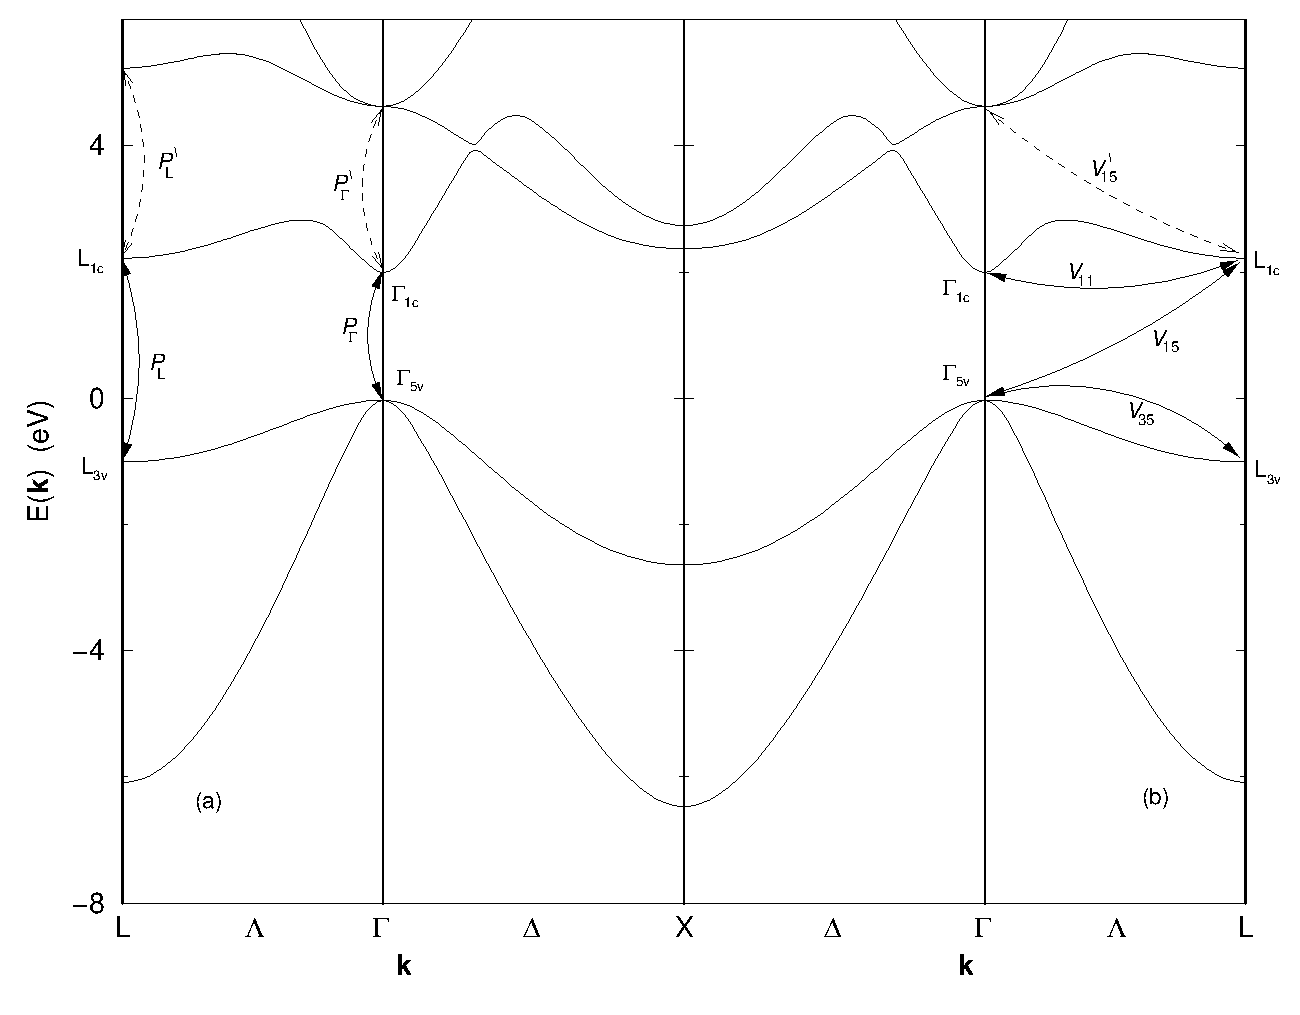
\includegraphics[width=\textwidth]{short+V_P.eps}
  \caption{Bandstruktur in  ungeordnetem GaInP mit (a) \kdotp- und (b)
      Potential-Matrixelementen.} 
  \label{fig:short+V_P}
\end{figure}
%

Nur die Dispersion am L-Punkt parallel zur $[111]$-Richtung l"a"st sich nicht
mit Wechselwirkungen innerhalb der hier gew"ahlten Basis erkl"aren. Deshalb
behalten wir $G$ als einzigen Beitrag energetisch weiter entfernter B"ander in
unserem Modell.

Die Bestimmung der m"oglichen Potentialmatrixelemente ist direkt "uber das
Wigner-Eckart Theorem m"oglich.\footnote{Da sich \op{H_{1}} gem"a"s der
  trivialen Darstellung \IRREP{1} von \Cdv\ transformiert, kann auch eine
  spezielle Form des Wigner-Eckart-Theorems verwendet werden \cite{corn:69}.
  Diese besagt, da"s dann nur Matrixelemente zwischen Zust"anden m"oglich
  sind, die sich nach der gleichen irreduziblen Darstellung
  transformieren, und die dazugeh"origen Clebsch-Gordan-Koeffizienten
  proportional zur Einsmatrix sind.}  
\LCB\ und \op{H_{1}} transformieren sich gem"a"s \IRREP{1} von \Cdv, \LVBx\ 
und \LVBy\ transformieren sich gemeinsam gem"a"s \IRREP{3}. Die
Wellenfunktionen des $\Gamma$-Punkts haben ein wohldefiniertes
Transformationsverhalten unter den Operationen von \Td. Uns interessiert aber,
wie sie sich unter Transformationen von \Cdv\ verhalten. Da \Cdv\ eine
Untergruppe der \Td\ ist, l"a"st sich diese Frage mit Hilfe der
Kompatibilit"atsrelationen beantworten, wie sie bei Koster \emph{et al.}
\cite{kdws:63} zu finden sind. Mit dem bei Gl.~\eqref{eq:k.p-L} verwendeten
Koordinatensystem erhalten wir, da"s sich \GCB\ und \GVBz\ gem"a"s \IRREP{1}
von \Cdv\ transformieren, und da"s \GVBx\ und \GVBy\ sich gemeinsam gem"a"s
\IRREP{3} von \Cdv\ transformieren. Damit ergibt sich, da"s es nur drei
verschiedene Matrixelemente zwischen den Zust"anden in unserer Basis gibt:
%
\begin{subequations}
\label{eq:def-V}
\begin{eqnarray}
\label{eq:V11,V35,V15}
  \V{11} &=& \matrixel{\GCB}{\op{H_{1}}}{\LCB}\\
  \V{35} &=& \matrixel{\GVBx}{\op{H_{1}}}{\LVBx} =
  \matrixel{\GVBy}{\op{H_{1}}}{\LVBy} \\
  \V{15} &=& \matrixel{\GVBz}{\op{H_{1}}}{\LCB}
\end{eqnarray}
\end{subequations}
%
Dabei bezieht sich das Matrixelement auf ein Integral "uber die Einheitszelle
von geordnetem \GaInP\ von der Form \eqref{eq:VnnKK}. Ordnungsbedingte
Wechselwirkungen mit Zust"anden au"serhalb der hier gew"ahlten Basis werden
wegen des gro"sen energetischen Abstands dieser Niveaus nicht ber"uchsichtigt.

Abb.~\ref{fig:short+V_P} zeigt nochmal im "Uberblick, welche Matrixelemente in
unserem Modell ber"ucksichtigt werden (durchgezogenen Linien). Als
durchbrochene Linien sind noch diejenigen Impuls- und Potentialmatrixelemente
eingezeichnet, die bei einer Verfeinerung des Modells als erste
ber"ucksichtigt werden sollten.

%
%%%%%%%%%%%% Gesamt k.p Hamilton-Operator
\begin{sidewaysfloateqnum}
\begin{equation}
\label{eq:k.p-H}
\caption{\kdotp-Hamilton-Operator inklusive Potentialmatrixelementen}
\renewcommand{\arraystretch}{1.6}
\op{H_{\Gamma \text{L}}} = \left(
\begin{array}{c|cc|c||c|cc}
  \raisebox{2.0em}[0ex][0ex]{\ket{\GCB}} 
& \raisebox{2.0em}[0ex][0ex]{\ket{\GVBx}} 
& \raisebox{2.0em}[0ex][0ex]{\ket{\GVBy}} 
& \raisebox{2.0em}[0ex][0ex]{\ket{\GVBz}} 
& \raisebox{2.0em}[0ex][0ex]{\ket{\LCB}} 
& \raisebox{2.0em}[0ex][0ex]{\ket{\LVBx}} 
& \raisebox{2.0em}[0ex][0ex]{\ket{\LVBy}} \\[-4ex]
%%%%%%%%%%%
E_{\Gamma\text{c}} + \frac{\hbar^{2}}{2m} k^{2} 
& i\PG k_{x} 
& i\PG k_{y} 
& i\PG k_{z} 
& \V{11} 
& 0 
& 0 \\
\hline
%%%%%%%%%%%
  -i\cc{\PG} k_{x} 
& \frac{\hbar^{2}}{2m}k ^{2} 
& 0 
& 0 
& 0 
& \V{35} 
& 0 \\
%%%%%%%%%%%
  -i\cc{\PG} k_{y} 
& 0 
& \frac{\hbar^{2}}{2m} k^{2} 
& 0 
& 0 
& 0 
& \V{35}   \\
%%%%%%%%%%%
\hline
  -i\cc{\PG} k_{z} 
& 0 
& 0 
& \frac{\hbar^{2}}{2m} k^{2} 
& \V{15} 
& 0 
& 0 \\
\hline\hline
%%%%%%%%%%%
\cc{\V{11}} 
& 0 
& 0 
& \cc{\V{15}} 
& \begin{array}[c]{c} E_{\text{Lc}} + \frac{\hbar^{2}}{2m} k^{2}\\
  + G k_{z}^{2}
  \end{array} 
& i\PL k_{x} 
& i\PL k_{y}\\
%%%%%%%%%%%
\hline
0 
& \cc{\V{35}} 
& 0 
& 0 
& -i\cc{\PL} k_{x} 
& E_{\text{Lv}} + \frac{\hbar^{2}}{2m} k^{2} 
& 0 \\
%%%%%%%%%%%
0 
& 0 
& \cc{\V{35}} 
& 0 
& -i\cc{\PL} k_{y} 
& 0 
& E_{\text{Lv}} + \frac{\hbar^{2}}{2m} k^{2} \\
\end{array} \right)
\renewcommand{\arraystretch}{0.625}
\end{equation}
\end{sidewaysfloateqnum}
%
Fassen wir nun Gln.~\eqref{eq:k.p-G} und \eqref{eq:k.p-L} mit diesem Ergebnis
zusammen, so erhalten wir als Hamilton-Operator Gl.~\eqref{eq:k.p-H} (siehe
S.~\pageref{eq:k.p-H}). Dabei haben wir die oben genannten N"aherungen
bez"uglich der Fernbandbeitr"age bereits ber"ucksichtigt.

%%%%%%%%%%%%%%%%%%%%%%%%%
% Betrag und Phase der Matrixelemente

%%%%%%%%%%%%%%%%%%%%%%%%%%%%%%%%%%%%%%%%%%%%%%%%%%%%%%%%%%%%%%
%%%%
\section{Bestimmung der Matrixelemente}
\label{sec:ME}

Um Gl.~\eqref{eq:k.p-H} l"osen zu k"onnen, ist es notwendig, die in ihr
vorkommenden Matrixelemente zu bestimmen. Eine wichtige Voraussetzung dazu
ist, da"s wir sowohl am $\Gamma$- als auch am L-Punkt eines Zinkblende-Gitters
die Wellenfunktionen reell w"ahlen k"onnen, wenn wir -- wie hier geschehen --
keine Spin-Bahn-Wechselwirkung ber"ucksichtigen. Dieser Effekt der
Zeitumkehrsymmetrie soll im folgenden kurz erl"autert werden.

Sei $\psi_{n\vec{k}}$ eine L"osung der station"aren Schr"odinger-Gleichung,
d.~h.\ 
%
\begin{displaymath}
    \op{H} \psi_{n\vec{k}} = \veps_{n}(\vec{k})\psi_{n\vec{k}},
\end{displaymath}
%
f"ur das Problem eines Teilchens in einem periodischen Potential. In diesem
Fall gilt das Bloch-Theorem
%
\begin{equation}
  \label{eq:Bloch-Theorem}
  \psi_{n\vec{k}}(\vec{r} + \vec{R}) = e^{i\sprod{k}{R}} \psi_{n\vec{k}}(\vec{r})
\end{equation}
%
f"ur alle Gittervektoren $\vec{R}$ des periodischen Potentials. Der
Wellenvektor \vec{k} h"angt also mit der diskreten Translationsinvarianz des
Problems zusammen. Ist \op{H} zeitumkehrinvariant, so ist aber auch
$\cc{\psi}_{n\vec{k}}$ ein L"osung der station"aren Schr"odinger-Gleichung zum
gleichen Eigenwert:\footnote{Betrachtet man die (zeitabh"angige)
  Schr"odinger-Gleichung, so sieht man, da"s die komplex-konjugierte Gleichung
  als zeitumgekehrte Gleichung aufgefa"st werden kann. F"ur einen
  zeitumkehrinvarianten Hamiltonoperator gilt also $\cc{\op{H}}=\op{H}$. Die
  Eigenwerte sind reell, da \op{H} hermitesch ist.}
%
\begin{displaymath}
  \op{H} \cc{\psi}_{n\vec{k}} = \veps_{n}(\vec{k}) \cc{\psi}_{n\vec{k}}
\end{displaymath}
%
Bilden wir nun das komplex-konjugierte von Gl.~\eqref{eq:Bloch-Theorem},
so erhalten wir
%
\begin{displaymath}
  \cc{\psi}_{n\vec{k}}(\vec{r} + \vec{R}) = e^{-i\sprod{k}{R}}
  \cc{\psi}_{n\vec{k}}(\vec{r}) ,
\end{displaymath}
%
d.~h.\ $\cc{\psi}_{n\vec{k}}$ geh"ort zum Wellenvektor \vec{-k}. Am
$\Gamma$-Punkt sind aber wegen $k=0$ sowohl $\psi_{n\vec{k}}$ als auch
$\cc{\psi}_{n\vec{k}}$ am gleichen Punkt im reziproken Raum angesiedelt.
F"ur den L-Punkt mit $\vec{k} = 2\pi/a_{\text{latt}} (1/2,1/2,1/2)$ gilt das
ebenso, da $-\vec{k} = \vec{k}- \vec{G}$ mit dem reziproken Gittervektor
$\vec{G} = 2\pi/a_{\text{latt}} (1,1,1)$ gilt, und somit
%
\begin{displaymath}
  \cc{\psi}_{n\vec{k}}(\vec{r} + \vec{R}) = 
  e^{-i\sprod{k}{R}} \cc{\psi}_{n\vec{k}}(\vec{r}) =
  e^{i\sprod{(k-G)}{R}} \cc{\psi}_{n\vec{k}}(\vec{r}) =
  e^{i\sprod{k}{R}} \cc{\psi}_{n\vec{k}}(\vec{r}),
\end{displaymath}
%
wegen $\sprod{G}{R}=2\pi n$ und $n \in \mathbb{Z}$ f"ur alle Gittervektoren
\vec{G} und \vec{R} des reziproken und realen Raumes. Wenn aber sowohl
$\psi_{n\vec{k}}$ als auch $\cc{\psi}_{n\vec{k}}$ Eigenzust"ande zum gleichen
Energie-Eigenwert und zum gleichen Wellenvektor sind, so k"onnen wir immer
reelle Funktionen $\frac{1}{2}(\psi_{n\vec{k}} + \cc{\psi}_{n\vec{k}})$ und
$\frac{1}{2i}(\psi_{n\vec{k}} - \cc{\psi}_{n\vec{k}})$ verwenden. Wir k"onnen
also davon ausgehen, da"s wir es in unserer Basis nur mit reellen
Wellenfunktionen zu tun haben. Dies bedeutet aber f"ur die in \op{H_{\Gamma
\text{L}}} [Gl.~\eqref{eq:k.p-H}] auftretenden Matrixelemente, da"s sie
ebenfalls reell sind. 


%%%%%%%%%%%%%%%%%%%%%%%%%%%%%%%%%%%%%%%%
\subsection{Betrag der Matrixelemente}
\label{sec:betrag}

F"ur $\V{11} = \V{35} = \V{15} = 0$ beschreibt Gl.~\eqref{eq:k.p-H}
den ungeordneten Kristall, den wir im Rahmen der TBA modellieren (siehe
Anhang~\ref{cha:lcao}). Damit k"onnen wir aber den Betrag der
Impulsmatrixelemente \PG\ und \PL\ sowie den Fernbandbeitrag $G$ aus den
effektiven Massen berechnen, die sich in der TBA-Rechnung ergeben. Dabei ist
die effektive Masse in der Umgebung von \vec{k_{\text{0}}} eigentlich ein
Tensor zweiter Stufe: 
%
\begin{displaymath}
%  \label{eq:m*-tensor}
   \frac{1}{m^{\ast}_{\alpha\beta}} = \left. \frac{1}{\hbar^{2}}
   \frac{\partial^{2} E}{\partial k_{\alpha} \partial k_{\beta}}
   \right|_{\vec{k}=\vec{k_{\text{0}}}} 
\end{displaymath}
%
F"ur die nichtentarteten Leitungsb"ander k"onnen wir diesen Tensor aber immer
auf Hauptachsenform bringen. Im Valenzband reichen am $\Gamma$-Punkt die
effektiven Massen in $[100]$-Richtung, am L-Punkt die in $[111]$- und $[1
\bar{1} 0]$-Richtung aus, um die Impulsmatrixelemente zu berechnen. Deshalb
k"onnen wir uns auf die zweite Ableitung bez"uglich der entsprechenden
Komponenten von \vec{k} beschr"anken.
%
\begin{equation}
  \label{eq:m*-d2E/dk2}
  \frac{1}{m^{\ast}} = \left. \frac{1}{\hbar^{2}} \frac{\partial^{2}
  E}{\partial k^{2}} \right|_{\vec{k}=\vec{k_{\text{0}}}}
\end{equation}
%
Die Energiedispersion $E(\vec{k})$ ist aber nicht analytisch bekannt. Vielmehr
mu"s der entsprechende TBA-Hamilton-Operator numerisch diagonalisiert 
werden. Wir k"onnen deshalb Gl.~\eqref{eq:m*-d2E/dk2} nicht direkt verwenden,
sondern m"ussen zu einer diskretisierten Form "ubergehen. Da das hier
verwendet Modell bez"uglich der Extrema \vec{k_{\text{0}}}
inversionssymmetrische Energiedispersionen liefert, erhalten wir
%
\begin{equation}
  \label{eq:m*-diskret}
  \frac{m}{m^{\ast}} = \frac{2m}{\hbar^{2}}
  \frac{E(\vec{k}) - E(\vec{k_{\text{0}}})}
  {(\vec{k} - \vec{k_{\text{0}}})^{2}}.
\end{equation}
%
Bei der Anwendung von Gl.~\eqref{eq:m*-diskret} mu"s sichergestellt werden,
da"s zum einen $\Delta k = |\vec{k}-\vec{k_{\text{0}}}|$ nicht zu gro"s wird,
da sonst die quadratische N"aherung der Dispersion nicht mehr gilt.
Andererseits darf $\Delta E = |E(\vec{k}) - E(\vec{k_{\text{0}}})|$ nicht zu
klein sein, da sonst Fehler in der Numerik
% und Unsicherheiten in den
%empirischen Parametern, die in den TBA-Hamilton-Operator eingehen, 
zu gro"ses
Gewicht erhalten. F"ur die Berechnung wurden typischerweise Werte von $\Delta E
= 0,2 \dots 4$~meV und $\Delta k = 0,001 \dots 0,04$ in Einheiten von
$2\pi/a_{\text{latt}}$ verwendet.

Damit erhalten wir die in Tab.~\ref{tab:Em*P} (siehe S.~\pageref{tab:Em*P})
dargestellten effektiven Massen.  Dabei ist zu beachten, da"s es sich bei
$m^{\text{v}}_{\Gamma}$ und $m^{\text{v}}_{\text{L}\perp}$ jeweils um die
Masse der leichten L"ocher handelt, die zu dem st"arker gekr"ummten Band
geh"ort (siehe auch Abb.~\ref{fig:band-long}). F"ur $m^{\text{c}}_{\Gamma}$
geben Emanuelsson \emph{et al.} \cite{edhm:94} einen Wert von
$(0,092\pm0,003)m$ an, in sehr guter "Ubereinstimmung mit unserem Ergebnis.

Aus der Beziehung
%
\begin{displaymath}
  \frac{m}{m^{\text{c}}_{\text{L}\parallel}} = 1 + \frac{2m}{\hbar^{2}}G
\end{displaymath}
%
ergibt sich der Fernbandbeitrag $G = -1,57$~eV\AA$^{2}$. Um \PG\ und \PL\ zu
bestimmen, diagonalisieren wir Gl.~\eqref{eq:k.p-H} f"ur $\V{11} = \V{35} =
\V{15} = 0$ in zweiter Ordnung St"orungstheorie, und erhalten die bekannten
Beziehungen 
%
\begin{subequations}
\label{eq:m*-P}
\begin{eqnarray}
  \label{eq:m*-PGC}
  \frac{m}{m^{\text{c}}_{\Gamma}} &=&
  1+ \frac{2m}{\hbar^{2}}\frac{|\PG|^{2}}{E_{\Gamma\text{c}}}\\
  \label{eq:m*-PGV}
  \frac{m}{m^{\text{v}}_{\Gamma}} &=&
  1- \frac{2m}{\hbar^{2}}\frac{|\PG|^{2}}{E_{\Gamma\text{c}}}\\
  \label{eq:m*-PLC}
  \frac{m}{m^{\text{c}}_{\text{L}\perp}} &=&
  1+ \frac{2m}{\hbar^{2}}\frac{|\PL|^{2}}{E_{\text{Lc}}-E_{\text{Lv}}}\\
  \label{eq:m*-PLV}
  \frac{m}{m^{\text{v}}_{\text{L}\perp}} &=& 1-
  \frac{2m}{\hbar^{2}}\frac{|\PL|^{2}}{E_{\text{Lc}}-E_{\text{Lv}}},
\end{eqnarray}
\end{subequations}
%
wobei wieder das Maximum des Valenzbandes als Nullpunkt der Energieskala
gew"ahlt wurde.  Um aus diesen Gleichungen \PG\ und \PL\ zu bestimmen,
ben"otigen wir noch die Energieeigenwerte der Niveaus, die sich in unserer
Basis befinden.  Tab.~\ref{tab:Em*P} zeigt die Ergebnisse, die wir mit Hilfe
der TBA erhalten haben. L"osen wir nun Gln.~\eqref{eq:m*-P} auf und setzen die
Energieeigenwerte und effektiven Massen aus Tab.~\ref{tab:Em*P} ein, so
erhalten wir die in der rechten Spalte von Tab.~\ref{tab:Em*P} aufgef"uhrten
Werte f"ur die Impulsmatrixelemente.
%
\begin{table}[bht]
%\setlength{\tabcolsep}{0.5ex}
\renewcommand{\arraystretch}{1.6}
  \begin{center}
    \begin{tabular}{c@{\hspace{2ex}}l@{\hspace{0.6ex}}r*{2}{@{\hspace{4ex}}l@{=\hspace{0.6ex}}r}}
%    \begin{tabular}{|c|l@{\hspace{0.6ex}}r|*{2}{l@{=\hspace{0.6ex}}r|}}
\hline\hline
Zustand 
& \multicolumn{2}{c}{\hspace{-4ex}Energie} 
& \multicolumn{2}{c}{\hspace{-4ex}effektive Masse}
& \multicolumn{2}{c}{Matrixelement}\\
\hline
\GCB 
& $E_{\Gamma\text{c}} =$ & 2,024 eV 
& $m^{\text{c}}_{\Gamma}$ & 0,0899 $m$
& $|\PG|$ & 8,83 eV\AA\\[1ex]
%\hline
\GVB
& $E_{\Gamma\text{v}} =$ & 0 eV
& $m^{\text{v}}_{\Gamma}$ & -- 0,0994 $m$
& $|\PG|$ & 9,24 eV\AA\\[1ex]
%\hline
 & \multicolumn{2}{l}{}
& $m^{\text{c}}_{\text{L}\perp}$ & 0,1349 $m$
& $|\PL|$ & 8,88 eV\AA\\
%\cline{4-7}
\raisebox{2.4ex}[-2,4ex]{\LCB}
& \raisebox{2.4ex}[-2,4ex]{$E_{\text{Lc}} =$} 
& \raisebox{2.4ex}[-2,4ex]{2,250 eV}
& $m^{\text{c}}_{\text{L}\parallel}$ & 1,699 $m$
& $G$ & -- 1,57 eV\AA$^{2}$\\[1ex]
%\hline
 & \multicolumn{2}{l}{}
& $m^{\text{v}}_{\text{L}\perp}$ & -- 0,1349 $m$
& $|\PL|$ & 10,2 eV\AA\\
%\cline{4-7}
\raisebox{2.4ex}[-2.4ex]{\LVB}
& \raisebox{2.4ex}[-2.4ex]{$E_{\text{Lv}} =$} 
& \raisebox{2.4ex}[-2.4ex]{-- 0,978 eV}
&  $m^{\text{v}}_{\text{L}\parallel}$ & 2,088 $m$
& \multicolumn{2}{l}{} \\[0.5ex]
\hline \hline
    \end{tabular}
    \caption{Energie, effektive Masse und daraus bestimmtes
      Impulsmatrixelement bzw. Fernbandbeitrag f"ur die Zust"ande \GCB, \GVB,
      \LCB\ und \LVB\ in ungeordnetem \GaInP.}
    \label{tab:Em*P}
  \end{center}
\renewcommand{\arraystretch}{0.625}
\end{table}
%

Es f"allt auf, da"s unser Modell keine einheitlichen Werte f"ur die
Impulsmatrixelemente liefert. Doch lassen sich diese Unterschiede zwanglos
durch die vernachl"assigten Fernbandbeitr"age erkl"aren. Da unser
Hauptaugenmerk den Zust"anden im Leitungsband gilt, wollen wir nur die Werte
verwenden, die sich aus den effektiven Massen im Leitungsband
ergeben. Weiterhin ist auff"allig, da"s sich die damit ergebenden Werte f"ur
\PG\ und \PL\ kaum unterscheiden. Darauf hatte schon Cardona \cite{card:63}
hingewiesen, und wir wollen deshalb im weiteren
%
\begin{displaymath}
  |\PG| = |\PL| = 8.86\text{~eV\AA}
\end{displaymath}
%
verwenden.

Bei der Bestimmung der Betr"age der Potentialmatrixelemente $\V{11}$, $\V{35}$
und $\V{15}$ gehen wir ganz "ahnlich vor. Zun"achst diagonalisieren wir
Gl.~\eqref{eq:k.p-H} f"ur $k=0$ in zweiter Ordnung St"orungstheorie.
Damit erhalten wir Ausdr"ucke f"ur die Kristallfeldaufspaltung
$\Delta_{\text{CF}}$, die Bandl"uckenreduzierung $\Delta E_{\text{BGR}}$ und
die "Anderung $\Delta E_{\Gamma \rightarrow \text{L}}$ der "Ubergangsenergie
$\bGVB{3}(\GVB) \rightarrow \bGCB (\LCB)$ in Abh"angigkeit von diesen drei
Matrixelementen:
%
\begin{subequations}
\label{eq:Delta-V}
\begin{eqnarray}
  \label{eq:DeltaCF}
  \Delta_{\text{CF}} &=&
  - \frac{|\V{35}|^{2}}{E_{\text{Lv}}} + \frac{|\V{15}|^{2}}{E_{\text{Lc}}} \\
  \label{eq:DeltaEBGR}
  \Delta E_{\text{BGR}} &=&
  \frac{|\V{11}|^{2}}{E_{\text{Lc}}-E_{\Gamma\text{c}}} -
  \frac{|\V{35}|^{2}}{E_{\text{Lv}}} \\
  \label{eq:DeltaEG-L}
  \Delta E_{\Gamma \rightarrow \text{L}} &=&
  \frac{|\V{11}|^{2}}{E_{\text{Lc}}-E_{\Gamma\text{c}}} +
  \frac{|\V{15}|^{2}}{E_{\text{Lc}}} + \frac{|\V{35}|^{2}}{E_{\text{Lv}}}
\end{eqnarray}
\end{subequations}
%
Wie bereits in Kap.~\ref{sec:materialsystem} erw"ahnt, sind die Gr"o"sen
$\theta = \Delta E_{\Gamma \rightarrow \text{L}} / \Delta E_{\text{BGR}}$ und
$\zeta = \Delta E_{\text{BGR}} / \Delta_{\text{CF}}$ aus theoretischen und
experimentellen Untersuchungen bekannt. Damit sind wir in der Lage, die
Potentialmatrixelemente \V{15} und \V{35} durch \V{11}, $\theta$ und $\zeta$
auszudr"ucken:
%
\begin{subequations}
\label{eq:V-V}
\begin{eqnarray}
  \label{eq:V35-V11}
  \frac{|\V{35}|^{2}}{E_{\text{Lv}}} &=& \frac{\theta - 1 -
    \frac{1}{\zeta}}{\theta + 2 - \frac{1}{\zeta}}
  \frac{|\V{11}|^{2}}{E_{\text{Lc}}-E_{\Gamma\text{c}}} =
  - 0.426 \frac{|\V{11}|^{2}}{E_{\text{Lc}}-E_{\Gamma\text{c}}} \\
  \label{eq:V15-V11}
  \frac{|\V{15}|^{2}}{E_{\text{Lc}}} &=& \frac{\theta - 1 +
    \frac{2}{\zeta}}{\theta + 2 - \frac{1}{\zeta}}
  \frac{|\V{11}|^{2}}{E_{\text{Lc}}-E_{\Gamma\text{c}}} = \;\;\: 0.110
  \frac{|\V{11}|^{2}}{E_{\text{Lc}}-E_{\Gamma\text{c}}}
\end{eqnarray}
\end{subequations}
%
Dabei haben wir die Werte der Gln.~\eqref{eq:zeta} und \eqref{eq:theta}
eingesetzt. 

Damit haben wir als einzigen freien Parameter das Matrixelement \V{11}, das in
unserem Modell den Grad der Ordnung beschreibt. Denn je gr"o"ser der
Ordnungsgrad ist, desto st"arker ist das Ordnungspotential, so da"s auch
\V{11} betragsm"a"sig gr"o"ser wird. Modellieren wir das Ordnungspotential
"uber VCA, so ist dieses proportional zum Ordnungsgrad $\eta$ \cite{rats:94},
und damit sind nat"urlich auch die Matrixelemente proportional zum
Ordnungsrad. Dies seinerseits f"uhrt dann zu konstanten Verh"altnissen
zwischen den Potentialmatrixelementen, die unabh"angig vom Ordnungsgrad sind,
wie in Gln.~\eqref{eq:V-V}.
%\marginpar{Etwas
%  "uber Vertrauensbereich wegen s. Ord. PT, Exp. eh nur f"ur geringe Ordnung
%  \dots}


%%%%%%%%%%%%%%%%%%%%%%%%%%%%%%%%%%%%%%%%
\subsection{Phase der Matrixelemente}
\label{sec:phase}

Als letzte unbekannte Gr"o"sen in unserem Modell, m"ussen wir nun noch die
Phasen der Matrixelemente bestimmen. Es reicht dabei aus die relativen
Vorzeichen zu bestimmen, da eine gemeinsame Phase aller Matrixelemente keine
Auswirkungen auf das Ergebnis hat, und aus dem oben gezeigten folgt, da"s die
Wellenfunktionen in unserer Basis, und damit auch die Matrixelemente, reell
w"ahlbar sind.  F"ur die Potentialmatrixelemente ist dies leicht zu sehen, da
\op{H_{1}(\vec{r})} eine reelle Funktion sein mu"s. Somit sind die
Potentialmatrixelemente Integrale "uber ein Produkt reeller Funtionen und
somit auch reell. Schreiben wir den Impulsoperator in Ortsdarstellung, so
erhalten wir f"ur die Impulsmatrixelemente ein Integral "uber das Produkt
einer reellen Funktion mit der Ableitung einer reellen Funktion, was wiederum
reell ist.
%
%\begin{displaymath}
%  \label{eq:PG-Ort}
%  \PG = - i \frac{\hbar}{m} \matrixel{\GCB}{\op{p_{x}}}{\GVBx} 
%      = \frac{\hbar^{2}}{m} \matrixel{\GVBx}{\pdx{x}}{\GCB},
%\end{displaymath}
%

Das Vorzeichen von \PG\ und \PL\ h"angt von der Wahl der Phasen der Zust"ande
ab. Um diese zu bestimmen, folgen wir dem Ansatz in Ref.~\cite{ccf:88}. Aus
einer TBA-Rechnung mit einer Basis aus einem $s$-artigen und drei
$p$-artigen Wellenfunktionen pro Atom erhalten wir ein schematisches Bild der
Wellenfunktionen in unserer Basis (siehe Anhang \ref{cha:lcao}). Diese Wellenfunktionen sind in
Abb.~\ref{fig:wfkt-G} f"ur den $\Gamma$-Punkt und in Abb.~\ref{fig:wfkt-L}
f"ur den L-Punkt skizziert. Grau schattierte Bereiche geben dabei ein positives
Vorzeichen der Wellenfunktion an, wei"se Bereiche bedeuten ein negatives
Vorzeichen. Im Bild zu \GCB\ sind zus"atzlich noch die Atome gekennzeichnet.
A1 und C1 bezeichnet Anion und Kation f"ur das Zinkblende-Gitter. A2 und C2
bezeichnet die Atome, die beim "Ubergang zur \CuPt-Einheitszelle dazukommen.
Skizzieren wir nun grob die Bereiche negativer \emph{Ableitung} bez"uglich $x$
der Leitungsband-Wellenfunktionen \GCB\ und \LCB, so stellen wir fest, da"s
die Verteilung der Vorzeichen im wesentlichen der der Valenzbandzust"ande
\GVBx\ und \LVBx\ entspricht. Das bedeutet aber, da"s das Produkt aus
Valenzband-Wellenfunktion und Ableitung der Leitungsbandwellenfunktion im
wesentlichen positiv ist, und somit auch die beiden Impulsmatrixelemente f"ur
\emph{diese} Wahl der Phasen positiv sind. Somit erhalten wir:
%
\begin{displaymath}
%  \label{eq:PG=PL}
  \PG = \PL = 8.86\text{~eV\AA}
\end{displaymath}
%
 
%\begin{sidewaysfigure}
\begin{figure}
  \centering
  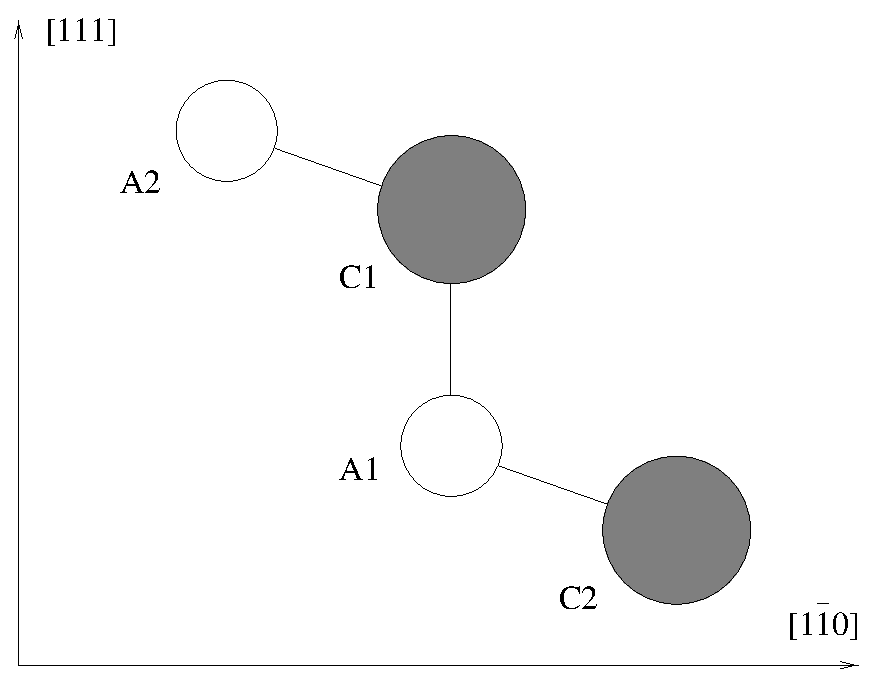
\includegraphics[width=10cm]{G1c.eps}\raisebox{4cm}{(a)}
  \vspace{2ex}
  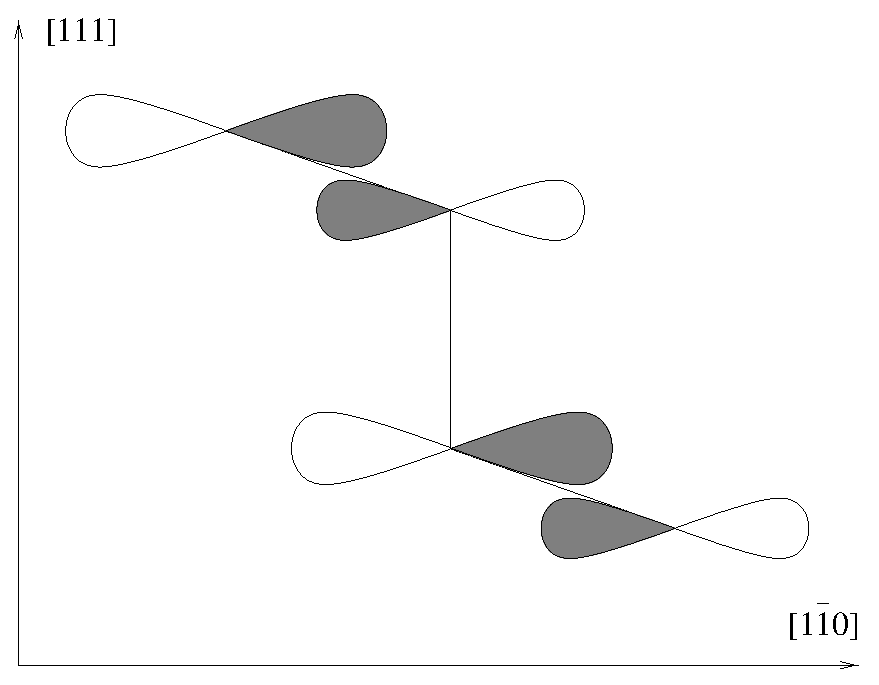
\includegraphics[width=10cm]{G5v.x.eps}\raisebox{4cm}{(b)}
  \caption{Schematische Darstellung der Wellenfunktionen von (a) \GCB\ und (b)
  \GVBx. $[1 \bar 1 0]$ entspricht der $x$-Richtung, $[111]$ der 
  $z$-Richtung. }
  \label{fig:wfkt-G}
\end{figure}
%\end{sidewaysfigure}

%\begin{sidewaysfigure}
\begin{figure}
  \centering
  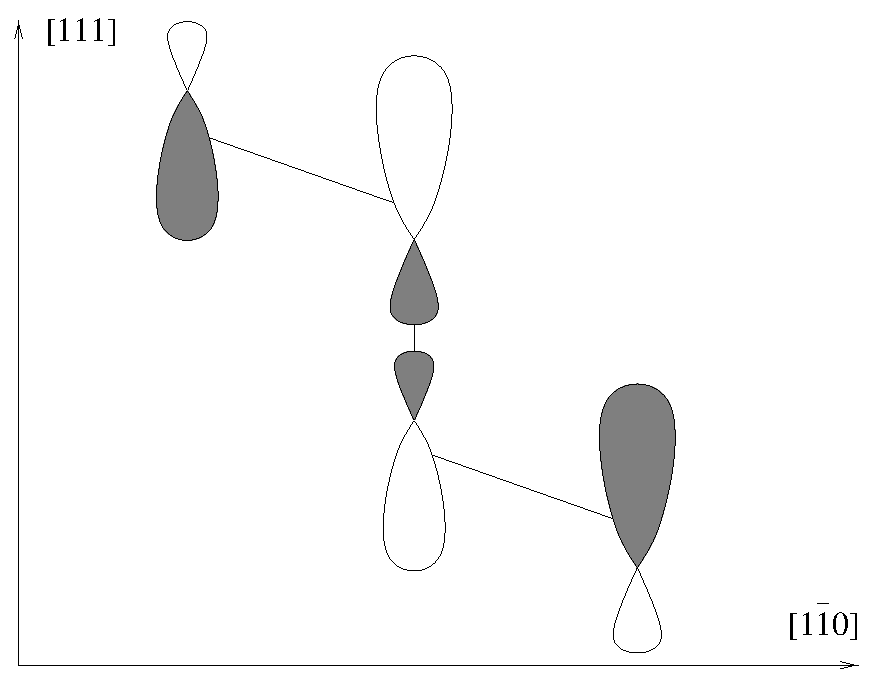
\includegraphics[width=10cm]{L1c.eps}\raisebox{4cm}{(a)}
  \vspace{2ex}
  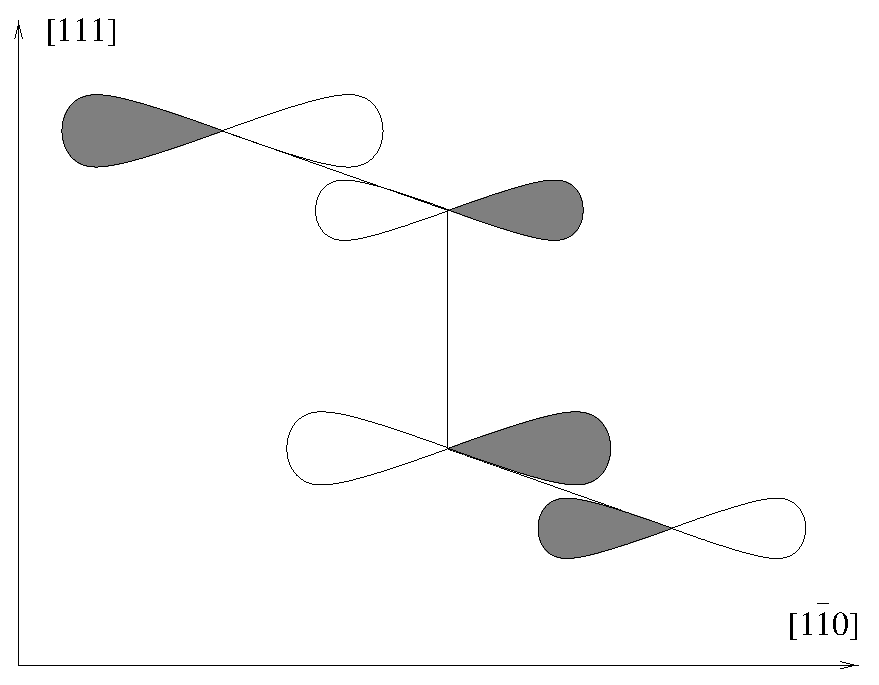
\includegraphics[width=10cm]{L3v.x.eps}\raisebox{4cm}{(b)}
  \caption{Schematische Darstellung der Wellenfunktionen von (a) \LCB\ und (b)
  \LVBx. $[1 \bar 1 0]$ entspricht der $x$-Richtung, $[111]$ der
  $z$-Richtung.}
  \label{fig:wfkt-L}
\end{figure}
%\end{sidewaysfigure}

Dadurch, da"s wir uns nun auf bestimmte Phasen der Wellenfunktionen in unserer
Basis festgelegt haben, sind im Prinzip auch die Vorzeichen der
Potentialmatrixelemente festgelegt. Doch treten dabei Schwierigkeiten auf, die
wir am Beispiel das Matrixelementes \V{35} illustrieren wollen. 

Die in Abb.~\ref{fig:wfkt-G}(b) und Abb.~\ref{fig:wfkt-L}(b) skizzierten
Valenzband-Wellenfunk"-ti"-onen lassen sich in der \CuPt-Einheitszelle als
%
\begin{subequations}
\label{eq:wfkt-tba}
\begin{eqnarray}
  \label{eq:G5v-tba}
  \ket{\GVBx} &=& -\alpha_{\Gamma} (\ket{x_{c1}} + \ket{x_{c2}})
  + \beta_{\Gamma} (\ket{x_{a1}} + \ket{x_{a2}}) \\
  \label{eq:L3v-tba}
  \ket{\LVBx} &=& +\alpha_{\text{L}} (\ket{x_{c1}} - \ket{x_{c2}}) +
  \beta_{\text{L}} (\ket{x_{a1}} - \ket{x_{a2}})
\end{eqnarray}
\end{subequations}
%
schreiben. Dabei sind $\alpha_{\Gamma}$, $\beta_{\Gamma}$, $\alpha_{\text{L}}$
und $\beta_{\text{L}}$ positive Konstanten. Die $\ket{x_{i}}$ sind auf dem
Atom $i$ [siehe Abb.~\ref{fig:wfkt-G}(a)] lokalisierte $p_{x}$-artige
Wellenfunktionen, deren positive H"alfte in positive $x$-Richtung
zeigt.\footnote{Genauer gesagt sind die $\ket{x_{i}}$ Blochsummen zu $k=0$
  "uber alle zu $i$ "aquivalente Atome im Kristall (siehe Anhang
  \ref{cha:lcao}).} 
Nun k"onnen wir den TBA-Hamilton-Operator, der den geordneten
Kristall beschreibt, in einen Teil \op{H_{0}^{\SSs \text{TBA}}}, der
Zinkblende Symmetrie besitzt, und einen Teil \op{H_{1}^{\SSs \text{TBA}}}, der
das Ordnungspotential beschreibt, aufteilen. Die Zust"ande in
Gl.~\eqref{eq:wfkt-tba} sind Eigenzust"ande von \op{H_{0}^{\SSs \text{TBA}}},
doch k"onnen wir das Matrixelement bez"uglich \op{H_{1}^{\SSs \text{TBA}}}
berechnen:
%
\begin{eqnarray}
  \label{eq:V35-tba}
  \matrixel{\GVBx}{\op{H_{1}^{\SSs \text{TBA}}}}{\LVBx} &=&
  - \alpha_{\Gamma} \alpha_{\text{L}} (\Delta E_{p}^{c1} - \Delta E_{p}^{c2})
  + \beta_{\Gamma}  \beta_{\text{L}}  (\Delta E_{p}^{a1} - \Delta E_{p}^{a2})
  \nonumber\\ && 
  - (\beta_{\text{L}}\alpha_{\Gamma} - \beta_{\Gamma} \alpha_{\text{L}}) 
    ( \Delta p_{c1}p_{a1}\pi - \Delta p_{c2}p_{a2}\pi )
  \nonumber\\ &&
  + (\beta_{\text{L}}\alpha_{\Gamma} + \beta_{\Gamma} \alpha_{\text{L}}) 
    (\frac{4}{3}(\Delta p_{c1}p_{a2}\sigma - \Delta p_{c2}p_{a1}\sigma)
  \nonumber\\ && \hspace{6.78em}
  +  \frac{5}{3}(\Delta p_{c1}p_{a2}\pi    - \Delta p_{c2}p_{a1}\pi   ) ) 
\end{eqnarray}
%
Dabei bedeutet z.~B.\ $\Delta E_{p}^{c1}$ die "Anderung in der Energie eines
$p$-Orbitals auf dem Kation C1, $\Delta p_{c1}p_{a1}\pi$ die "Anderung in der
Energie einer $pp\pi$-Bindung zwischen Kation C1 und Anion A1
etc.\footnote{Eine genauere Erkl"arung der Bedeutung dieser Parameter ist in
  Anhang~\ref{cha:lcao} zu finden.}  Um diesen Ausdruck auswerten zu k"onnen,
ben"otigen wir sowohl die Koeffizienten $\alpha_{\Gamma}$, $\beta_{\Gamma}$,
$\alpha_{\text{L}}$ und $\beta_{\text{L}}$ sowie die "Anderungen in den
Parametern der TBA. Erstere lassen sich leicht f"ur einen Satz Parameter
berechnen oder aber auch absch"atzen, da sie sich kaum zwischen verschiedenen
Kristallen mit Zinkblende-Gitter unterscheiden. Um die "Anderung in den
TBA-Parametern zu beschreiben, bieten sich die Unterschiede zwischen den
entsprechenden Parametern f"ur GaP und InP an. F"ur diese sind verschieden
Parametrisierungen durchgef"uhrt worden \cite{harr:80,chad:77,jsbb:98}, doch
sind diese Parameter abstandsabh"angig und beziehen sich auf die in GaP bzw.
InP zu findenden atomaren Abst"ande. Die atomaren Abst"ande in \GaInP\ 
entsprechen aber mehr denen in GaAs, das als Substrat w"ahrend des Wachstums
verwendet wird. Die Schwierigkeit dabei ist, da"s die Abstandsabh"angigkeit
der TBA-Parameter nicht gut bekannt ist. So werden in der Literatur sehr
verschiedene Abh"angigkeiten diskutiert \cite[p.~504ff]{jsbb:98, harr:80}.
Trotzdem k"onnen Ausdr"ucke vom Typ \eqref{eq:V35-tba} f"ur verschiedene
Parametrisierungen und Abstandsabh"angigkeiten ausgewertet werden. Doch neben
den zu erwartenden starken Unterschieden in den Betr"agen, erhalten wir auch
f"ur die Vorzeichen und die relativen Vorzeichen der Matrixelemente
verschiedene Ergebnisse, je nach dem, welche Parametrisierung wir verwenden.
Wir k"onnen aber nicht sagen, da"s eine dieser Parametrisierungen den anderen
vorzuziehen ist. Deshalb m"ussen wir folgern, da"s diese Methode nicht
geeignet ist, die relativen Vorzeichen der Potentialmatrixelemente zu
bestimmen, weshalb wir die verschiedenen M"oglichkeiten bei der Auswertung des
Hamilton-Operators \eqref{eq:k.p-H} ber"ucksichtigen m"ussen.


%%% Local Variables: 
%%% mode: latex
%%% TeX-master: "diplom"
%%% End: 



%%% Local Variables: 
%%% mode: latex
%%% TeX-master: "diplom"
%%% End: 






% Ergebnisse
%%% Kapitel �ber Diagonalisierung von H, Ergebnisse und Diskussion
%%% Time-stamp: <1999-03-04 13:59:35 ralf>

\chapter{Ergebnisse und Diskussion}
\label{cha:ergebnisse}

%%%%%%%%%%%%%%%%%%%%%%%%%%%%%%%%%%%%%%%%%%%%%%%%
\section{Diagonalisieren des Hamilton-Operators}
\label{sec:diag}

Die Diagonalisierung des \kdotp-Hamilton-Operators \eqref{eq:k.p-H} wollen wir
in mehreren Schritten vornehmen. Die Idee dabei ist, da"s wir zun"achst
Gl.~\eqref{eq:k.p-H} f"ur $k=0$ diagonalisieren. Dadurch erhalten wir neue
Basisfunktionen, die sich als Linearkombination der alten Basisfunktionen
darstellen lassen, so da"s wir die \kdotp-Wechselwirkungen zwischen diesen
neuen Basisfunktionen angeben k"onnen. Danach k"onnen wir dann diese
Kopplungen in zweiter Ordnung St"orungstheorie behandeln, um die effektiven
Massen zu erhalten.


%%%%%%%%%%%%%%%%%%%%%%%
\subsection{Entkopplung von Valenz- und Leitungsband}
\label{sec:V15}

In Gl.~\eqref{eq:V15-V11} haben wir gesehen, da"s \V{15}, verglichen mit
den dazugeh"origen Energienennern, das Matrixelement mit dem geringsten Effekt
ist. Wie wir noch sehen werden, gilt $|\V{11}| \approx 200$~meV f"ur die
h"ochstgeordneten Proben, die im Experiment bisher gefunden wurden. Setzen wir
aber nun die Werte aus Tab.~\ref{tab:Em*P} ein, so erhalten wir, da"s auch
$|\V{15}| \approx 200$~meV ist und damit eine Gr"o"senordnung kleiner als
der dazugeh"orige Energienenner. Dies rechtfertigt es, diese Kopplung
st"orungstheoretisch zu behandeln.

Dabei wollen wir L"owdin-St"orungstheorie \cite{lowd:51} verwenden, wie wir
sie in Kap.~\ref{sec:standard-k.p} beschrieben haben.  Da wir hier eine
Entkopplung von Valenz- und Leitungsband durchf"uhren m"ochten, bedeutet dies,
da"s wir einmal die Leitungsb"ander als Gruppe \raum{A} betrachten und die
Valenzb"ander als Gruppe \raum{B} und dann diese Rollen vertauschen.

F"uhren wir dies f"ur den Hamilton-Operator \eqref{eq:k.p-H} durch, so m"ussen
wir nur folgende Energien ab"andern, um die Kopplung zwischen Valenz- und
Leitungsband in zweiter Ordnung zu beseitigen:
%
%\begin{subequations}
%\label{eq:E-shift}
\begin{eqnarray*}
%  \label{eq:EL-shift}
  \tilde{E}_{\text{Lc}} &=& E_{\text{Lc}} + \frac{|\V{15}|^{2}}{E_{\text{Lc}}}\\
%  \label{eq:EG-shift} 
  \tilde{E}_{\Gamma \text{v}}^{z} &=& - \frac{|\V{15}|^{2}}{E_{\text{Lc}}}
\end{eqnarray*}
%\end{subequations}
%
Die schwache Beimischung von \LCB-Anteilen zum \GVBz-Zustand und umgekehrt
soll im folgenden vernachl"assigt werden. 

Der gro"se Vorteil bei diesem Zugang ist, da"s wir nur den Betrag von \V{15}
ben"otigen, nicht aber dessen Vorzeichen. Damit haben wir die Anzahl der
M"oglichkeiten, die wir diskutieren m"ussen, auf zwei reduziert. Entweder haben
\V{11} und \V{35} gleiches Vorzeichen, oder verschiedenes. Der Nachteil ist,
da"s die Aussagekraft unseres Modells f"ur sehr hohen Ordnungsgrad nachl"a"st. 



%%%%%%%%%%%%%%%%%%%%%%
\subsection{Zwei-Niveau-Systeme}
\label{sec:2niveau}

Der n"achste Schritt ist die Diagonalisierung bez"uglich \V{11} und \V{35},
die einfach ist, da es sich dabei im Leitungs- und Valenzband um zwei
Zwei-Niveau-Systeme  handelt.

Im Leitungsband erhalten wir dadurch die Zust"ande
%
\begin{subequations}
\label{eq:CB-V}
\begin{eqnarray}
  \label{eq:GCB-V}
  \ket{\bGCB (\GCB)} &=& \alpha_{\text{c}} \ket{\GCB} + \beta_{\text{c}}
  \ket{\LCB}  \\
  \label{eq:LCB-V}
  \ket{\bGCB (\LCB)} &=& \beta_{\text{c}} \ket{\GCB} - \alpha_{\text{c}}
  \ket{\LCB}
\end{eqnarray}
\end{subequations}
%
mit den Eigenenergien
%
\begin{equation}
  \label{eq:E-CB-V}
  E_{\text{c}}^{(1/2)} = \frac{E_{\Gamma \text{c}} + \tilde E_{\text{Lc}}}{2}
  \mp \sqrt{\left( \frac{E_{\Gamma \text{c}} - \tilde E_{\text{Lc}}}{2}
  \right)^{2} + |\V{11}|^{2} } .
\end{equation}
%
Au"serdem gilt
%
\begin{subequations}
\label{eq:koeffCB}
\begin{eqnarray}
  \label{eq:alphaCB}
  \alpha_{\text{c}} &=& \frac{\V{11}}{\sqrt{\left( E_{\Gamma \text{c}} -
        E_{\text{c}}^{(1)} \right)^{2} + |\V{11}|^{2} }} \\
  \label{eq:betaCB}
  \beta_{\text{c}} &=& \frac{E_{\text{c}}^{(1)} - E_{\Gamma \text{c}}}
  {\sqrt{\left( E_{\Gamma \text{c}} - E_{\text{c}}^{(1)} \right)^{2} +
      |\V{11}|^{2} }} .
\end{eqnarray}
\end{subequations}
%
Dabei ist $E_{\text{c}}^{(1)}$ die Eigenenergie zu \ket{\bGCB (\GCB)} und
bezieht sich auf das Minuszeichen in Gl.~\eqref{eq:E-CB-V}.

Im Valenzband erhalten wir\footnote{Hier f"ur \bGVBx, analoges gilt auch f"ur
  \bGVBy} 
%
\begin{subequations}
\label{eq:VB-V}
\begin{eqnarray}
  \label{eq:GVB-V}
  \ket{\bGVBx (\GVBx)} &=& \alpha_{\text{v}} \ket{\GVBx} + \beta_{\text{v}}
  \ket{\LVBx}  \\
  \label{eq:LVB-V}
  \ket{\bGVBx (\LVBx)} &=& \beta_{\text{v}} \ket{\GVBx} - \alpha_{\text{v}}
  \ket{\LVBx}
\end{eqnarray}
\end{subequations}
%
mit den Eigenenergien
%
\begin{equation}
  \label{eq:E-VB-V}
  E_{\text{v}}^{(1/2)} = \frac{E_{\text{Lv}}}{2} \pm 
  \sqrt{\left( \frac{E_{\text{Lv}}}{2} \right)^{2} + |\V{35}|^{2} } .
\end{equation}
%
Au"serdem gilt
%
\begin{subequations}
\label{eq:koeffVB}
\begin{eqnarray}
  \label{eq:alphaVB}
  \alpha_{\text{v}} &=& \frac{\V{35}}
  {\sqrt{ {E_{\text{v}}^{(1)}}^{2} + |\V{35}|^{2} }} \\
  \label{eq:betaVB}
  \beta_{\text{v}} &=& \frac{E_{\text{v}}^{(1)}}
  {\sqrt{ {E_{\text{v}}^{(1)}}^{2} + |\V{35}|^{2} }} .
\end{eqnarray}
\end{subequations}
%
Dabei ist $E_{\text{v}}^{(1)}$ die Eigenenergie zu \ket{\bGVBx (\GVBx)} und
bezieht sich auf das Pluszeichen in Gl.~\eqref{eq:E-VB-V}.


%%%%%%%%%%%%%%%%%%%%%%%%
\subsection{Der neue \kdotp-Hamilton-Operator}
\label{sec:neu-k.p-H}


%%%%%%%%%%%% Neuer gesamt k.p Hamilton-Operator
%\begin{floateqnum}
\begin{sidewaysfloateqnum}
\begin{equation}
\label{eq:neu-k.p-H}
\caption{\kdotp-Hamilton-Operator bez"uglich Basis, die Ordnungspotential diagonalisiert.}
\renewcommand{\arraystretch}{1.6}
\op{H_{\bar \Gamma}} = \left(
\begin{array}{c|cc|c||c|cc}
  \raisebox{2.0em}[0ex][0ex]{\ket{\bGCB  (\GCB)}} 
& \raisebox{2.0em}[0ex][0ex]{\ket{\bGVBx (\GVBx)}} 
& \raisebox{2.0em}[0ex][0ex]{\ket{\bGVBy (\GVBy)}} 
& \raisebox{2.0em}[0ex][0ex]{\ket{\bGVB{1} (\GVBz)}} 
& \raisebox{2.0em}[0ex][0ex]{\ket{\bGCB  (\LCB)}} 
& \raisebox{2.0em}[0ex][0ex]{\ket{\bGVBx (\LVBx)}} 
& \raisebox{2.0em}[0ex][0ex]{\ket{\bGVBy (\LVBy)}} \\[-4ex]
%%%%%%%%%%%
\begin{array}[c]{c} E_{\text{c}}^{(1)} + \frac{\hbar^{2}}{2m} k^{2}\\
  + {\beta_{\text{c}}}^{2} G k_{z}^{2}
  \end{array} 
& i P_{1} k_{x} 
& i P_{1} k_{y} 
& i \pri{P_{1}} k_{z} 
& 0 
& - i P_{2} k_{x} 
& - i P_{2} k_{y} \\
\hline
%%%%%%%%%%%
  -i P_{1} k_{x} 
& E_{\text{v}}^{(1)} + \frac{\hbar^{2}}{2m}k ^{2} 
& 0 
& 0 
& - i P_{2} k_{x} 
& 0 
& 0 \\
%%%%%%%%%%%
  -i P_{1} k_{y} 
& 0 
& E_{\text{v}}^{(1)} + \frac{\hbar^{2}}{2m} k^{2} 
& 0 
& - i P_{2} k_{y}
& 0 
& 0   \\
%%%%%%%%%%%
\hline
  -i \pri{P_{1}} k_{z} 
& 0 
& 0 
& \tilde E^{z}_{\Gamma \text{v}} + \frac{\hbar^{2}}{2m} k^{2} 
& - i \pri{P_{2}} k_{z}
& 0 
& 0 \\
\hline\hline
%%%%%%%%%%%
0 
& i P_{2} k_{x}
& i P_{2} k_{y}
& i \pri{P_{2}} k_{z}
& \begin{array}[c]{c} E_{\text{c}}^{(2)} + \frac{\hbar^{2}}{2m} k^{2}\\
  + {\alpha_{\text{c}}}^{2} G k_{z}^{2}
  \end{array} 
& i P_{1} k_{x} 
& i P_{1} k_{y}\\
%%%%%%%%%%%
\hline
i P_{2} k_{x} 
& 0 
& 0 
& 0 
& -i P_{1} k_{x} 
& E_{\text{v}}^{(2)} + \frac{\hbar^{2}}{2m} k^{2} 
& 0 \\
%%%%%%%%%%%
i P_{2} k_{y}
& 0 
& 0 
& 0 
& -i P_{1} k_{y} 
& 0 
& E_{\text{v}}^{(2)} + \frac{\hbar^{2}}{2m} k^{2} \\
\end{array} \right)
\renewcommand{\arraystretch}{0.625}
\end{equation}
%\end{floateqnum}
\end{sidewaysfloateqnum}
%%%%%%%%%%%%%%%%%%%%%%%%%%%%%%%

Verwenden wir nun die neuen Basisfunktionen Gln.~\eqref{eq:CB-V} und
\eqref{eq:VB-V}, die diagonal bez"uglich der Potentialmatrixelemente sind, und
betrachten die \kdotp-Matrix \eqref{eq:k.p-H} in dieser Basis, so erhalten wir
eine neue Matrix, die in Gl.~\eqref{eq:neu-k.p-H} (siehe
S.~\pageref{eq:neu-k.p-H}) angegeben ist. Dabei wurden folgende Abk"urzungen
verwendet:
%
\begin{subequations}
\label{eg:P1-P2'}
\begin{eqnarray}
  \label{eq:P1}
  P_{1} &=& (\alpha_{\text{v}} \alpha_{\text{c}} + \beta_{\text{v}}
  \beta_{\text{c}}) \PG \\
  \label{eq:P2}
  P_{2} &=& (\alpha_{\text{v}} \beta_{\text{c}} - \beta_{\text{v}}
  \alpha_{\text{c}}) \PG \\
  \label{eq:P1'}
  \pri{P_{1}} &=& \alpha_{\text{c}} \PG \\
  \label{eq:P2'}
  \pri{P_{2}} &=& \beta_{\text{c}} \PG
\end{eqnarray}
\end{subequations}
%
Daraus erhalten wir nun direkt die effektiven Massen in den untersten beiden
Leitungsb"andern, indem wir Gl.~\eqref{eq:neu-k.p-H} in zweiter Ordnung
St"orungstheorie bez"uglich $k$ diagonalisieren. 

F"ur den \bGCB (\GCB)-Zustand erhalten wir:
%
\begin{subequations}
\label{eq:m*-GCB-G}
\begin{eqnarray}
  \label{eq:m*-GCB-G.parallel}
  \frac{m}{m_{\parallel}^{(1)}} &=& 1 + \frac{2m}{\hbar^{2}} \left(
    \beta_{\text{c}}^{2} G + \frac{|\pri{P_{1}}|^{2}}{E_{\text{c}}^{(1)} -
      \tilde E^{z}_{\Gamma \text{v}}} \right) \\
  \label{eq:m*-GCB-G.senkrecht}
  \frac{m}{m_{\perp}^{(1)}} &=& 1 + \frac{2m}{\hbar^{2}} \left(
    \frac{|P_{1}|^{2}}{E_{\text{c}}^{(1)} - E^{(1)}_{\text{v}}} +
    \frac{|P_{2}|^{2}}{E_{\text{c}}^{(1)} - E^{(2)}_{\text{v}}} \right)
\end{eqnarray}
\end{subequations}
%
Dabei gilt $m_{\parallel}^{(1)}$ f"ur die Richtung parallel zur
Ordnungsrichtung, d.~h.\ der $[111]$-Richtung , $m_{\perp}^{(1)}$ senkrecht zu
dieser.  

F"ur das \bGCB (\LCB)-Niveau ergibt sich
%
\begin{subequations}
\label{eq:m*-GCB-L}
\begin{eqnarray}
  \label{eq:m*-GCB-L.parallel}
  \frac{m}{m_{\parallel}^{(2)}} &=& 1 + \frac{2m}{\hbar^{2}} \left(
    \alpha_{\text{c}}^{2} G + \frac{|\pri{P_{2}}|^{2}}{E_{\text{c}}^{(2)} -
      \tilde E^{z}_{\Gamma \text{v}}} \right) \\
  \label{eq:m*-GCB-L.senkrecht}
  \frac{m}{m_{\perp}^{(2)}} &=& 1 + \frac{2m}{\hbar^{2}} \left(
    \frac{|P_{1}|^{2}}{E_{\text{c}}^{(2)} - E^{(2)}_{\text{v}}} +
    \frac{|P_{2}|^{2}}{E_{\text{c}}^{(2)} - E^{(1)}_{\text{v}}} \right)
\end{eqnarray}
\end{subequations}
%
mit entsprechenden Bedeutungen von $m_{\parallel}^{(2)}$ und $m_{\perp}^{(2)}$.

An dieser Stelle sehen wir auch, wie die in Kap.~\ref{sec:phase} diskutierten
Phasen der Matrixelemente eingehen. Denn zum einen h"angen $\alpha_{\text{c}}$
und $\alpha_{\text{v}}$ direkt vom Vorzeichen der Potentialmatrixelemente
\V{11} bzw.\ \V{35} ab. Zum anderen geht auch ein, da"s $\PG = \PL$ gilt. Es
f"allt allerdings auf, da"s die beiden Massen parallel zur Ordnungsrichtung
$m^{(1/2)}_{\parallel}$ nicht von den Phasenbeziehungen abh"angen, da hier von
phasenabh"angigen Gr"o"sen nur Betragsquadrate eingehen.


%%%%%%%%%%%%%%%%%%%%%%%%%%%%%%%%%%%%%%%
\section{Ergebnisse}
\label{sec:ergeb}

Die im vorhergehenden Abschnitt abgeleiteten Formeln lassen sich f"ur
verschiedene Werte von \V{11} numerisch l"osen. Da \V{11} der einzige freie
Parameter in unserem Modell ist, werden wir die Ergebnisse solch einer
Rechnung auch in Abh"angigkeit von \V{11} darstellen. Experimentell ist es
aber kaum m"oglich, 
\V{11} zu bestimmen, weshalb wir in Anhang~\ref{cha:ergeb-BGR} diese Ergebnisse
auch als Funktion der Bandl"uckenreduzierung zeigen.

%%%%%%%%%%%%%%
\subsection{Energieeigenwerte}
\label{sec:energie}

Zun"achst wollen wir die Bandkantenenergien betrachten, wie sie sich aus
unserer Rechnung ergeben. Abb.~\ref{fig:energie}(a) zeigt, wie sich
Bandl"uckenreduzierung $\Delta E_{\text{BGR}}$, Kristallfeldaufspaltung
$\Delta_{\text{CF}}$ und "Anderung $\Delta E_{\Gamma \rightarrow \text{L}}$ der
"Ubergangsenergie $\bGVB{3}(\GVB) \rightarrow \bGCB (\LCB)$ als Funktion von
\V{11} verhalten. Dabei wird \V{11} als positiv angenommen, da die hier
diskutierten Ph"anomene nicht von den absoluten Phasen der Matrixelemente
abh"angen. Das liegt unter anderen daran, da"s ein Austausch von Ga- und
In-reichen Lagen an der Physik der geordneten Struktur nichts "andern kann,
aber zu einem Vorzeichenwechsel bei den Matrixelementen f"uhrt.

\begin{figure}[htb]
  \centering 
  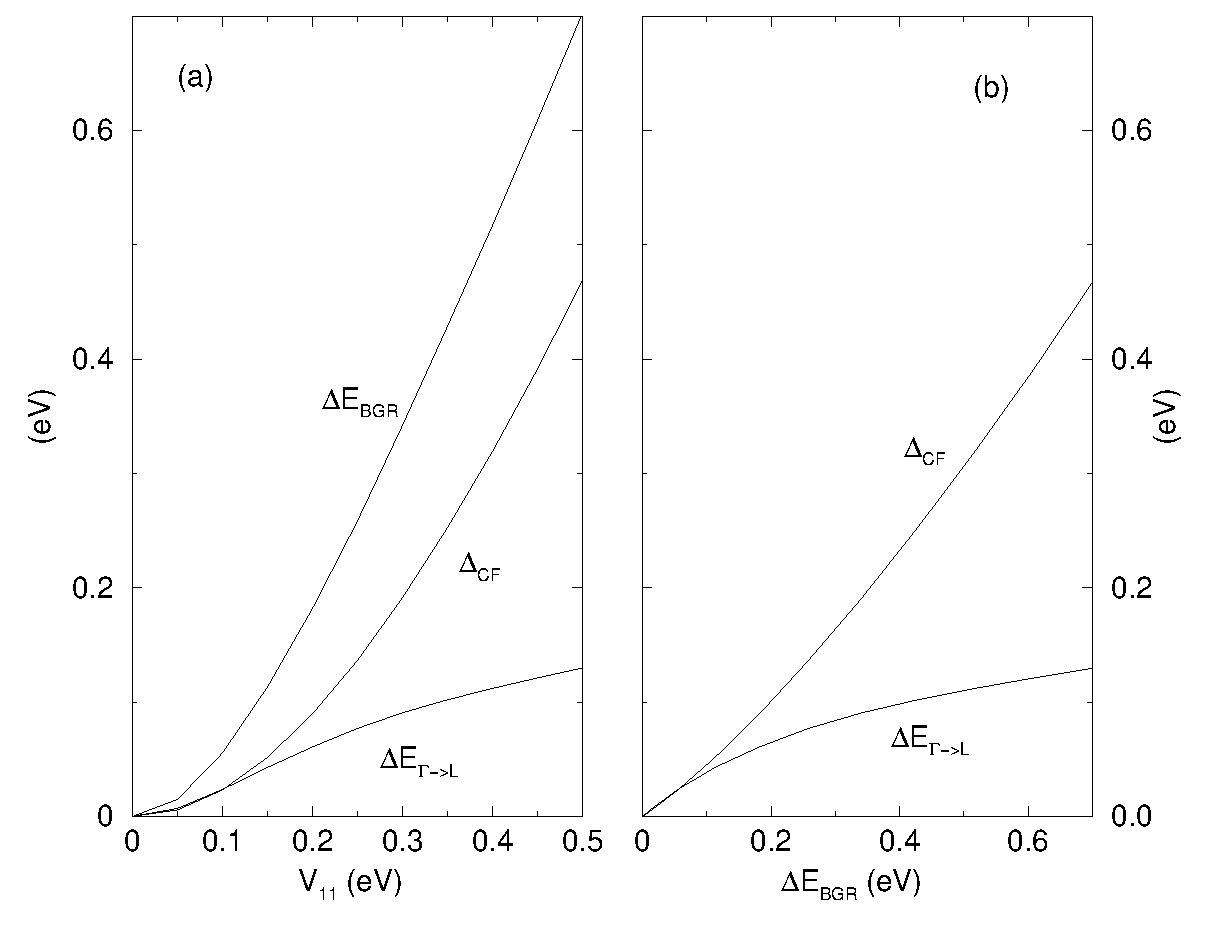
\includegraphics[width=\textwidth]{BGR.CF.eps}
  \caption{(a) Bandl"uckenreduzierung $\Delta E_{\text{BGR}}$,
  Kristallfeldaufspaltung $\Delta_{\text{CF}}$ und "Anderung $\Delta E_{\Gamma
  \rightarrow \text{L}}$ der "Ubergangsenergie $\bGVB{3}(\GVB) \rightarrow
  \bGCB (\LCB)$ als Funktion von \V{11}. (b) Kristallfeldaufspaltung
  $\Delta_{\text{CF}}$ und "Anderung $\Delta E_{\Gamma \rightarrow \text{L}}$
  der "Ubergangsenergie $\bGVB{3}(\GVB) \rightarrow \bGCB (\LCB)$ als Funktion
  der Bandl"uckenreduzierung $\Delta E_{\text{BGR}}$.}
  \label{fig:energie}
\end{figure}

Die Betrachtung der Bandkantenergien ist notwendig, weil wir sonst nicht
wissen k"onnen, wie gro"s unsere Matrixelemente sein m"ussen, um einen
Kristall mit einem bestimmten Ordnungsgrad zu beschreiben.

An den h"ochstgeordneten Proben, die heute hergestellt werden k"onnen, werden
typischerweise Bandl"uckenreduzierungen von $100 \dots 150$~meV gemessen
\cite{ezdm:97,kipp:97}. Solche Werte erhalten wir f"ur $\V{11} = 150 \dots
200$~meV. $\V{11} = 0 \dots 200$~meV ist also der Bereich, der realistische
Proben beschreibt. Wie bereits in Kap.~\ref{sec:V15} erw"ahnt,
ist dies auch der Bereich, in dem die St"orungstheorie f"ur \V{15}
gerechtfertigt ist. Vorhersagen f"ur im Experiment beobachtete Proben
sind also m"oglich. Bei Aussagen "uber st"arker geordnete Proben ist
zudem zu beachten, da"s Gln.~\eqref{eq:zeta} und \eqref{eq:theta} nicht
mehr erf"ullt sein m"ussen, was die Verh"altnisse zwischen den
Potentialmatrixelementen ver"andern w"urde.

Wei und Zunger \cite{wezu:98} geben 430~meV als theoretische
Bandl"uckenabsenkung der ideal geordneten Struktur an. Wie aus
Abb.~\ref{fig:energie} ersichtlich, erhalten wir diesen Wert f"ur $\V{11}
\approx 350$~meV. Wir werden uns deshalb bei weiteren Darstellungen auf den
Bereich zwischen 0~meV und 350~meV f"ur \V{11} beschr"anken. Diese
Abbildungen, die Impulsmatrixelemente und effektive Massen als Funktion von
\V{11} zeigen, werden so aufgebaut sein, da"s auf der linken Seite der Fall
gleichen Vorzeichens von \V{11} und \V{35} zu sehen ist ("`Phase: +1"'), auf
der rechten Seite der Fall verschiedenen Vorzeichens ("`Phase: -1"').

Wie bereits in Kap.~\ref{sec:betrag} erw"ahnt, gilt $\V{11} \propto \eta$,
wenn das Ordnungspotential mit Hilfe der VCA modelliert wird. Laks, Wei und
Zunger \cite{lwz:92} trafen die allgemeine Vorhersage, da"s physikalische
Eigenschaften langreichweitig geordneter Systeme in Abh"angigkeit von
Ordnungsgrad $\eta$ im wesentlichen wie $\eta^{2}$ skalieren. Wenn also
$\V{11} \propto \eta$ gilt, so l"a"st dies eine $\V{11}^{\; 2}$-Abh"angigkeit
erwarten. F"ur $\Delta E_{\text{BGR}}$ und $\Delta_{\text{CF}}$ ist dies auch
gut erf"ullt, wie Abb.~\ref{fig:energie}(a) und der nahezu lineare
Zusammenhang zwischen diesen Gr"o"sen in Abb.~\ref{fig:energie}(b) zeigt. Doch
f"ur $\Delta E_{\Gamma \rightarrow \text{L}}$ ist dies nur f"ur kleine \V{11}
erf"ullt. Da"s dies f"ur kleine \V{11} gilt, ist leicht "uber die 2. Ordnung
einer St"orungstheorie f"ur kleines \V{11} zu verstehen. Die f"ur gr"o"sere
Matrixelemente auftretenden Fehler scheinen sich f"ur $\Delta E_{\text{BGR}}$
und $\Delta_{\text{CF}}$ nahezu zu kompensieren, w"ahrend sie sich f"ur
$\Delta E_{\Gamma \rightarrow \text{L}}$ verst"arken.
 

%%%%%%%%%%%%%%
\subsection{Impulsmatrixelemente}
\label{sec:impulsme}

In Abb.~\ref{fig:P-me} sind die Impulsmatrixelemente, die in
Gl.~\eqref{eq:neu-k.p-H} auftreten, als Funktion von \V{11} zu sehen. Es f"allt
auf, da"s die Kurven f"ur $|\pri{P_{1}}|^{2}$ und $|\pri{P_{2}}|^{2}$
unabh"angig vom relativen Vorzeichen von \V{11} und \V{35} sind. Dies
l"a"st sich leicht verstehen, da in Gln.~\eqref{eq:P1'} und \eqref{eq:P2'}
keine Summen von Entwicklungskoeffizienten aus den Zwei-Niveau-Systemen
auftreten. Denn diese Summen, wie sie in Gln.~\eqref{eq:P1} und \eqref{eq:P2}
auftreten, f"uhren zu konstruktiver oder destruktiver "Uberlagerung der
\kdotp-Wechselwirkung zwischen $\Gamma$-Punkts-Wellenfunktionen einerseits und
L-Punkts-Wellenfunktionen andererseits. Haben z.~B.\ \V{11} und \V{35} das
gleiche Vorzeichen, so gilt dies auch f"ur $\alpha_{\text{c}}$ und
$\alpha_{\text{v}}$ [Gln.~\eqref{eq:alphaCB} und \eqref{eq:alphaVB}]. Dagegen
haben $\beta_{\text{c}}$ und $\beta_{\text{v}}$ immer verschiedenes Vorzeichen
[Gln. \eqref{eq:betaCB} und \eqref{eq:betaVB}]. Damit ergibt sich aus
Gl.~\eqref{eq:P1} ein stark abnehmendes $P_{1}$, wie es auch in
Abb.~\ref{fig:P-me} f"ur den Fall positiver relativer Phase zu sehen
ist.%\marginpar{St"orungstheorie...?}

\begin{figure}[htb]
  \centering 
  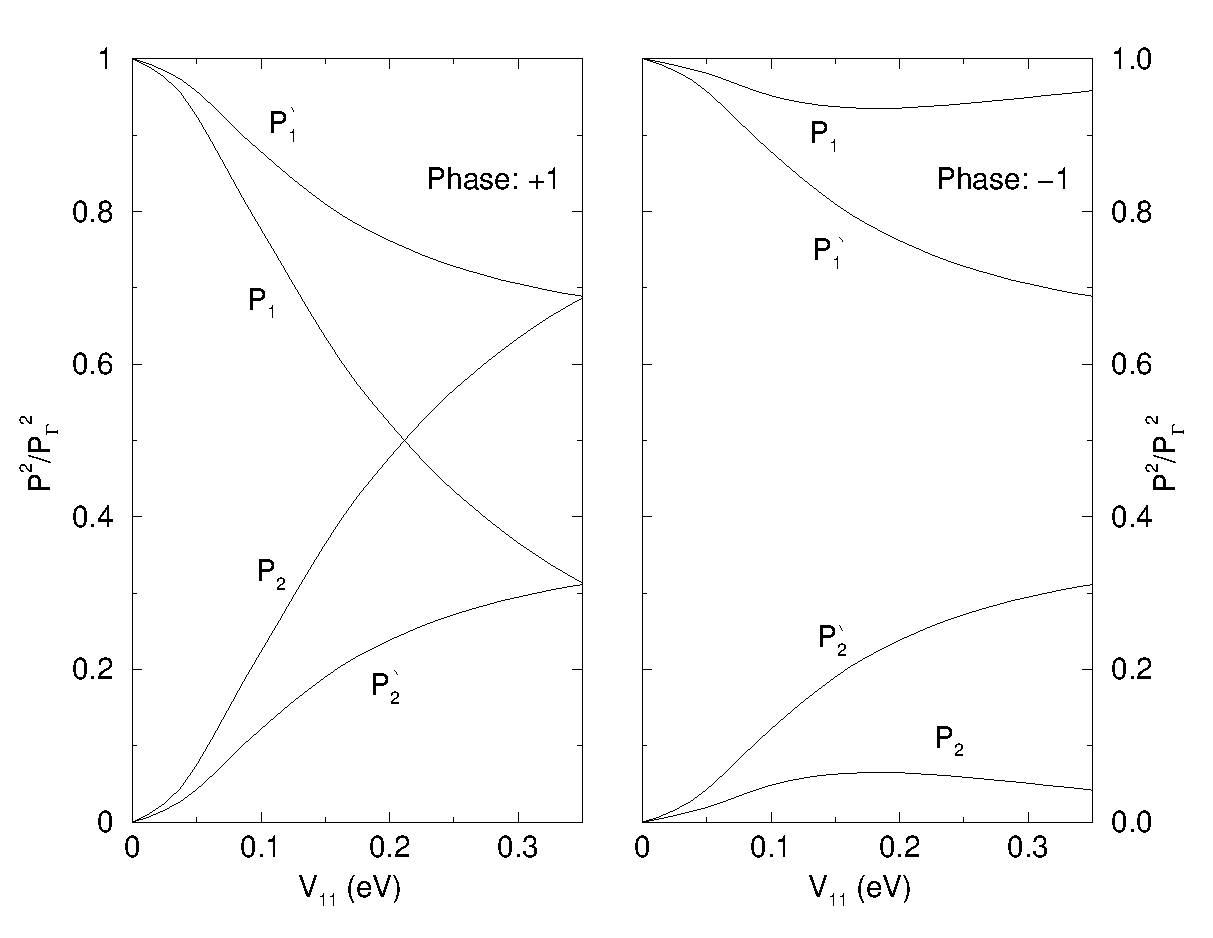
\includegraphics[width=\textwidth]{P2.eps}
  \caption{Betragsquadrat der Impulsmatrixelemente aus Gl.~\eqref{eq:neu-k.p-H}
  f"ur positives und negatives relatives Vorzeichen von \V{11} und \V{35} in
  Einheiten von $|\PG|^{2}$.} 
  \label{fig:P-me}
\end{figure}

Dabei spielen die Impulsmatrixelemente nicht nur f"ur die Bandkr"ummungen eine
entscheidende Rolle. Sie sind auch f"ur die St"arke optischer Dipol"uberg"ange
verantwortlich \cite{kitt:67}. So ist die Wahrscheinlichkeit eines "Ubergangs
$\bGVB{3} (\GVB) \rightarrow \bGCB (\GCB)$ proportional zu $|P_{1}|^{2}$, wenn
das Licht senkrecht zur Ordnungsrichtung polarisiert ist. F"ur die gleiche
Polarisationsrichtung beschreibt $|P_{2}|^{2}$ die Intensit"at des "Ubergangs
$\bGVB{3} (\GVB) \rightarrow \bGCB (\LCB)$. Dies erm"oglicht es, die relative
Phase von \V{11} und \V{35} zu bestimmen. Denn f"ur hochgeordnete Proben --
$\V{11} \approx 200$~meV -- sagt unsere Rechnung in etwa gleiche Intensit"at
f"ur diese "Uberg"ange voraus, wenn das relative Vorzeichen positiv ist. Ist
es negativ, so ist der "Ubergang $\bGVB{3} (\GVB) \rightarrow \bGCB (\LCB)$ um
etwa eine Gr"o"senordnung unterdr"uckt, wie aus Abb.~\ref{fig:P-me}
ersichtlich ist. Der letztere Fall beschreibt die im Experiment gefundenen
St"arken der Dipol"uberg"ange deutlich besser \cite{kksk:99}, so da"s wir mit
hoher Wahrscheinlichkeit davon ausgehen k"onnen, da"s das relative Vorzeichen
von \V{11} und \V{35} negativ ist. Da diese Bestimmung aber nicht vollst"andig
eindeutig ist, wollen wir trotzdem auch die Ergebnisse f"ur eine positive
relative Phase zeigen.

Wichtig sind diese Ergebnisse f"ur die Berechnung der
polarisations"-ab"-h"angigen Absorption \CuPt-geordneter \GaInP-Proben. In
bisherigen Rechnungen \cite{wezu:94-2,wezu:94} wurde immer von \emph{einem}
Dipolmatrixelement zwischen Zu"-st"an"-den im obersten Valenzband und im
untersten Leitungsband  ausgegangen. Dies gilt exakt aber nur im Grenzfall
verschwindender Ordnung, d.~h.\ kubischer Symmetrie. Denn vom Standpunkt der
Gruppentheorie aus betrachtet, gibt es keinen Grund warum
%
\begin{displaymath}
  \Matrixel{\bGCB (\GCB)}{\op{p_{z}}}{\bGVB{1} (\GVBz)} \stackrel{?}{=} 
  \Matrixel{\bGCB (\GCB)}{\op{p_{x}}}{\bGVB{3} (\GVBx)}
\end{displaymath}
%
gelten sollte, da \bGVB{1} (\GVBz) und \bGVB{3} (\GVBx) zu verschiedenen
Darstellungen der \Cdv\ geh"oren, und auch \op{p_{z}} und \op{p_{x}} sich
verschieden transformieren. Die in Abb.~\ref{fig:P-me} zu sehenden Ergebnisse
zeigen nun, da"s diese Ungleichheit nicht nur gilt, sondern da"s sie bereits
f"ur realistischen Ordnungsgrad nicht zu vernachl"assigen ist. Bei der
Auswertung polarisationsabh"angiger Messungen an "Uberg"angen vom
Va"-lenz"-band-Maximum zum \bGCB (\LCB) Zustand ist die Ber"ucksichtigung
dieser Ungleichheit besonders wichtig. Denn das Va"-lenz"-band-Maximum
enth"alt auf Grund der Spin-Bahn-Wechselwirkung sowohl \bGVB{3} als auch
\bGVB{1} Zust"ande, und die relativen Unterschiede zwischen $|P_{2}|^{2}$ und
$|\pri{P_{2}}|^{2}$ sind weit gr"o"ser als zwischen $|P_{1}|^{2}$ und
$|\pri{P_{1}}|^{2}$.

Das in Abb.~\ref{fig:P-me} f"ur eine positive Phase zu sehende Verhalten von
$|P_{1}|^{2}$ und $|\pri{P_{2}}|^{2}$ bzw.\ $|P_{2}|^{2}$ und
$|\pri{P_{1}}|^{2}$ k"onnte nahelegen, da"s sie sich einem gemeinsammen
Grenzwert ann"ahern. Tats"achlich schneiden sie sich nur und laufen danach
wieder auseinander. Da"s dieser Schnittpunkt so nahe an der oberen Grenze des
f"ur uns interessanten Bereichs liegt, erscheint zuf"allig zu sein.



%%%%%%%%%%%%%%
\subsection{Effektive Massen von \bGCB (\GCB)}
\label{sec:m*-GCB}

In Abb.~\ref{fig:m*-GCB} sind nun die Vorhersagen unseres Modells f"ur die
Ordnungsabh"angigkeit der effektiven Masse des \bGCB (\GCB)-Niveaus, d.~h.\
des untersten Leitungsbandes, zu sehen, wie sie sich aus
Gln.~\eqref{eq:m*-GCB-G} ergeben. 

\begin{figure}[htb]
  \centering
  \includegraphics[width=\textwidth]{masses.G.eps}
  \caption{Effektive Massen von \bGCB (\GCB) f"ur positives und negatives
    relatives Vorzeichen von \V{11} und \V{35}.} 
  \label{fig:m*-GCB}
\end{figure}

"Ahnlich wie in Abb.~\ref{fig:P-me} f"allt auf, da"s eine der Gr"o"sen -- hier
die effektive Masse parallel zur Ordnungsrichtung $m_{\parallel}$ --
unabh"angig vom relativen Vorzeichen der Potentialmatrixelemente ist. Dies
k"onnen wir wiederum darauf zur"uckf"uhren, da"s in
Gl.~\eqref{eq:m*-GCB-G.parallel} keine Summen von Entwicklungskoeffizienten
aus den Zwei-Niveau-Systemen auftreten. F"ur den Anstieg in $m_{\parallel}$
ist die Mischung von \GCB- mit \LCB-Zust"anden verantwortlich, da sie
$|\pri{P_{1}}|$ gegen"uber \PG\ verkleinert und die sehr flache Dispersion des
\LCB-Niveaus in $[111]$-Richtung beigemischt wird.

Dagegen verh"alt sich $m_{\perp}$ sehr unterschiedlich, wenn sich die relative
Phase von \V{11} zu \V{35} "andert. Dies k"onnen wir leicht durch das
unterschiedliche Verhalten von $|P_{1}|^{2}$ und $|P_{2}|^{2}$
verstehen. Unabh"angig von der relativen Phase verkleinern sich die
Energienenner in Gl.~\eqref{eq:m*-GCB-G.senkrecht}. Doch im Falle positiver
Phase beobachten wir einen starken Abfall in $|P_{1}|^{2}$ (siehe
Abb.~\ref{fig:P-me}), der sich nicht durch den Anstieg in $|P_{2}|^{2}$
kompensieren l"a"st, da das \bGVB{3} (\LVB)-Niveau etwa 1~eV tiefer als das
\bGVB{3} (\GVB)-Niveau liegt. F"ur negative Phase "andern sich die
Impulsmatrixelemente viel weniger, so da"s die Bandl"uckenreduzierung hier
voll zutragen kommt und eine stark ausgepr"agt Anisotropie der effektiven
Masse von $(m_{\parallel} - m_{\perp})/m_{\Gamma}^{\text{c}} = 0,489$ f"ur
$\V{11} = 350$~meV bzw. 0,217 f"ur $\V{11} = 150$~meV zu beobachten ist.

Wie wir im letzten Abschnitt erkl"art haben, beschreibt eine negative relative
Phase die beobachtete Absorption deutlich besser, als eine positive Phase, so
da"s die effektiven Massen f"ur negative Phase als unsere Vorhersage f"ur
teilgeordnetes \GaInP\ anzusehen sind. Vergleichen wir diese Ergebnisse mit
Dichtefunktionaltheorie Rechnungen von Franceschetti \emph{et al.}
\cite{fwz:95}, so stellen wir eine qualitative und teilweise auch quantitative
"Ubereinstimmung fest. So finden sie eine Anisotropie von 0,46 f"ur
vollst"andig geordnetes \GaInP, sehr nahe an unserem Wert von 0,489. Das
qualitative Bild einer Erh"ohung der effektiven Masse in Ordnungsrichtung und
einer Erniedrigung senkrecht dazu ist ebenfalls identisch. Nur die
Verh"altnisse verschieben sich etwas. Sie stellen nur eine sehr geringe
Reduktion der effektiven Masse senkrecht zur Ordnungsrichtung fest, w"ahrend
der Anstieg parallel zur Ordnungsrichtung ausgepr"agter ausf"allt. Dieser
Unterschied k"onnte auf die Methode, die bei der Korrektur des LDA-Fehlers
angewendet wurde, zur"uckzuf"uhren sein.

Das bisher einzige Experiment, das die Anisotropie der effektiven
Masse im untersten Leitungsband untersucht, wurde von Ernst \emph{et al.}
\cite{ezdm:97} durchgef"uhrt. Sie bestimmten die effektive Exzitonen-Masse
f"ur verschieden stark geordnete Proben mit Hilfe von
Photolumineszenz-Messungen im Magnetfeld. Auch sie fanden einen Anstieg
parallel zur 
Ordnungsrichtung und ein Absinken der effektiven Exzitonen-Masse senkrecht zu
ihr, stimmen also qualitativ mit den theoretische Vorhersagen "uberein. Ein
quantitativer Vergleich ist allerdings schwierig, da "uber die  "Anderungen in
den effektiven Massen der Valenzb"ander wenig bekannt ist.
 

%%%%%%%%%%%%%%
\subsection{Effektive Massen von \bGCB (\LCB)}
\label{sec:m*-LCB}

Die effektiven Massen, die sich aus Gln.~\eqref{eq:m*-GCB-L} ergeben, sind in
Abb.~\ref{fig:m*-LCB} dargestellt.  Auch hier ist die effektiven Masse
parallel zur Ordnungsrichtung $m_{\parallel}$ unabh"angig von der relativen
Phase der Potentialmatrixelemente. Die Erkl"arung f"ur dieses Verhalten ist
analog zu der im letzten Abschnitt pr"asentierten, nur die Rollen von $P_{1}$
und $P_{2}$ m"ussen vertauscht werden.  Der auff"alligsten Effekt, den wir
beobachten k"onnen, ist der starke Abfall in $m_{\parallel}$ von $1,7 m$ auf
unter $0,4 m$. Dies ist auf die Beimischung des \GCB-Zustandes
zur"uckzuf"uhren. Denn auf Grund dieser Beimischung besteht nun eine
\mbox{\kdotp}-Kopplung f"ur \vec{k} parallel zur Ordnungsrichtung zwischen dem
\bGCB (\LCB)-Zu"-stand und dem Valenzbandmaximum. Zuvor wurde $m_{\parallel}$
nur durch den Fernbandbeitrag $G$ bestimmt.

\afterpage{\clearpage
\begin{figure}[H]%[htb]
  \centering
  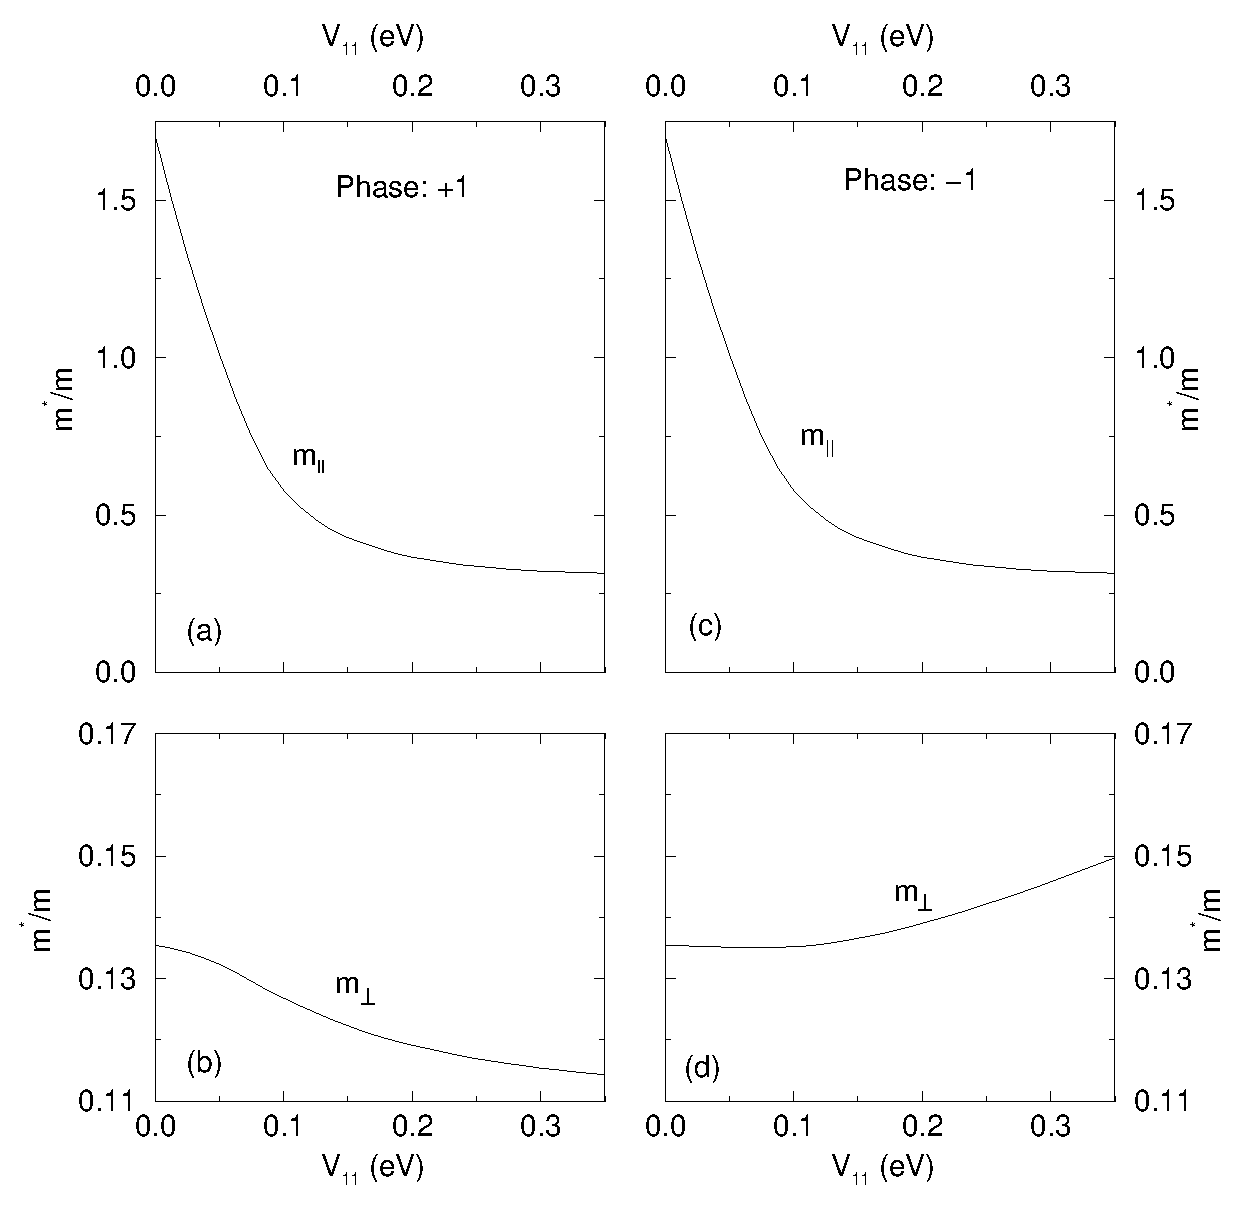
\includegraphics[width=\textwidth]{masses.L2.eps}
  \caption{Effektive Massen von \bGCB (\LCB) f"ur (a) und (b) positives sowie
  (c) und (d) negatives relatives Vorzeichen von \V{11} und \V{35}.} 
  \label{fig:m*-LCB}
\end{figure}
}


Die "Anderungen der effektiven Masse senkrecht zur Ordnungsrichtung
$m_{\perp}$ sind dagegen von "ahnlicher Gr"o"se wie die f"ur den \bGCB
(\GCB)-Zustand, nur da"s sich die Vorzeichen der "Anderungen vertauschen. Auch
dies l"a"st sich leicht verstehen, wenn wir den funktionalen Zusammenhang
zwischen den effektiven Massen und den Impulsmatrixelementen
\eqref{eq:m*-GCB-L} betrachten und das Verhalten der Impulsmatrixelemente aus
Abb.~\ref{fig:P-me} ber"ucksichtigen.

Wir k"onnen diese Vorhersagen nicht mit experimentellen oder anderen
theoretischen Ergebnissen vergleichen, da  noch niemand
dies gemessen hat, und es bei theoretischen Untersuchungen bisher nicht
ver"offentlicht wurde. Diese Abh"angigkeiten zu messen ist wahrscheinlich
nicht einfach, doch w"urde dies verdeutlichen wie wichtig eine korrekte
Beschreibung der $\Gamma$--L-Mischung f"ur \CuPt-geordnete Materialien ist.
Eine st"orungstheoretische Beschreibung dieser Wechselwirkung, wie sie noch in
Ref.~\cite{zhma:95} vorgeschlagen wurde, erscheint nicht m"oglich.
 
%%%%%%%%%%%%%%%%%%%%%%%%%%%%%%%%%%%%%%%%%%%%%
\section{Erweiterungen und Verbesserungen des Modells}
\label{sec:mehr+besser}

In Kap.~\ref{sec:ergeb} haben wir gezeigt, da"s unser Modell in guter
"Ubereinstimmung mit bisherigen Resultaten bez"uglich der Dispersion des
untersten Leitungsbandes steht, viele der beobachteten Effekte auch erkl"aren
kann und neue Vorhersagen liefert. Es gibt aber noch M"oglichkeiten, wie
entweder die Genauigkeit der Vorhersagen verbessert werden kann, oder aber
Vorhersagen "uber andere Materialaspekte getroffen werden k"onnen. Diese
wollen wir nun kurz skizzieren.

Die G"ultigkeit unseres Modells f"ur den Fall sehr hoher Ordnung ist durch
unsere Behandlung der ordnungsbedingten Wechselwirkung zwischen Valenz- und
Leitungsband begrenzt. Um diese zu verbessern, haben wir die M"oglichkeit,
auch bez"uglich \V{15} exakt zu diagonalisieren oder in der St"orungsreihe
Terme h"oherer Ordnung sowie Mischung von Valenz- und Leitungsband-Zust"anden
zu ber"ucksichtigen. Das Hauptproblem w"aren dabei die unbekannten relativen
Vorzeichen der Matrixelemente.

Auch die Bestimmung der Betr"age der Potentialmatrixelemente lie"se sich noch
verbessern. In Kap.~\ref{sec:betrag} haben wir das Verh"altnis der Betr"age
aus einer Rechnung in zweiter Ordnung St"orungstheorie und dem Vergleich mit
verschiedenen experimentellen und theoretischen Untersuchungen erhalten. Diese
werden aber meist nicht f"ur den Fall geringer Ordnung durchgef"uhrt, wo
unsere St"orungstheorie gilt. Die meisten Messungen werden im Bereich
mittlerer Ordnung mit einer Bandl"uckenreduzierung von $40 \dots 140$~meV
durchgef"uhrt. All-Elektronen-Rechnungen gelten meist nur f"ur vollst"andig
geordnete Systeme.  Dies zeigt sich z.~B.\ in Abb.~\ref{fig:energie}(b). Die
Kristallfeldaufspaltung $\Delta_{\text{CF}}$ verl"auft f"ur kleine
Bandl"uckenreduzierungen $\Delta E_{\text{BGR}}$ flach, so wie wir es auch
angepa"st haben. Doch hat sie "uber den Gesamtbereich gesehen, eine etwas zu
gro"se Steigung. "Ahnliches ist auch bei der "Anderung $\Delta E_{\Gamma
  \rightarrow \text{L}}$ der "Ubergangsenergie $\bGVB{3}(\GVB) \rightarrow
\bGCB (\LCB)$ zu beobachten, nur da"s hier der Gesamtverlauf zu flach ist.
Eine M"oglichkeit w"are, an Stelle von Gln.~\eqref{eq:zeta} und
\eqref{eq:theta} entsprechend angepa"ste Werte f"ur den Fall geringer Ordnung
zu benutzen. Dann k"onnte eine verbesserte "Ubereinstimmung zwischen den
Energieeigenwerten in unserem Modell und denen anderer Untersuchungen auch
f"ur gr"o"seren Ordnungsgrad erreicht werden.

Eine m"ogliche Erweiterung des Modells ist die Beschreibung der
Energiedispersion im Valenzband sowie deren "Anderung auf Grund der
ordnungsinduzierten Wechselwirkungen. Dazu mu"s das Modell zun"achst in der
Lage sein, die Valenzband-Dispersion f"ur den Fall verschwindender Ordnung zu
beschreiben. Dies ist, wie wir in Kap.~\ref{sec:k.p-H} erw"ahnt haben,
innerhalb der gew"ahlten Basis nur unter Ber"ucksichtigung von entsprechenden
Fernbandbeitr"agen m"oglich. Doch ist es einfach, diese aus den Kr"ummungen in
Richtungen hoher Symmetrie zu bestimmen, wenn zuvor \PG\ bzw.\ \PL\ "uber die
effektive Masse im Leitungsband festgelegt wurden. Wenn das Valenzband
beschrieben werden soll, ist es sinnvoll, die Spin-Bahn-Wechselwirkung zu
ber"ucksichtigen. Diese l"a"st sich in unsere mit TBA durchgef"uhrten
Bandstrukturrechnungen implementieren, so da"s wir notwendige Parameter
(Spin-Bahn-Aufspaltung am $\Gamma$- und L-Punkt) berechnen k"onnen. Vom
Standpunkt der Gruppentheorie, w"urde dies die Anzahl der Impuls- und
Potentialmatrixelemente vergr"o"sern. Doch ist es in der \kdotp-Theorie
"ublich, die Spin-Bahn-Wechselwirkung als St"orung zu betrachten und f"ur
entartete Niveaus in niedrigster Ordnung zu behandeln \cite{kane:66}. Dadurch
lassen sich sowohl Impuls- als auch Potentialmatrixelemente auf den Fall ohne
Spin-Bahn-Wechselwirkung zur"uckf"uhren. Ber"ucksichtigung der
Spin-Bahn-Wechselwirkung erm"oglicht es auch erst, das anomale magnetische
Moment und seine Abh"angigkeit vom Ordnungsgrad zu berechnen, da diese bei
verschwindender Spin-Bahn-Wechselwirkung ebenfalls gleich Null ist
\cite{kitt:67}.

Neben den effektiven Massen f"uhren Franceschetti, Wei und Zunger
\cite{fwz:95} noch das Deformationspotential der Bandl"ucke als eine Gr"o"se
auf, f"ur die die Dichtefunktionaltheorie Ergebnisse liefert, die von denen
einer Standard \kdotp-Rechnung abweichen. Da wir die Effekte von Verzerrungen
durch externen Druck in unserer Theorie ber"ucksichtigen k"onnen, sollte eine
entsprechende Erweiterung unseres Modells in der Lage sein auch diese
Unterschiede zu erkl"aren, wenn Deformationspotentiale f"ur die Zust"ande im
ungeordneten Kristall bekannt sind. 

Vom Standpunkt der \kdotp-Theorie, w"are es gut, wenn wir das n"achst h"ohere
Leitungsband $\Gamma_{5 \text{c}}$ bzw.\ L$_{3 \text{c}}$ auch
ber"ucksichtigen w"urden, da dieses mit \pri{\PG} und \pri{\PL} (siehe
Abb.~\ref{fig:short+V_P}) den n"achstgr"o"sten Beitrag f"ur die Dispersion von
\GCB\ und \LCB\ liefert. Da diese Wechselwirkung die effektiven Massen im
Leitungsband verringert, w"urden wir einen gr"o"seren Wert f"ur die
Impulsmatrixelemente \PG\ und \PL\ erhalten, um die effektiven Massen gleich
zu halten. Dadurch w"urden wir n"aher an den f"ur \PG\ typischen Wert von
10~eV\AA\ kommen. Das Problem hierbei ist die Bestimmung der neuen
Potentialmatrixelemente, wie z.~B.\ \pri{\V{15}}, da uns hier keine Daten
vorliegen, an die wir diese anpassen k"onnten. Zudem w"urden sich die
Schwierigkeiten, die sich aus den unbekannten Phasen der
Potentialmatrixelemente ergeben, weiter vergr"o"sern.

Es liegt also nahe, nach einem Verfahren zu suchen, die
Potentialmatrixelemente direkt gem"a"s ihrer Definition \eqref{eq:def-V} zu
berechnen. Hierzu ben"otigen wir im Prinzip nur die Eigenfunktionen f"ur
dieser Zust"ande, wie sie aus einer Bandstrukturrechnung erhalten werden
k"onnen und ein dazu passendes Modell f"ur das Ordnungspotential. In
Kap.~\ref{sec:phase} sind wir auf unseren Versuch eingegangen, die
Potentialmatrixelemente oder zumindest ihre Phasen aus einer TBA-Rechnung mit
$sp^{3}$-Basis abzusch"atzen.  "Ahnliches haben wir auch mit einer
$sp^{3}d^{5}s^{\ast}$-Basis versucht, haben aber in beiden F"allen keine
eindeutigen Ergebnisse erhalten. Dies f"uhren wir haupts"achlich auf die
Abstands"-abh"angigkeit der TBA-Parameter zur"uck, f"ur die es sehr
verschieden Modelle gibt, die zu sehr unterschiedlichen Werten f"ur die
Matrixelemente f"uhren. Eine m"ogliche Alternative w"aren empirische oder
\emph{ab initio} Pseudopotentiale. Doch zumindest f"ur empirische
Pseudopotentiale k"onnen sich "ahnliche Schwierigkeiten ergeben, wie eine
Untersuchung von Foreman \cite{fore:98-2} zeigt. Ziel war die Beschreibung der
$\Gamma$--X-Kopplung in einer AlAs/GaAs Heterostruktur, wobei sich f"ur die
auftretenden Matrixelemente je nach Parametrisierung sehr unterschiedliche
Werte ergaben.  Die durch unterschiedliche Parametrisierungen hervorgerufene
Unsicherheit sollte mit \emph{ab initio} Pseudopotentiale nicht auftreten.
Doch ist es hier schwieriger, die im Sinne des Wigner-Eckart-Theorems
\emph{reduzierten} Matrixelemente zu erhalten da die Wellenfunktionen, die wir
aus \emph{ab initio} Pseudopotential-Rechnungen erhalten, noch kein
wohldefiniertes Transformationsverhalten besitzen.

Stehen die Potentialmatrixelemente inklusive ihrer absoluten Phasen zur
Verf"ugung, so kann auch die Lokalisierung verschiedener Wellenfunktionen auf
verschiedenen Untergittern diskutiert werden.\footnote{F"ur (001)-orientierte
  (GaP)$_{n}$/(InP)$_{n}$ "Ubergitter wurde dies in Ref.~\cite{fwz:94}
  untersucht.}  Dazu betrachten wir die in Abbn.~\ref{fig:wfkt-G}(a) und
\ref{fig:wfkt-L}(a) dargestellten Leitungsband-Wellenfunktionen sowie deren
"Uberlagerung in \eqref{eq:CB-V} auf Grund des Ordnungspotentials.  Aus
Gl.~\eqref{eq:betaCB} folgt $\beta_{\text{c}} < 0$, w"ahrend
$\alpha_{\text{c}}$ immer das Vorzeichen von \V{11} hat, wie
Gl.~\eqref{eq:alphaCB} zeigt. F"ur $\V{11} > 0$ und somit auch
$\alpha_{\text{c}} > 0$ erh"oht sich die Aufenthaltswahrscheinlichkeit von
\bGCB(\GCB) auf den Atomen C1 und A2 und erniedrigt sich auf C2 und A1. Die
Aufenthaltswahrscheinlichkeit von \bGCB(\LCB) zeigt genau das umgekehrte
Lokalisierungsmuster. F"ur $\V{11} < 0$ drehen sich diese Verh"altnisse
um. Im Valenzband f"uhrt eine analoge Argumentation zu
$\beta_{\text{v}}>0$ und $\alpha_{\text{v}}<0$ f"ur negatives \V{35}.
Betrachten wir nun Abbn.~\ref{fig:wfkt-G}(b) und \ref{fig:wfkt-L}(b), so
erhalten wir eine Lokalisierung auf C1 und A2 f"ur \bGVBx(\GVBx) und auf C2
und A1 f"ur \bGVBx(\LVBx). F"ur positives \V{35} gelten die umgekehrten
Verh"altnisse.\footnote{Solch ein Vorzeichenwechsel kann physikalische Ursachen
  haben, was zu ver"anderten Lokalisierungsmustern auf den Ga-reichen und
  In-reichen Lagen f"uhrt. Aber auch ein Vertauschen Ga-reicher und In-reicher
  Lagen "andert die Vorzeichen, doch bleiben dann die Lokalisierungsmuster auf
  diesen Lagen invariant.}

%%% Local Variables: 
%%% mode: latex
%%% TeX-master: "diplom"
%%% End: 


% Zusammenfassung
%%% Zusammenfassung und Ausblick
%%% Time-stamp: <1999-03-04 14:00:35 ralf>


\chapter{Zusammenfassung und Ausblick}
\label{cha:zusamm}

Im Rahmen dieser Arbeit wurde eine Verallgemeinerung der \kdotp-Theorie
abgeleitet, die eine effiziente Behandlung periodischer St"orungen erlaubt.
Dabei werden als Basis Bloch-Zust"ande des ungest"orten Systems verwendet, die
zu unterschiedlichen Punkten im reziproken Raum geh"oren, wobei die Auswahl
dieser Punkte durch die periodische St"orung bestimmt wird. Dadurch wird das
Problem auf eine algebraische Gleichung abgebildet, die neben den Parametern
der Standard \kdotp-Theorie noch zus"atzliche Potentialmatrixelemente
enth"alt.  Methoden, wie sie in der Standard \kdotp-Theorie verwendet werden,
k"onnen auf Grund der formalen "Ahnlichkeit zwischen den Gleichungen auf
unsere Fragestellung "ubertragen werden.

Als Beispiel einer Anwendung dieser Theorie diskutierten wir spontan geordnetes
\GaInP. Die in diesem Materialsystem beobachtete \CuPt-artige Ordnung f"uhrt
zu einer Wechselwirkung zwischen Zust"anden vom $\Gamma$- und L-Punkt der
ungeordneten Stuktur. Diese Wechselwirkung f"uhrt einerseits zu einer Mischung
der untersten Leitungsband-Zust"ande von $\Gamma$- und L-Punkt, was die
effektiven Masse im untersten Leitungsband erh"oht. Andererseits verkleinert
sie die Bandl"ucke, was eine Verringerung der effektiven Masse zur Folge hat.
Deshalb ist eine richtige Beschreibung der Abh"angigkeit der effektiven Masse
im Leitungsband vom Ordnungsgrad nur dann m"oglich, wenn diese Wechselwirkung
gut beschrieben wird.

Mit Hilfe der hier vorgestellten Theorie wurde ein Modell  entwickelt,
das sowohl die Wechselwirkung zwischen Zust"anden an verschiedenen Punkten der
Brillouin-Zone als auch die Ver"anderung der Wechselwirkung zwischen
Zust"anden am gleichen Punkt der Brillouin-Zone ber"ucksichtigt. Dies war
bisher im Rahmen von Standard \kdotp-Modellen nicht m"oglich. 

Die Form des Hamilton-Operators ist durch die Symmetrie der ungeordneten
Struktur und der ordnungsbedingten St"orung eingeschr"ankt. Mit Hilfe
gruppentheoretischer "Uberlegungen bestimmten wir diese Form und reduzierten
damit die Anzahl der in diesem Modell auftretenden Matrixelemente. Die
Betr"age dieser Matrixelemente erhielten wir aus Bandstrukturrechnungen oder
konnten sie an Ergebnisse anderer Untersuchungen anpassen. Der einzige freie
Parameter beschreibt den Grad an Ordnung. Die Bestimmung der Vorzeichen der
Potentialmatrixelemente erwies sich als schwierig. Wir konnten jedoch die
Anzahl der verschiedenen M"oglichkeiten auf zwei reduzieren, von denen eine
mit hoher Wahrscheinlichkeit auszuschlie"sen ist.

%Die Diagonalisierung des Hamilton-Operators nehmen wir in zwei Schritten
%vor. Im ersten Schritt diagonalisieren wir bez"uglich der ordnungsbedingten
%Potentialmatrixelemente und erhalten so und erhalten so neue Basisfunktionen,
%die sich als Linearkombination der alten Basisfunktionen schreiben lassen. In
%dieser neuen Basis enth"alt der Hamilton-Operators nur noch
%\kdotp-Wechselwirkungen, die wir in zweiter Ordnung St"orungstheorie
%behandeln, um die effektiven Massen zu erhalten. 

Die Ergebnisse f"ur die Ordnungsabh"angigkeit der effektiven Masse des
untersten Leitungsbandes stehen in guter "Ubereinstimmung mit
All-Elektronen-Rechnungen und experimentellen Daten. Au"serdem erhalten wir
Vorhersagen f"ur die effektiven Massen des r"uckgefalteten
Leitungsband-Zustandes des L-Punkts und die Impulsmatrixelemente zwischen
Leitungsband- und Va"-lenzband-Zust"anden. Unser Modell sagt anisotrope
Impulsmatrixelemente voraus. Diese Anisotropie ist wichtig f"ur die
Polarisationsabh"angigkeit optischer "Uberg"ange in diesem Material, wurde aber
bisher nicht ber"ucksichtigt.

F"ur zuk"unftige Untersuchungen erscheinen uns verschiedene Erweiterungen des
in dieser Arbeit verwendeten Modells interessant. So untersuchten wir nur die
Leitungsband-Zust"ande, doch l"a"st sich dieses Modell auch auf
Valenzband-Zust"ande anwenden, wenn aus Bandstrukturrechnungen die Parameter
bestimmt werden, welche die Dispersion im Valenzband des ungeordneten Systems
beschreiben. Auch die Einbeziehung der Spin-Bahn-Wechselwirkung sowie von
Verzerrungen ist m"oglich. Neben \GaInP\ k"onnen auch andere Materialien mit
\CuPt-atriger Ordnung beschrieben werden, doch w"are es dabei vorteilhaft die
Potentialmatrixelemente berechnen zu k"onnen, da nicht f"ur alle derartigen
Materialien gen"ugend Daten aus anderen Untersuchungen vorliegen. 

Neben \CuPt-Ordnung werden noch verschiedene andere Ordnungstypen in
III--V-Halbleiterlegierungen beobachtet. Solche Systeme k"onnen analog zu dem
hier beschriebenen Vorgehen behandelt werden, wenn die gruppentheoretische
Analyse entsprechend angepa"st wird. Eine weitere Anwendungs"-m"og"-lichkeit 
besteht in der Beschreibung k"unstlicher "Ubergitter, wo eine variable
St"orung durch unterschiedliche Periodizit"at erzeugt wird. Hier w"are es
sinnvoll zu untersuchen, ob Zust"ande von allen r"uckfaltenden Punkten des
reziproken Raumes ber"ucksichtigt werden m"ussen oder ob eine Beschr"ankung
auf ausgew"ahlt Punkte m"oglich ist. 




%%% Local Variables: 
%%% mode: latex
%%% TeX-master: "diplom"
%%% End: 


%\addcontentsline{toc}{chapter}{Anhang1}

% Anh?nge
\begin{appendix}
%  \addcontentsline{toc}{chapter}{Anhang2}
  % LCAO
  %%% Kapitel "uber LCAO
%%% Time-stamp: <1999-03-04 14:08:42 ralf>


%\addcontentsline{toc}{chapter}{Anhang}%{57}

\chapter[Die LCAO-Methode]{Die Methode der Linearkombination atomarer Orbitale}
\label{cha:lcao}

%\addcontentsline{toc}{chapter}{Anhang4}


\section{Grundlagen der LCAO-Methode}
\label{sec:lcao-allgemein}

In der Methode der Linearkombination atomarer Orbitale 
[\emph{linear combination of atomic orbitals} (LCAO), oft auch
\emph{tight-binding approximation} (TBA) genannt] verwenden wir Bloch-Summen
%
\begin{displaymath}
  \Phi_{i \vec{k}} (\vec{r}) = \frac{1}{\sqrt{N}} \sum_{j} e^{i
  \sprod{k}{R_{\mathnormal{j}}}} \phi_{i} (\vec{r} - \vec{R_{\mathnormal{j}}})
\end{displaymath}
%
als Basis f"ur die Entwicklung der L"osung des Problems eines Elektrons in
einem periodischen Potential. Die $\phi_{i} (\vec{r} -
\vec{R_{\mathnormal{i}}})$ stellen dabei atomare Orbitale dar, die auf dem
Atom am Ort \vec{R_{\mathnormal{j}}} lokalisiert sind und durch den Index $i$
charakterisiert werden.  Die Summe l"auft "uber alle $N$ "aquivalenten Atome
des Kristalls. Die diskrete Translationssymmetrie wird durch den Wellenvektor
\vec{k} charakterisiert. F"ur jedes Atom in der Einheitszelle und alle
atomaren Wellenfunktionen k"onnen wir solch eine Blochsumme konstruieren, und
erhalten so eine Basis f"ur die Entwicklung der Wellenfunktionen. Eine L"osung
f"ur des Problems eines Elektrons in einem periodischen Potential l"a"st sich
dann als $\psi_{n\vec{k}}(\vec{r}) = \sum_{i} a_{ni} \Phi_{i \vec{k}}$
schreiben, wobei die Summe "uber alle Atome in der Einheitszelle und alle
atomaren Wellenfunktionen in der Basis geht.

Schreiben wir den Hamilton-Operator f"ur das periodische Potential in
dieser Basis, so erhalten wir viele Matrixelemente, die nur schwer zu
berechnen sind. Deshalb wird die LCAO-Methode seit Slater und Koster
\cite{slko:54} meist als Interpolationsmethode verwendet. Dabei wird die
Anzahl der Matrixelemente durch verschieden N"aherungen reduziert. Danach wird
der Wert dieser Matrixelemente an experimentelle oder aus anderen Rechnungen
bekannte Energieeigenwerte an Punkten hoher Symmetrie in der Brillouin-Zone
angepa"st. Ist dies geschehen, so k"onnen wir die Dispersion f"ur die
gesamte Brillouin-Zone berechnen. Typische N"aherungen sind, da"s wir
nur wenige Orbitale pro Atom in die Basis aufnehemen (hier $sp^{3}$
bzw. $sp^{3}d^{5}s^{\ast}$), Wechselwirkungen ab einer gewissen Entfernung
zwischen den Atomen vernachl"assigen (hier nur
N"achste-Nachbar-Wechselwirkungen) und die auftretenden Matrixelemente durch
eine Kombination 
sogenannter Zwei-Zentren-Integrale (\emph{two-center integrals})
n"ahern.\footnote{Diese sind zu den kovalenten Bindungen in der Chemie
  vergleichbar.} 
Diese Reduzierung der Anzahl der Parameter ist auch deshalb notwendig, um bei
den meist wenigen bekannten Energieeigenwerten ein aussagekr"aftiges Modell zu
erhalten.%\marginpar{Berechnung von Matrixelementen}

%%%%%%%%%%%%%%%%%%%%%%%%
\section{$sp^{3}$-Basis f"ur qualitative Aussagen}
\label{sec:sp3}

Wie Harrison \cite{harr:80} gezeigt hat, lassen sich viele Eigenschaften
tetraedrisch koordinierter Halbleiter schon in einer $sp^{3}$-Basis mit nur
N"achste-Nachbar-Wechselwirkungen qualitativ erkl"aren. Wir wollen ein
solches Modell hier benutzen, um die in Kap.~\ref{sec:phase} gezeigte Form
der Wellenfuntkionen zu erkl"aren.

Dazu verwenden wir wie in Kap.~\ref{sec:k.p-H} das symmetrieangepa"ste
Koordinatensystem $\ex \parallel [1 \bar{1} 0]$, $\ey \parallel [1 1 \bar{2}]$
und $\ez \parallel [111]$. W"ahlen wir das Anion in der Einheitszelle als
Ursprung, so sind die umgebenden vier Kationen an den Positionen
%
\begin{equationarray*}{rrrr}
  \vec{d_{1}} = &
\frac{\sqrt{3}a_{\text{latt}}}{4}\left( 
    \begin{array}[c]{r}
      0 \\ 0 \\ 1
    \end{array}
\right) &
%%%
  \vec{d_{2}} = &
\frac{a_{\text{latt}}}{4\sqrt{3}}\left( 
    \begin{array}[c]{r}
      2\sqrt{2} \\ 0 \\ -1
    \end{array}
\right) \\[4ex]
%%%%%%
  \vec{d_{3}} = &
\frac{a_{\text{latt}}}{4\sqrt{3}}\left( 
    \begin{array}[c]{r}
      -\sqrt{2} \\ \sqrt{6} \\ -1
    \end{array}
\right) &
%%%
  \vec{d_{4}} = &
\frac{a_{\text{latt}}}{4\sqrt{3}}\left( 
    \begin{array}[c]{r}
      -\sqrt{2} \\ -\sqrt{6} \\ -1
    \end{array}
\right)
\end{equationarray*}
%
zu finden. 

%%%%
%%%% sp3 TBA Hamiltonoperator
%%%%
%\setcounter{floateq}{\value{equation}}
\begin{sidewaysfloateqnum}
%\renewcommand{\arraystretch}{1.6}
  \begin{equation}
    \label{eq:tba-sp3}
    \left(\begin{array}{@{\hspace{-9ex}}r@{\hspace{6ex}}cccc}
%
& \raisebox{2.0em}[0ex][0ex]{\ket{s_{a}}} 
& \raisebox{2.0em}[0ex][0ex]{\ket{x_{a}}} 
& \raisebox{2.0em}[0ex][0ex]{\ket{y_{a}}} 
& \raisebox{2.0em}[0ex][0ex]{\ket{z_{a}}} \\[-2ex]
%%%%%%
\bra{s_{c}}
& ss\sigma (g_{1}+g_{2}) 
& - \frac{\sqrt{2}}{3} s_{c}p_{a}\sigma (2g_{2}-3g_{3})
& - \sqrt{\frac{2}{3}} s_{c}p_{a}\sigma g_{4}
& - s_{c}p_{a}\sigma (g_{1}-\frac{1}{3} g_{2})\\[3ex]
%%%%%%
\bra{x_{c}}
& \frac{\sqrt{2}}{3} s_{c}p_{a}\sigma (2g_{2}-3g_{3})
& \begin{array}[c]{c}
pp\pi(g_{1}+g_{2}) - \\[1ex]
\frac{2}{9} (pp\pi - pp\sigma) (4g_{2}-3g_{3})
\end{array}
& \frac{\sqrt{12}}{9} (pp\pi - pp\sigma) g_{4}
&  \frac{\sqrt{2}}{9} (pp\pi - pp\sigma) (2g_{2}-3g_{3})\\[3ex]
%%%%%
\bra{y_{c}}
& \sqrt{\frac{2}{3}} s_{c}p_{a}\sigma g_{4}
& \frac{\sqrt{12}}{9} (pp\pi - pp\sigma) g_{4} 
& \begin{array}[c]{c}
pp\pi(g_{1}+g_{2}) +\\[1ex]
\frac{2}{3} (pp\pi - pp\sigma) g_{3}
\end{array}
& \frac{\sqrt{6}}{9} (pp\pi - pp\sigma) g_{4}\\[3ex]
%%%%%
\bra{z_{c}}
& s_{c}p_{a}\sigma (g_{1}-\frac{1}{3} g_{2})
& \frac{\sqrt{2}}{9} (pp\pi - pp\sigma) (2g_{2}-3g_{3})
& \frac{\sqrt{6}}{9} (pp\pi - pp\sigma) g_{4}
& \begin{array}[c]{c}
pp\sigma (g_{1}+g_{2}) + \\[1ex]
\frac{8}{9} (pp\pi - pp\sigma) g_{2}
\end{array}
    \end{array}\right)
  \end{equation}
  \begin{eqnarray*}
    g_{1} &=& e^{i \sprod{k}{d_{1}}}\\
    g_{2} &=& e^{i \sprod{k}{d_{2}}} + e^{i \sprod{k}{d_{3}}} 
            + e^{i \sprod{k}{d_{4}}} \\
    g_{3} &=& e^{i \sprod{k}{d_{3}}} + e^{i \sprod{k}{d_{4}}}\\  
    g_{4} &=& e^{i \sprod{k}{d_{3}}} - e^{i \sprod{k}{d_{4}}}\\
  \end{eqnarray*}
%\renewcommand{\arraystretch}{0.625}
\caption{Wechselwirkungsmatrix $V_{ac}$ zwischen atomaren Orbitalen auf Anion
  und Kation in einem Zinkblendegitter mit $\ex \parallel [1 \bar{1} 0]$, $\ey
  \parallel [1 1 \bar{2}]$ und $\ez \parallel [111]$ und $sp^{3}$-Basis.}
\end{sidewaysfloateqnum}



Bei Slater und Koster \cite{slko:54} sind die Beziehungen zwischen
Matrixelementen des Hamilton-Operators bez"uglich atomarer Wellenfunktionen
$\phi_{i}$ und den Zwei-Zentren-Integralen angegeben. Damit k"onnen wir
die Form des TBA-Hamilton-Operators
%
\begin{equation}
  \label{eq:tba-H}
  \op{H}_{0}^{\SSs \text{TBA}} = \left(
  \begin{array}[c]{cc}
    E_{c}       & V_{ac} \\
    \hc{V_{ac}} & E_{a}
  \end{array} \right)
\end{equation}
%
bestimmen. $E_{c}$ und $E_{a}$ sind Diagonalmatrixen mit den sogenannten
\emph{on-site} Energien der verschiedenen atomaren Orbitalen auf der
Hauptdiagonalen. 
%
\begin{displaymath}
  E_{i} = \left(
  \begin{array}[c]{cccc}
E_{s}^{i} & 0 & 0 & 0 \\
0 & E_{p}^{i} & 0 & 0 \\
0 & 0 & E_{p}^{i} & 0 \\
0 & 0 & 0 & E_{p}^{i}
  \end{array} \right)
\end{displaymath}
%
$V_{ac}$ ist die Wechselwirungsmatrix zwischen den Orbitalen
auf Anion und Kation. Sie ist in Gl.~\eqref{eq:tba-sp3} dargestellt.

F"ur den $\Gamma$-Punkt mit $k=0$ zerf"allt diese $8\times8$-Matrix in vier
$2\times2$-Matrizen. Eine davon liefert uns den \GCB-Zustand, d.~h.\ das obere
Niveau des Zwei-Niveau-Systems:
%
\begin{displaymath}
  \left(
    \begin{array}[c]{cc}
E_{s}^{c} & 4 ss\sigma \\
4 ss\sigma & E_{s}^{a}
    \end{array}
\right)
\end{displaymath}
%
Da $ss\sigma<0$ gilt \cite{harr:80}, ist das obere Niveau gegenphasig. Der
\GCB-Zustand ist also durch
%
\begin{displaymath}
  \ket{\GCB} = + \alpha_{\Gamma}^{\text{c}} \ket{s_{c}} -
  \beta_{\Gamma}^{\text{c}} \ket{s_{a}}
\end{displaymath}
%
gegeben, mit $\alpha_{\Gamma}^{\text{c}} > \beta_{\Gamma}^{\text{c}} >0$.

Die anderen drei Matrizen sind gleich und liefern das dreifach entarteten
\GVB-Niveau, d.~h.\ das untere Niveau des Zwei-Niveau-Systems:
%
\begin{displaymath}
  \left(
    \begin{array}[c]{cc}
E_{p}^{c} & \frac{4}{3} (pp\sigma + 2 pp\pi) \\
\frac{4}{3} (pp\sigma + 2 pp\pi) & E_{p}^{a}
    \end{array}
\right)
\end{displaymath}
%
Da $pp\sigma + 2 pp\pi>0$ gilt \cite{harr:80}, ist hier das untere Niveau
gegenphasig. Der \GVBx-Zustand ist also durch
%
\begin{displaymath}
  \ket{\GVBx} = + \alpha_{\Gamma}^{\text{v}} \ket{x_{c}} -
  \beta_{\Gamma}^{\text{v}} \ket{x_{a}}
\end{displaymath}
%
gegeben, mit $\beta_{\Gamma}^{\text{v}} > \alpha_{\Gamma}^{\text{v}} > 0$.
Analoges ergibt sich f"ur \GVBy\ und \GVBz.  Die Beziehungen zwischen den
$\beta_{\Gamma}^{\text{i}}$ und $\alpha_{\Gamma}^{\text{i}}$ gelten dabei,
weil das Anion im Vergleich zum Kation immer die geringere \emph{on-site}
Energie besitzt.

F"ur den L-Punkt mit $\vec{k} = 2\pi/a_{\text{latt}} (1/2,1/2,1/2)$ zerf"allt
unsere Matrix in zwei "aquivalente $2\times2$-Matrizen und eine
$4\times4$-Matrix. Die beiden $2\times2$-Matrizen liefern das zweifach
entartete \LVB-Niveau . Dabei ist das Au"serdiagonalelement eine komplexe 
Gr"o"se. Doch diese Phase hebt sich mit dem Phasenunterschied zwischen den
Wellenfunktionen auf Anion und Kation gerade auf, so da"s wir die
Wellenfunktion als Summe "uber atomare Orbitale mit reellen Koeffizienten
schreiben k"onnen.\footnote{Das entspricht der Aussage aus Kap.~\ref{sec:ME},
  da"s auch am L-Punkt die Wellenfuntionen reell gew"ahlt werden k"onnen.} 
Der \LVBx-Zustand ist also durch
%
\begin{displaymath}
  \ket{\LVBx} = + \alpha_{\text{L}}^{\text{v}} \ket{x_{c}} +
  \beta_{\text{L}}^{\text{v}} \ket{x_{a}}
\end{displaymath}
%
gegeben, mit $\beta_{\text{L}}^{\text{v}} > \alpha_{\text{L}}^{\text{v}} >
0$. Analoges ergibt sich f"ur \LVBy.

Auch in der verbleibenden $4\times4$-Matrix heben sich die verschiedenen
Phasen gegenseitig auf. Das \LCB-Niveau ist also der Zustand, der zum
zweith"ochs"-ten Eigenwerte dieser reellen $4\times4$-Matrix geh"ort. Dies ist
der Zustand mit gleichphasigen $s$-Orbitalen und gegenphasigen
$p_{z}$-Orbitalen, wenn wir die Zwei-Zentren-Integrale aus
Ref.~\cite{harr:80} verwenden:
%
\begin{displaymath}
  \ket{\LCB} = - \alpha_{\text{L}}^{\text{c}} \ket{s_{c}} 
               - \alpha_{\text{L}}^{\text{c}\prime} \ket{z_{c}} 
               -  \beta_{\text{L}}^{\text{c}} \ket{s_{a}} 
               +  \beta_{\text{L}}^{\text{c}\prime} \ket{z_{a}} 
\end{displaymath}

Der "Ubergang von der Einheitszelle des Zinkblende-Gitters zu der
Einheitszelle des CuPt-geordneten Gitters ist dann einfach. F"ur die
Wellenfunktionen am $\Gamma$-Punkt gilt, da"s die atomaren Orbitale auf allen
"aquivalenten Atomen gleiche Phase haben. Die Orbitale auf den Atomen A2 und
C2 aus Abb.~\ref{fig:wfkt-G}(a) haben also das gleiche Vorzeichen, wie die auf
A1 und C1. F"ur die Wellenfunktionen am L-Punkt, haben die Orbitale auf den
Atomen A2 und C2 gerade das umgekehrte Vorzeichen, wie die auf A1 und C1. Wir
erhalten also f"ur die Wellenfunktionen in der Einheitszelle der
CuPt-geordneten Struktur:
%
\begin{eqnarray*}
%%%%%
\ket{\GCB} &=& + \alpha_{\Gamma}^{\text{c}} (\ket{s_{c1}} + \ket{s_{c2}})
               -  \beta_{\Gamma}^{\text{c}} (\ket{s_{a1}} + \ket{s_{a2}}) \\
%%%%%
\ket{\GVBx}&=& + \alpha_{\Gamma}^{\text{v}} (\ket{x_{c1}} + \ket{x_{c2}})
               -  \beta_{\Gamma}^{\text{v}} (\ket{x_{a1}} + \ket{x_{a2}}) \\
%%%%%
\ket{\LCB} &=& - \alpha_{\text{L}}^{\text{c}} (\ket{s_{c1}} - \ket{s_{c2}}) 
               - \alpha_{\text{L}}^{\text{c}\prime} (\ket{z_{c1}} - \ket{z_{c2}}) \\
           &&  -  \beta_{\text{L}}^{\text{c}} (\ket{s_{a1}} - \ket{s_{a2}}) 
               +  \beta_{\text{L}}^{\text{c}\prime} (\ket{z_{a1}} - \ket{z_{a2}}) \\
%%%%%
\ket{\LVBx}&=& + \alpha_{\text{L}}^{\text{v}} (\ket{x_{c1}} - \ket{x_{c2}})
               +  \beta_{\text{L}}^{\text{v}} (\ket{x_{a1}} - \ket{x_{a2}})
%%%%%
\end{eqnarray*}
%
Dies entspricht den Wellenfunktionen, wie sie in Abb.~\ref{fig:wfkt-G} und
\ref{fig:wfkt-L} zu sehen sind.

%%%%%%%%%%%%%%%%%%%%%%%%%%%%%
\section{$sp^{3}d^{5}s^{\ast}$-Basis f"ur quantitative Aussagen}
\label{sec:sp3d5s*}

TBA-Modelle mit einer $sp^{3}$-Basis sind gut geeignet um qualitative Aussagen
zu treffen. Doch insbesondere f"ur quantitative Aussagen "uber die
Leitungsb"ander, wie wir sie ben"otigen um die Eigenergien der Basiszust"ande
in unserem \kdotp-Modell und die Impulsmatrixelemente festzulegen, sind sie
weniger geeignet.\footnote{F"ur eine Diskussion der Probleme sie
  Ref.~\cite{jsbb:98}.}  
Jancu \emph{et al.} \cite{jsbb:98} haben f"ur verschiedene Gruppe-IV- und
III-V-Halbleiter empirische TBA-Parameter f"ur eine
$sp^{3}d^{5}s^{\ast}$-Basis bestimmt, und dabei eine gute Beschreibung der
Valenzb"ander und der untersten beiden Leitungsb"ander erhalten. Diese
Parametrisierung wollen wir hier als Ausgangspunkt verwenden.

Der TBA-Hamilton-Operator hat wieder die Form \eqref{eq:tba-H}, nur da"s
$E_{i}$ und $V_{ac}$ $10\times10$-Matrizen sind. Die Form von $V_{ac}$ k"onnen
wir wieder mit Hilfe der Beziehungen zwischen den Matrixelementen des
Hamilton-Operators bez"uglich atomarer Wellenfunktionen $\phi_{i}$ und den
Zwei-Zentren-Integralen aus Ref.~\cite{slko:54} bestimmen. $V_{ac}$ ist in
Gl.~\eqref{eq:tba-sp3d5s} dargestellt.

%%%% Floats f�r LCAO Anhang
%%%% Time-stamp: <1999-03-03 23:54:56 ralf>


%%%%
%%%% Abk�rzungen f�r sp3d5s* TBA Hamiltonian
%%%%
\begin{floateqnum}
  \label{eq:abk-spds-tba}
   \begin{equationarray*}{*{4}{r@{=}l}}
%%%% g1, g2
     g_{1} & \multicolumn{3}{l}
     {e^{i \sprod{k}{d_{1}}} +  e^{i \sprod{k}{d_{2}}} +
      e^{i \sprod{k}{d_{3}}} + e^{i \sprod{k}{d_{4}}}} & 
     g_{2} & \multicolumn{3}{l}
     {e^{i \sprod{k}{d_{1}}} +  e^{i \sprod{k}{d_{2}}} -
      e^{i \sprod{k}{d_{3}}} - e^{i \sprod{k}{d_{4}}}} \\[2ex]
%%%% g3, g4
     g_{3} & \multicolumn{3}{l}
     {e^{i \sprod{k}{d_{1}}} -  e^{i \sprod{k}{d_{2}}} +
      e^{i \sprod{k}{d_{3}}} - e^{i \sprod{k}{d_{4}}}} &
     g_{4} & \multicolumn{3}{l}
     {e^{i \sprod{k}{d_{1}}} -  e^{i \sprod{k}{d_{2}}} -
      e^{i \sprod{k}{d_{3}}} + e^{i \sprod{k}{d_{4}}}} \\[3ex]
%%%% ss
    E_{ss} & ss\sigma  &  
    E_{s^{\ast}s} & s_{a}^{\ast}s_{c}\sigma  &
    E_{ss^{\ast}} & s_{a}s_{c}^{\ast}\sigma  &
    E_{s^{\ast}s^{\ast}} & s^{\ast}s^{\ast}\sigma \\[2ex]
%%%% sp und sd    
    E_{ps} & \frac{1}{\sqrt{3}}s_{c}p_{a}\sigma &
    E_{sp} & \frac{1}{\sqrt{3}}s_{a}p_{c}\sigma &
    E_{ds} & \frac{1}{\sqrt{3}}s_{c}d_{a}\sigma &
    E_{sd} & \frac{1}{\sqrt{3}}s_{a}d_{c}\sigma \\[2ex]
%%%% s*p und s*d
    E_{ps^{\ast}} & \frac{1}{\sqrt{3}}s^{\ast}_{c}p_{a}\sigma &
    E_{s^{\ast}p} & \frac{1}{\sqrt{3}}s^{\ast}_{a}p_{c}\sigma &
    E_{ds^{\ast}} & \frac{1}{\sqrt{3}}s^{\ast}_{c}d_{a}\sigma &
    E_{s^{\ast}d} & \frac{1}{\sqrt{3}}s^{\ast}_{a}d_{c}\sigma \\[2ex]
%%%% pp
    E_{pp}^{xx}   & \multicolumn{3}{l}{\frac{1}{3}(pp\sigma + 2 pp\pi)} &
    E_{pp}^{xy}   & \multicolumn{3}{l}{\frac{1}{3}(pp\sigma -   pp\pi)} \\[2ex]
%%%% dd
    E_{dd}^{xx}   & \multicolumn{3}{l}
    {\frac{1}{3}(dd\sigma + \frac{2}{3} dd\pi + \frac{4}{3} dd\delta)} &
    E_{dd}^{xy}   & \multicolumn{3}{l}
    {\frac{1}{3}(dd\sigma - \frac{1}{3} dd\pi - \frac{2}{3} dd\delta)} \\[2ex]
%%%% dd
    E_{dd}^{33}   & \multicolumn{3}{l}{\frac{1}{3}(2 dd\pi +  dd\delta)} &
    E_{dd}^{53}   & \multicolumn{3}{l}
    {E_{dd}^{35} = \frac{1}{3}(dd\pi -  dd\delta)} \\[2ex]
%%%% pd
    E_{pd}^{xx}   & \multicolumn{3}{l}
    {\frac{1}{3}(p_{a}d_{c}\sigma - \frac{2}{\sqrt{3}} p_{a}d_{c}\pi)} &
    E_{pd}^{xy}   & \multicolumn{3}{l}
    {\frac{1}{3}(p_{a}d_{c}\sigma + \frac{1}{\sqrt{3}} p_{a}d_{c}\pi)} \\[2ex]
%%%% dp
    E_{dp}^{xx}   & \multicolumn{3}{l}
    {\frac{1}{3}(p_{c}d_{a}\sigma - \frac{2}{\sqrt{3}} p_{c}d_{a}\pi)} &
    E_{dp}^{xy}   & \multicolumn{3}{l}
    {\frac{1}{3}(p_{c}d_{a}\sigma + \frac{1}{\sqrt{3}} p_{c}d_{a}\pi)} \\[2ex]
%%%% pd und dp
    E_{pd}^{53}   & \multicolumn{3}{l}{\frac{1}{\sqrt{3}} p_{a}d_{c}\pi} &
    E_{dp}^{35}   & \multicolumn{3}{l}{\frac{1}{\sqrt{3}} p_{c}d_{a}\pi} 
  \end{equationarray*}
  \stepcounter{equation}
  \caption{Abk"urzungen f"ur den Wechselwirkunsmatrix \eqref{eq:tba-sp3d5s}}
\end{floateqnum}


%%%%
%%%% sp3d5s TBA Hamiltonoperator
%%%%
\begin{sidewaysfloateqnum}
  \begin{equation}
    \label{eq:tba-sp3d5s}
    \left(\begin{widearray}{@{\hspace{-17ex}}r@{\hspace{7ex}}cc|ccc|ccc|cc}
%
& \raisebox{2.0em}[0ex][0ex]{\ket{s_{a}}} 
& \raisebox{2.0em}[0ex][0ex]{\ket{s_{a}^{\ast}}} 
& \raisebox{2.0em}[0ex][0ex]{\ket{x_{a}}} 
& \raisebox{2.0em}[0ex][0ex]{\ket{y_{a}}} 
& \raisebox{2.0em}[0ex][0ex]{\ket{z_{a}}} 
& \raisebox{2.0em}[0ex][0ex]{\ket{yz_{a}}} 
& \raisebox{2.0em}[0ex][0ex]{\ket{zx_{a}}} 
& \raisebox{2.0em}[0ex][0ex]{\ket{xy_{a}}} 
& \raisebox{2.0em}[0ex][0ex]{\ket{(3z^{2}-r^{2})_{a}}} 
& \raisebox{2.0em}[0ex][0ex]{\ket{(x^{2}-y^{2})_{a}}} \\[-4ex]
%%%%%%%
\bra{s_{c}}
&   E_{ss} g_{0}       &   E_{s^{\ast}s} g_{0}
& - E_{ps} g_{1}       & - E_{ps}        g_{2}   & - E_{ps} g_{3}
&   E_{ds} g_{1}       &   E_{ds}        g_{2}   &   E_{ds} g_{3}
&   0                  &   0\\
%%%%%%%
\bra{s_{c}^{\ast}}
&   E_{ss^{\ast}} g_{0}  &   E_{s^{\ast}s^{\ast}} g_{0}
& - E_{ps^{\ast}} g_{1}  & - E_{ps^{\ast}}        g_{2} & - E_{ps^{\ast}} g_{3}
&   E_{ds^{\ast}} g_{1}  &   E_{ds^{\ast}}        g_{2} &   E_{ds^{\ast}} g_{3}
&   0                  &   0\\
%%%%%%%
\hline
\bra{x_{c}}
&   E_{sp}      g_{1}  &    E_{s^{\ast}p} g_{1}
&   E_{pp}^{xx} g_{0}  &    E_{pp}^{xy}   g_{3}  &   E_{pp}^{xy} g_{2}
& - E_{dp}^{xx} g_{0}  & -  E_{dp}^{xy}   g_{3}  & - E_{dp}^{xy} g_{2}
& \frac{1}{\sqrt{3}} E_{dp}^{35} g_{1} & -E_{dp}^{35} g_{1} \\
%%%%%%%
\bra{y_{c}}
&   E_{sp}      g_{2}  &    E_{s^{\ast}p} g_{2}
&   E_{pp}^{xy} g_{3}  &    E_{pp}^{xx}   g_{0}  &   E_{pp}^{xy} g_{1}
& - E_{dp}^{xy} g_{3}  & -  E_{dp}^{xx}   g_{0}  & - E_{dp}^{xy} g_{1}
& \frac{1}{\sqrt{3}} E_{dp}^{35} g_{2} &  E_{dp}^{35} g_{2} \\
%%%%%%%
\bra{z_{c}}
&   E_{sp}      g_{3}  &    E_{s^{\ast}p} g_{3}
&   E_{pp}^{xy} g_{2}  &    E_{pp}^{xy}   g_{1}  &   E_{pp}^{xx} g_{0}
& - E_{dp}^{xy} g_{2}  & -  E_{dp}^{xy}   g_{1}  & - E_{dp}^{xx} g_{0}
& - \frac{2}{\sqrt{3}} E_{dp}^{35} g_{3} & 0  \\
%%%%%%%
\hline
\bra{yz_{c}}
&   E_{sd}      g_{1}  &    E_{s^{\ast}d} g_{1}
&   E_{pd}^{xx} g_{0}  &    E_{pd}^{xy}   g_{3}  &   E_{pd}^{xy} g_{2}
&   E_{dd}^{xx} g_{0}  &    E_{dd}^{xy}   g_{3}  &   E_{dd}^{xy} g_{2}
& \frac{1}{\sqrt{3}} E_{dd}^{35} g_{1} & -E_{dd}^{35} g_{1} \\
%%%%%%%
\bra{zx_{c}}
&   E_{sd}      g_{2}  &    E_{s^{\ast}d} g_{2}
&   E_{pd}^{xy} g_{3}  &    E_{pd}^{xx}   g_{0}  &   E_{pd}^{xy} g_{1}
&   E_{dd}^{xy} g_{3}  &    E_{dd}^{xx}   g_{0}  &   E_{dd}^{xy} g_{1}
& \frac{1}{\sqrt{3}} E_{dd}^{35} g_{2} &  E_{dd}^{35} g_{2} \\
%%%%%%%
\bra{xy_{c}}
&   E_{sd}      g_{3}  &    E_{s^{\ast}d} g_{3}
&   E_{pd}^{xy} g_{2}  &    E_{pd}^{xy}   g_{1}  &   E_{pd}^{xx} g_{0}
&   E_{dd}^{xy} g_{2}  &    E_{dd}^{xy}   g_{1}  &   E_{dd}^{xx} g_{0}
& - \frac{2}{\sqrt{3}} E_{dd}^{35} g_{3} & 0  \\
\hline
%%%%%%%
\bra{(3z^{2}-r^{2})_{c}}
&   0   &   0
& - \frac{1}{\sqrt{3}} E_{pd}^{53} g_{1} 
& - \frac{1}{\sqrt{3}} E_{pd}^{53} g_{2}
&   \frac{2}{\sqrt{3}} E_{pd}^{53} g_{3}
&   \frac{1}{\sqrt{3}} E_{dd}^{53} g_{1} 
&   \frac{1}{\sqrt{3}} E_{dd}^{53} g_{2}
& - \frac{2}{\sqrt{3}} E_{dd}^{53} g_{3}
& E_{dd}^{33} g_{0}  &  0 \\
%%%%%%%
\bra{(x^{2}-y^{2})_{c}}
&   0   &   0
&    E_{pd}^{53} g_{1}  &  - E_{pd}^{53} g_{2}  &  0
&  - E_{dd}^{53} g_{1}  &    E_{dd}^{53} g_{2}  &  0
&    0     &    E_{dd}^{33} g_{0}   \\
    \end{widearray}\right)
   \end{equation}
   \caption{Wechselwirkungsmatrix $V_{ac}$ zwischen atomaren Orbitalen auf 
     Anion und Kation in einem Zinkblendegitter mit $\ex \parallel [100]$, 
     $\ey \parallel [010]$ und $\ez \parallel [001]$ und 
     $sp^{3}d^{5}s^{\ast}$-Basis. Auftretende Abk"urzungen sind in 
     Gl.~\eqref{eq:abk-spds-tba} angegeben.}
\end{sidewaysfloateqnum}



%\newpage
%\begin{longtable}{l|*{5}{r}} %insgesamt 19 Spalten
%  \label{tab:tba-parameter}
%  \endhead
%  \hline
%  \caption{TBA Prameter}
%  \endfoot
\begin{table}
\begin{minipage}{\textwidth}
  \renewcommand{\thefootnote}{\thempfootnote}
  \begin{tabular}{l@{\hspace{4ex}}*{5}{@{\hspace{3.5ex}}r}}
\hline \hline
\raisebox{0ex}[3ex][0.5ex]{Material} 
& GaP\footnote{Ref.~\cite{jsbb:98}} %\addtocounter{footnote}{-1}
& InP\footnotemark[\value{mpfootnote}]
& GaP-InP\footnote{Differenz der Werte f"ur GaP und InP}
& \GaInP\footnote{linear Interpoliert f"ur Ga:In $=$ 51:49}
& \GaInP\footnote{Fit bez"uglich der $ss\sigma$-Martrixelemente} \\ \hline
\raisebox{0ex}[2.5ex][0.5ex]{$a_{\text{latt}}$ (\AA)}   &     5.4509 &     5.8687 &    -0.4178 &     5.6556 &    5.6556 \\[1ex]
% $E_{\langle 100 \rangle}$ &     5.0624 &     4.3673 &     0.6951 &     4.7218 &    4.7218 \\[1ex]
 $E^{a}_{s}$        &    -5.3379 &    -5.3321 &    -0.0058 &    -5.3351 &   -5.3351 \\
 $E^{c}_{s}$        &    -0.4005 &     0.3339 &    -0.7344 &    -0.0406 &   -0.0406 \\
 $E^{a}_{p}$        &     3.3453 &     3.3447 &     0.0006 &     3.3450 &    3.3450 \\
 $E^{c}_{p}$        &     6.3844 &     6.4965 &    -0.1121 &     6.4393 &    6.4393 \\
 $E_{d}$            &    14.0431 &    12.7756 &     1.2675 &    13.4220 &   13.4220 \\
 $E_{s^{\ast}}$     &    20.3952 &    18.8738 &     1.5214 &    19.6497 &   19.6497 \\[1ex]
 $ss\sigma$         &    -1.7049 &    -1.4010 &    -0.3039 &    -1.5560 &   -1.5100 \\
 $s^{\ast}s^{\ast}\sigma$  &    -3.5704 &    -3.6898 &     0.1194 &    -3.6289 &   -3.6470 \\
 $s_{a}^{\ast}s_{c}\sigma$ &    -1.6034 &    -1.8450 &     0.2416 &    -1.7218 &   -1.7600 \\
 $s_{a}s_{c}^{\ast}\sigma$ &    -1.6358 &    -1.2867 &    -0.3491 &    -1.4647 &   -1.4100 \\[1ex]
 $s_{a}p_{c}\sigma$ &     2.8074 &     2.1660 &     0.6414 &     2.4931 &    2.4931 \\
 $s_{c}p_{a}\sigma$ &     2.9800 &     2.6440 &     0.3360 &     2.8154 &    2.8154 \\
 $s_{a}^{\ast}p_{c}\sigma$ &     2.3886 &     2.5652 &    -0.1766 &     2.4751 &    2.4751 \\
 $s_{c}^{\ast}p_{a}\sigma$ &     2.1482 &     2.0521 &     0.0961 &     2.1011 &    2.1011 \\[1ex]
 $s_{a}d_{c}\sigma$ &    -2.7840 &    -2.5559 &    -0.2281 &    -2.6722 &   -2.6722 \\
 $s_{c}d_{a}\sigma$ &    -2.3143 &    -2.2192 &    -0.0951 &    -2.2677 &   -2.2677 \\
 $s_{a}^{\ast}d_{c}\sigma$ &    -0.6426 &    -0.7912 &     0.1486 &    -0.7154 &   -0.7154 \\
 $s_{c}^{\ast}d_{a}\sigma$ &    -0.6589 &    -0.8166 &     0.1577 &    -0.7362 &   -0.7362 \\[1ex]
 $pp\sigma$         &     4.1988 &     4.0203 &     0.1785 &     4.1113 &    4.1113 \\
 $pp\pi$            &    -1.4340 &    -1.2807 &    -0.1533 &    -1.3589 &   -1.3589 \\[1ex]
 $p_{a}d_{c}\sigma$ &    -1.7911 &    -1.9239 &     0.1328 &    -1.8562 &   -1.8562 \\
 $p_{c}d_{a}\sigma$ &    -1.8106 &    -1.8851 &     0.0745 &    -1.8471 &   -1.8471 \\
 $p_{a}d_{c}\pi$    &     1.8574 &     1.5679 &     0.2895 &     1.7155 &    1.7155 \\
 $p_{c}d_{a}\pi$    &     2.1308 &     1.7763 &     0.3545 &     1.9571 &    1.9571 \\[1ex]
 $dd\sigma$         &    -1.2268 &    -1.2482 &     0.0214 &    -1.2373 &   -1.2373 \\
 $dd\pi$            &     2.2752 &     2.1487 &     0.1265 &     2.2132 &    2.2132 \\
 $dd\delta$         &    -2.0124 &    -1.6857 &    -0.3267 &    -1.8523 &   -1.8523  \\[1ex] \hline \hline
% $\Delta_{a}/3$     &     0.0301 &     0.0228 &     0.0073 &  & \\
% $\Delta_{c}/3$     &     0.0408 &     0.1124 &    -0.0716 &  & \\ \hline
%
%\end{longtable}
\end{tabular}
  \caption{TBA-Prameter f"ur $sp^{3}d^{5}s^{\ast}$-Basis. Die Gitterkonstante
 $a_{\text{latt}}$  gilt f"ur Raumtemperatur. Die anderen Paramter sind 
 tieftemperatur Werte, die in  eV angegeben sind.}
  \label{tab:tba-parameter}
\end{minipage}
\end{table}
 


%%% Local Variables: 
%%% mode: latex
%%% TeX-master: "diplom"
%%% fill-column: 150
%%% End: 



Das Anion w"ahlen wir dabei wieder als Ursprung des Koordinatensystems,
diesmal aber mit $\ex \parallel [100]$, $\ey \parallel [010]$ und $\ez
\parallel [001]$. Die umgebenden Kationen sind also an den Positionen 
%
\begin{equationarray*}{rrrr}
  \vec{d_{1}} = &
\frac{a_{\text{latt}}}{4}\left( 
    \begin{array}[c]{r}
      1 \\ 1 \\ 1
    \end{array}
\right) &
%%%
  \vec{d_{2}} = &
\frac{a_{\text{latt}}}{4}\left( 
    \begin{array}[c]{r}
      1 \\ -1 \\ -1
    \end{array}
\right) \\[4ex]
%%%%%%
  \vec{d_{3}} = &
\frac{a_{\text{latt}}}{4}\left( 
    \begin{array}[c]{r}
      -1 \\ 1 \\ -1
    \end{array}
\right) &
%%%
  \vec{d_{4}} = &
\frac{a_{\text{latt}}}{4}\left( 
    \begin{array}[c]{r}
      -1 \\ -1 \\ 1
    \end{array}
\right)
\end{equationarray*}
%
zu finden. 

Um Zwei-Zentren-Integrale $(l\pri{l}\lambda)$ f"ur ungeordnetes \GaInP\ zu
erhalten, interpolieren wir die von Jancu \emph{et al.} \cite{jsbb:98} f"ur
GaP und InP angegebenen Werte linear
%
\begin{displaymath}
  (l\pri{l}\lambda)_{\GaInP} = x (l\pri{l}\lambda)_{\mathrm{GaP}} + (1-x) (l\pri{l}\lambda)_{\mathrm{InP}}
\end{displaymath}
%
und analog f"ur die \emph{on-site} Energien. F"ur $x=0.51$ liefern diese
Parameter aber eine zu gro"se Bandl"ucke von 2,28~eV, was ziemlich genau dem
Mittelwert der direkten Bandl"ucken von GaP und InP entspricht. Da
verschiedene Untersuchungen \cite{LB17a} darauf hinweisen, da"s das
Leitungsband f"ur das nicht-lineare Verhalten der direkten Bandl"ucke
verantwortlich ist, f"uhren wir einen empirischen \emph{bowing} Faktor
f"ur die vier $(ss\sigma)$-artigen Zwei-Zentren-Integrale ein
%
\begin{displaymath}
  (ss\sigma)_{\GaInP} = x (ss\sigma)_{\mathrm{GaP}} + (1-x)
  (ss\sigma)_{\mathrm{InP}} + b_{(ss\sigma)} x(1-x)
\end{displaymath}
%
mit $b_{(ss\sigma)} =
\frac{1}{2}((ss\sigma)_{\mathrm{GaP}}-(ss\sigma)_{\mathrm{InP}})$. 
Analog f"ur $s_{a}s_{c}^{\ast}\sigma$, $s_{a}^{\ast}s_{c}\sigma$ und
$s^{\ast}s^{\ast}\sigma$. Die so erhaltenen Parameter sind in der rechten
Spalte von Tab.~\ref{tab:tba-parameter} angegeben.

Experimentelle Werte f"ur die Bandl"ucke bei tiefen Temperaturen schwanken
zwischen 1,975~eV und 2,006~eV \cite{kipp:97,fgmz:98}. Die mit den hier
verwendeten Parametern berechnete Bandl"ucke liegt mit 1.991~eV in diesem
Bereich. Dabei wurde bereits eingerechnet, da"s die Bandl"ucke um ein drittel
der Spin-Bahn-Aufspaltung von etwa 100~meV reduziert wird, wenn die
Spin-Bahn-Wechselwirkung ber"ucksichtigt wird.

Die in Kap.~\ref{sec:basiswahl} dargestellten Bandstrukturen, sowie die in
Kap.~\ref{sec:betrag} verwendeten effektiven Massen erhalten wir durch eine
numerische Diagonalisierung dieses TBA-Hamilton-Operators mit den in der
rechten Spalte von Tab.~\ref{tab:tba-parameter} angegebenen Parametern.

%%%%%%%%%%%%%%%%%%%%%%

\section{Berechnung von Matrixelementen}
\label{sec:me-berechnung}

Bei der Berechnung von Matrixelementen mit Hilfe der LCAO-Methode gehen wir
wie folgt vor. Zun"achst berechnen wir die Eigenfunktionen des
TBA-Hamilton-Operators des ungeordneten Systems f"ur $\Gamma$- und L-Punkt.
Diese Wellenfunktionen sind f"ur eine Zinkblende-Einheitszelle definiert,
lassen sich aber nach dem in Kap.~\ref{sec:sp3} gezeigten Verfahren auf die
Einheitszelle des \CuPt-geordneten Materials erweitern.

Der TBA-Hamilton-Operators des geordneten Systems zeichnet sich dadurch aus,
da"s die beiden Kationen C1 und C2 verschieden sind, und damit auch die
Zwei-Zentren-Integrale sich unterscheiden. So gilt i.~A.\ $p_{c2}p_{a1}\pi
\neq p_{c1}p_{a2}\pi$ etc. Diesen Hamilton-Operator k"onnen wir in eine Summe
aus zwei Matrizen aufteilen. In der ersten Matrix \op{H_{0}^{\SSs \text{TBA}}}
setzen wir "uberall die \emph{on-site} Energien und Zwei-Zentren-Integrale des
ungeordneten Systems ein, die zweite Matrix \op{H_{1}^{\SSs \text{TBA}}}
enth"alt dann die Unterschiede zum tats"achlichen Wert f"ur ein geordnetes
System.

Die auf die Einheitszelle des \CuPt-geordneten Materials erweiterten
Eigenfunktionen des ungeordneten Systems sind Eigenfunktionen zu
\op{H_{0}^{\SSs \text{TBA}}}. Das Ordnungspotential ist in der TBA-Basis durch
\op{H_{1}^{\SSs \text{TBA}}} gegeben, und dessen Matrixelemente bez"uglich der
Zust"ande aus Kap.~\ref{sec:sp3} k"onnen wir berechnen. Eines davon ist
in Gl.~\eqref{eq:V35-tba} angegeben. Die Unterschiede der Form $\Delta
l_{c1}\pri{l}_{a2}\lambda$ k"onnen wir durch den Unterschied zwischen
den entsprechenden Zwei-Zentren-Integralen f"ur GaP und InP multipliziert mit
dem Ordnungsgrad modellieren. Die Schwierigkeit hier ist, da"s die
Zwei-Zentren-Integralen vom Abstand abh"angen, aber f"ur die Form dieser
Abstandsabh"angigkeit verschiedene Modelle existieren
\cite[p.~504ff]{jsbb:98, harr:80}. Je nach dem welche Abstandsabh"angigkeit
(und welche Parametrisierung) wir verwenden, erhalten wir unterschiedliche
Ergebnisse. 

Eine M"oglichkeit um zu testen, ob die LCAO-Methode "uberhaupt
geeignet ist solche Matrixelemente zu berechnen, w"aren
(GaAs)$_{n}$(AlAs)$_{n}$ "Ubergitter f"ur verschiedenes $n$. Auch hier wurden
Schwierigkeiten mit der Standard \kdotp-Theorie berichtet \cite{wozu:96}, die
mit der hier diskutierten Verallgemeinerung nicht auftreten sollten. Der
Vorteil bei diesem System w"are, da"s GaAs und AlAs fast die gleiche
Gitterkonstante haben, so da"s die Schwierigkeiten mit der
Abstandsabh"angigkeit der Zwei-Zentren-Integrale vermieden werden k"onnen,
wenn Potentialmatrixelemente "uber TBA berechnet werden




%%% Local Variables: 
%%% mode: latex
%%% TeX-master: "diplom"
%%% End: 








  
  % als Funktion von BGR
  %% Anhang nit Impulsmatrixelementen und eff. Massen als Funktion der BGR
%% Time-stamp: <1999-03-04 14:14:22 ralf>

\chapter{Ergebnisse in Abh"angigkeit von $\Delta E_{\mathrm{BGR}}$}
\label{cha:ergeb-BGR}

In Kap.~\ref{sec:ergeb} haben wir die Ver"anderung der Impulsmatrixelemente
zwischen Leitungsband- und Valenzband-Zust"anden sowie die effektiven Massen
der untersten beiden Leitungsb"ander als Funktion des Potentialmatrixelements
\V{11} dargestellt. Diese Darstellung ist sinnvoll, da \V{11} des einzige
freie Parameter in dem von uns gew"ahlten Modell ist. Allerdings ist dieses
Potentialmatrixelement kaum me"sbar. Deshalb stellen wir auf den folgenden
Seiten diese Ergebnisse nochmals dar, diesmal aber als Funktion der
Bandl"uckenabsenkung $\Delta E_{\mathrm{BGR}}$. Die Diskussion in
Kap.~\ref{sec:ergeb} kann sinngem"a"s "ubertragen werden.

\begin{figure}[htb]
  \centering 
  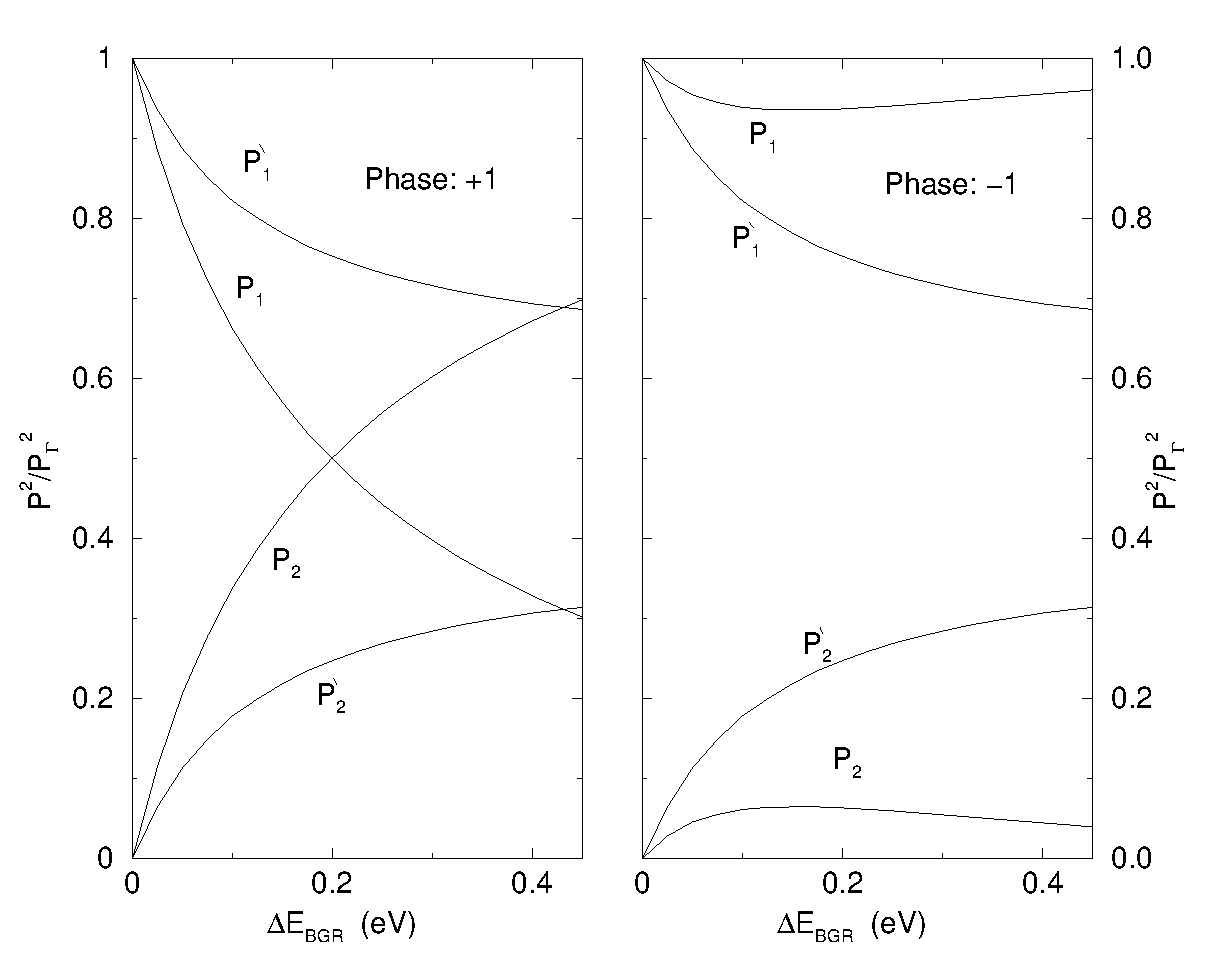
\includegraphics[width=\textwidth]{P.oV11.eps}
  \caption{Betragsquadrat der Impulsmatrixelemente aus
  Gl.~\eqref{eq:neu-k.p-H} f"ur positives und negatives relatives Vorzeichen
  von \V{11} und \V{35} in Einheiten von $|\PG|^{2}$.} 
  \label{fig:P-me.oV11}
\end{figure}


\begin{figure}[htb]
  \centering
  \includegraphics[width=\textwidth]{masses.G.oV11.eps}
  \caption{Effektive Massen von \bGCB (\GCB) f"ur positives und negatives
    relatives Vorzeichen von \V{11} und \V{35}.} 
  \label{fig:m*-GCB.oV11}
\end{figure}


\begin{figure}[htb]
  \centering
  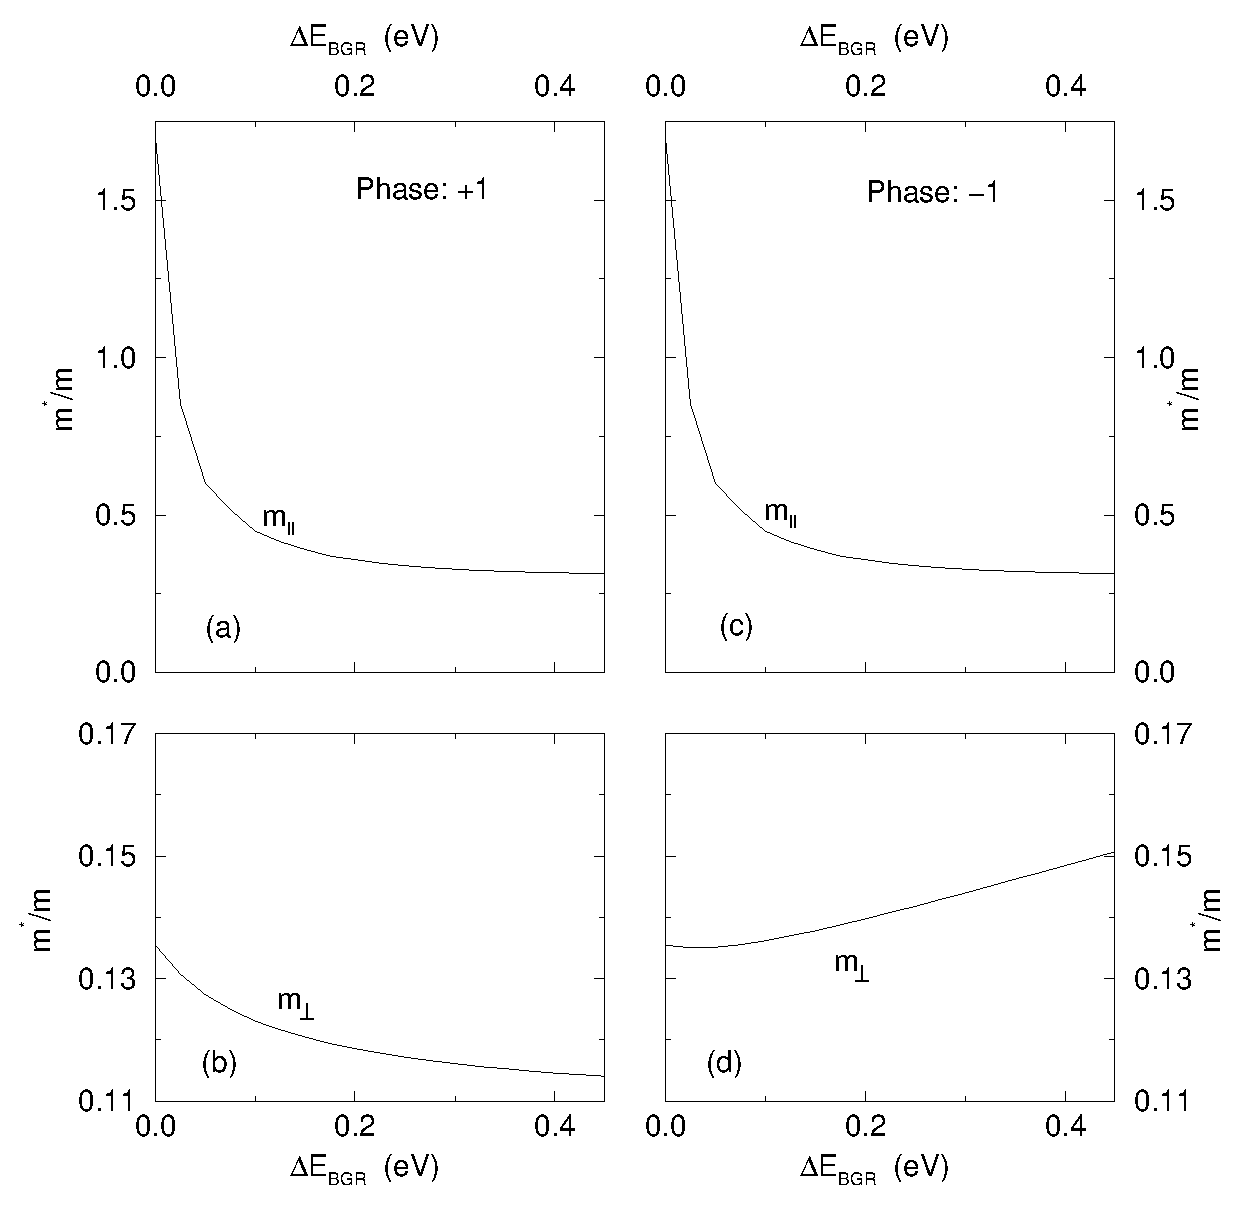
\includegraphics[width=\textwidth]{masses.L2.oV11.eps}
  \caption{Effektive Massen von \bGCB (\LCB) f"ur positives und negatives
    relatives Vorzeichen von \V{11} und \V{35}.} 
  \label{fig:m*-LCB.oV11}
\end{figure}



%%% Local Variables: 
%%% mode: latex
%%% TeX-master: "diplom"
%%% End: 

\end{appendix}

%%%%%%%%%%%%%%%%%%
\backmatter 

\addcontentsline{toc}{chapter}{Literaturverzeichnis}

%\bibliographystyle{unsrt}
%\bibliographystyle{plain}
\bibliographystyle{myprsty}
\bibliography{journal,kp,gainp,tba}

% Best?tigung und Danksagung
%%% Danksagungen
%%% Time-stamp: <1999-03-04 14:17:00 ralf>


\chapter{Danksagung}
\label{cha:danke}

Zum Gelingen dieser Arbeit haben verschiedene Personen beigetragen, bei denen
ich mich hiermit bedanken m"ochte:\\[-0.3ex]

\emph{Prof.~Dr.~O.~Pankratov} f"ur die "Uberlassung der Diplomarbeit, den
Freiraum bei ihrer Bearbeitung und die vielen wertvollen Hinweise.\\[-1.5ex]

\emph{Roland Winkler} f"ur die sehr gute Betreuung und die vielen
interessanten Diskussionen.\\[-1.5ex]

\emph{Thomas Kippenberg} und \emph{Jan Krau"s} (Institut f"ur Technische
Physik I der U Erlangen), die mir die experimentelle Seite von \GaInP\ zeigten
und immer wieder interessante Fragen hatten.\\[-1.5ex]

\emph{Dr.~R.~Scholz} (TU Chemnitz) f"ur Hinweise zur LCAO-Methode.\\[-1.5ex]

\emph{Markus Horme"s} (Institut f"ur Theoretische Physik I der U Erlangen),
der mich durch seine Fragen anregte.\\[-1.5ex]
 
Allen anderen am Lehrstuhl, f"ur Aufmunterung und viele Tips sowie
insbesondere \emph{Oliver Beckstein}, \emph{Peter Fleck} und \emph{Alexander
  Mattausch} daf"ur, da"s sie mich als "`Nicht-Numeriker"' bei ihnen im Zimmer
geduldet haben. 



%%% Local Variables: 
%%% mode: latex
%%% TeX-master: "diplom"
%%% End: 

%%% Selbstst�ndigkeitserkl�rung
%%% Time-stamp: <1999-03-04 14:16:56 ralf>


\pagestyle{empty}



\vspace*{8cm}\noindent
Hiermit versichere ich, diese Arbeit selbstst"andig und unter
ausschlie"slicher Verwendung der angegebenen Literatur angefertigt zu
haben.\\[1.5cm] 

Erlangen, den 5. M"arz 1999\\[0.7cm]

\hspace*{8cm}Ralf Stubner

%%% Local Variables: 
%%% mode: latex
%%% TeX-master: "diplom"
%%% End: 


\end{document}


%%% Local Variables: 
%%% mode: latex
%%% TeX-master: t
%%% End: 




